\documentclass[a4paper,fleqn]{report} 
%\usepackage{refcheck}

% All the packages and general definitions are included in this file: preamble.tex
\usepackage{color}
\usepackage{listings}
\usepackage[utf8]{inputenc}
\usepackage[page,toc,titletoc,title]{appendix}
% \usepackage{hyperref}
\usepackage{cite}
\usepackage{amsmath,amssymb,amsfonts}
\usepackage{algorithmic}
\usepackage{graphicx}
\usepackage{textcomp}
\usepackage{xcolor}
\usepackage{multicol}
\usepackage{physics}
\usepackage{amsthm}
%\usepackage{xepersian}
\usepackage{bm}
\newtheorem{theorem}{قضیه}
\newtheorem{definition}{تعریف}
\newtheorem{example}{مثال}
\newtheorem{lemma}{لم}
\newtheorem{case}{حالت}
\newtheorem{assumption}{فرضیه}

%\usetheme{}
\usepackage{amsthm}
\usepackage{mathtools}
%\usepackage{physics}
\usepackage{calligra}
\usepackage{csquotes}

\usepackage[thicklines]{cancel}
\usepackage{tcolorbox}
%\usepackage{pstricks}
\usepackage{wrapfig}
\usepackage[backend=biber, bibstyle=nature, sorting=nty, citestyle=numeric-comp]{biblatex} %Custom bibliography
    \addbibresource{bib.bib} %Load references

 \setbeamertemplate{navigation symbols}{} 
\DeclareMathAlphabet{\mathcalligra}{T1}{calligra}{m}{n}
\DeclareFontShape{T1}{calligra}{m}{n}{<->s*[2.2]callig15}{}
\newcommand{\scriptr}{\mathcalligra{r}\,}
\newcommand{\boldscriptr}{\pmb{\mathcalligra{r}}\,}
\def\rc{\scriptr}
\def\brc{\boldscriptr}
\def\hrc{\hat\brc}
\newcommand{\ie}{\emph{i.e.}} %id est
\newcommand{\eg}{\emph{e.g.}} %exempli gratia
\newcommand{\rtd}[1]{\ensuremath{\left\lfloor #1 \right\rfloor}}
\newcommand{\dirac}[1]{\ensuremath{\delta \left( #1 \right)}}
\newcommand{\diract}[1]{\ensuremath{\delta^3 \left( #1 \right)}}
\newcommand{\e}{\ensuremath{\epsilon_0}}
\newcommand{\m}{\ensuremath{\mu_0}}
\newcommand{\V}{\ensuremath{\mathcal{V}}}
\newcommand{\prnt}[1]{\ensuremath{\left(#1\right)}} %parentheses
\newcommand{\colch}[1]{\ensuremath{\left[#1\right]}} %square brackets
\newcommand{\chave}[1]{\ensuremath{\left\{#1\right\}}}  %curly brackets

\useoutertheme[subsection=false]{miniframes}
\setbeamertemplate{mini frame in other section}{}
%\usepackage{etoolbox}
%\makeatletter
%\let\beamer@section@set@min@width=\relax
%\patchcmd{\insertnavigation}{\hskip-1.875ex plus-1fill}{}{}{}
%\patchcmd{\sectionentry}{\hskip1.875ex plus 1fill}{}{}{}
%\patchcmd{\sectionentry}{\hyperlink{Navigation#3}{{\usebeamertemplate{section in head/foot shaded}}}}{}{}{}
%\patchcmd{\slideentry}{\usebeamertemplate{mini frame in other subsection}}{\usebeamertemplate{mini frame in other subsection of current section}}{}{}
%\patchcmd{\slideentry}{\usebeamertemplate{mini frame in other subsection}}{\usebeamertemplate{mini frame in other section}}{}{}
%\patchcmd{\slideentry}{\usebeamertemplate{mini frame in other subsection of current section}}{\usebeamertemplate{mini frame in other subsection}}{}{}
%\patchcmd{\insertnavigation}{\hskip.3cm}{\hfill}{}{}\patchcmd{\insertnavigation}{\hskip.3cm}{\hfill}{}{}
%\makeatother


%\useoutertheme{infolines}
\useinnertheme{rectangles}
\usefonttheme{professionalfonts}


% ------------------------ colors

\definecolor{orange}{HTML}{4F517D}
\definecolor{gray}{HTML}{FFFFFF}
\definecolor{yellow}{HTML}{A997DF}
\definecolor{lightorange}{HTML}{DCCFEC}

\renewcommand{\CancelColor}{\color{orange}}

% -----------------------------

\makeatletter
\newcommand{\mybox}[1]{%
  \setbox0=\hbox{#1}%
  \setlength{\@tempdima}{\dimexpr\wd0+13pt}%
  \begin{tcolorbox}[colback=orange,colframe=orange,boxrule=0.5pt,arc=4pt,
      left=6pt,right=6pt,top=6pt,bottom=6pt,boxsep=0pt,width=\@tempdima]
    \textcolor{white}{#1}
  \end{tcolorbox}
}
\makeatother

\usecolortheme[named=orange]{structure}
\usecolortheme{sidebartab}
\usecolortheme{orchid}
\usecolortheme{whale}
\setbeamercolor{alerted text}{fg=yellow}
\setbeamercolor{block title alerted}{bg=alerted text.fg!90!black}
\setbeamercolor{block title example}{bg=lightorange!60!black}
\setbeamercolor{background canvas}{bg=gray}
\setbeamercolor{normal text}{bg=gray,fg=black}

\setbeamertemplate{footline}
        {
      \leavevmode%
      \hbox{%
      \begin{beamercolorbox}[wd=.333333\paperwidth,ht=2.25ex,dp=1ex,center]{author in head/foot}%
        \usebeamerfont{author in head/foot}
      \end{beamercolorbox}%
      \begin{beamercolorbox}[wd=.333333\paperwidth,ht=2.25ex,dp=1ex,center]{title in head/foot}%
        \usebeamerfont{title in head/foot}\insertshorttitle
      \end{beamercolorbox}%
      \begin{beamercolorbox}[wd=.333333\paperwidth,ht=2.25ex,dp=1ex,center]{date in head/foot}%
        \usebeamerfont{date in head/foot}\insertshortdate{}%\hspace*{2em}

    %#turning the next line into a comment, erases the frame numbers
        \insertframenumber{} / \inserttotalframenumber\hspace*{2ex} 

      \end{beamercolorbox}}%
      \vskip0pt%
    }


\setbeamertemplate{blocks}[rectangle]
\setbeamercovered{dynamic}

\setbeamertemplate{section page}
{
	\begin{centering}
		\begin{beamercolorbox}[sep=27pt,center]{part title}
			\usebeamerfont{section title}\insertsection\par
			\usebeamerfont{subsection title}\insertsubsection\par
		\end{beamercolorbox}
	\end{centering}
}

\setbeamertemplate{subsection page}
{
	\begin{centering}
		\begin{beamercolorbox}[sep=12pt,center]{part title}
			\usebeamerfont{subsection title}\insertsubsection\par
		\end{beamercolorbox}
	\end{centering}
}

\newcommand{\hlight}[1]{\colorbox{violet!50}{#1}}
\newcommand{\hlighta}[1]{\colorbox{red!50}{#1}}

\AtBeginSection[]{
	
	\begin{frame}
		\tableofcontents[sectionstyle=show/shaded,subsectionstyle=show/shaded/hide,subsubsectionstyle=show/shaded/hide]
	\end{frame}
}

\AtBeginSubsection[]{

	\begin{frame}
		\tableofcontents[sectionstyle=show/shaded,subsectionstyle=show/shaded/hide,subsubsectionstyle=show/shaded/hide]
	\end{frame}
}	

\begin{document}

% The first pages (before abstract) are included in this file: firstpages.tex
%*************************************************
% In this file the first few pages are typeset.
% Make the changes accordingly
%*************************************************

% شماره صفحات با حروف
\pagenumbering{adadi}

%***************************
% 1st page: Blank
%***************************
\thispagestyle{empty}
\mbox{}
\pagebreak

%***************************
% 2nd page: Besmelah
%***************************
\thispagestyle{empty}
\begin{center}
	~\vfill
	\includegraphics[scale=1]{besm1.jpg}
	~\vfill
\end{center}
\pagebreak

%***************************
% 3rd page: Title
%***************************
\thispagestyle{empty}
%\pagenumbering{gobble}
\newgeometry{left=3cm,right=3cm,top=2cm}
\begin{center}
\includegraphics[height=3cm]{iut_logo.png}
\vspace{0.4cm}

\textbf{دانشگاه صنعتی اصفهان}\\
\vspace{0.4cm}

{\large

	دانشکده مهندسی برق و کامپیوتر
}
\vspace{3cm}

\Huge{\textbf{بررسی کمینه‌ها در مسائل }}\\
\vspace{0.5cm}
{\Huge
	\textbf{پيچيدگي ارتباطی كوانتومي }\\
}
\vspace{0.5cm}
\Huge{\textbf{در حوزه ساختمان داده‌ها}}
\vspace{2.5cm}

{\huge
	گزارش پروژه\\
}
\vspace{1cm}

{\Large
	\textbf{نگار سخایی}\\
}
\vspace{1.5cm}

{\Large
	 اساتید راهنما\\
}
\vspace{0.8cm}

{\Large
	\textbf{دکتر مریم موزرانی}\\

}
\vspace{0.5cm}
{\Large
	\textbf{دکتر رامین جوادی}\\

}
\vspace{1.5cm}
\large{\today}




\end{center}
\restoregeometry
\pagebreak

%%***************************
%% 5th page: Acknowledgment
%%***************************
%\thispagestyle{empty}
%\newgeometry{left=3cm,right=4cm,top=4cm}
%\vspace*{1.5cm}
%
%{\large
%	\textbf{تشکر و قدردانی}\\
%
%	
%پروردگار منّان را سپاسگزارم ......
%
%}
%\restoregeometry
%\pagebreak

%***************************
% 6th page: Rights
%***************************

%\thispagestyle{empty}
%\newgeometry{left=6cm,right=6cm}

%\begin{spacing}{3}
%\leavevmode
%\vfill
%\parbox{8 cm}{

%\textbf{\Large کلیه حقوق مادی مترتب بر نتایج مطالعات، ابتکارات و نوآوری‌های ناشی از تحقیق موضوع این پایان‌نامه  متعلق به دانشگاه صنعتی اصفهان است.}

%}
%\vfill
%\end{spacing}
%\restoregeometry
%\pagebreak

%%***************************
%% 7th page: Dedication
%%***************************
%\thispagestyle{empty}
%\vspace*{4cm}
%
%{\LARGE
%\centering
%\textbf{تقدیم به \\ پدر و مادر عزیزم }
%
%}
%\pagebreak


%***************************
%  Blank
%***************************
%\thispagestyle{empty}
%\mbox{}
%\pagebreak

%***************************
% 8th page: Table of contents
%***************************

\titleformat{\chapter}[display]
	{\normalfont\LARGE\bfseries\centering}{\chaptertitlename ~ \tartibi{chapter}}{20pt}{\LARGE}
\newgeometry{left=2.5cm,right=3cm,top=3cm,bottom=2.5cm,includehead=false,headsep=1cm,footnotesep=.5cm}
\baselineskip=.7cm

\addtocontents{toc}{\textbf{\underline{عنوان}}}
\addtocontents{toc}{\hfill\textbf{\underline{صفحه}}\par}
\addcontentsline{toc}{section}{فهرست مطالب}
\tableofcontents
\pagebreak


% change the font and margins of a chapter title
\titlespacing*{\chapter}{0pt}{3.5cm}{6cm}
\titleformat{\chapter}[display]
	{\normalfont\LARGE\bfseries\raggedright}{\chaptertitlename ~ \tartibi{chapter}}{20pt}{\LARGE}

% No page numbers on the first page of a chapter
\assignpagestyle{\chapter}{empty}
	
						
%% The abstract of the paper goes here: abstract.tex
%%*************************************************
% In this file the abstract is typeset.
% Make changes accordingly.
%*************************************************

\addcontentsline{toc}{section}{چکیده}
\newgeometry{left=2.5cm,right=3cm,top=3cm,bottom=2.5cm,includehead=false,headsep=1cm,footnotesep=.5cm}
\setcounter{page}{1}
\pagenumbering{arabic}						% شماره صفحات با عدد
\thispagestyle{empty}

~\vfill

\subsection*{چکیده}
\begin{small}
\baselineskip=0.7cm

\vspace*{0.5 cm}

\noindent\textbf{واژه‌های کلیدی:}

\end{small}								

%*****************************************************************
%% تنظیم مناسب صفحه و فونت برای متن اصلی پایان‌نامه
\newgeometry{left=2.5cm,right=3cm,top=3cm,bottom=2.5cm,includehead=false,headsep=1cm,footnotesep=.5cm}

% \setdigitfont{Times New Roman}
% \DefaultMathsDigits

\settextfont[ExternalLocation]{Zar.ttf}\fontsize{12}{6}\selectfont
\baselineskip=.9cm



% Moving page number to top right
\pagestyle{myheadings}

\bibliographystyle{acm}
%*****************************************************************

% Main chapters
\chapter{مقدمه}\label{intro}
مباحث نظری مربوط به پیچیدگی ارتباطی، پس از طرح اولیه آن‌ها توسط Yao در سال 1979، در حیطه‌های مختلفی استفاده شده‌اند. 
	این کاربرد‌ها، در زمینه‌‌های متنوعی مانند الگوریتم‌های جریانی، نظریه بازی‌ها‌‌ طراحی مدارهای VLSI و ... یافت می‌شوند.
	در نتیجه، این کاربردهای متنوع تحقیقات زیادی را در این زمینه شامل شده است.\\
	
محاسبات کوانتومی، مبحث جدیدی در علوم کامپیوتر است که با وجود عمر کوتاه، تغییرات زیادی را در تصور و درک ما نسبت به نظریه محاسبات و پیچیدگی محاسباتی ایجاد کرده است. 
طراحی و انتشار این الگوریتم‌ها - مانند الگوریتم شور \footnote{Shor} برای به‌دست آوردن عوامل اول یک عدد دلخواه در زمان بهینه - محققان را به پرسش این سوال دعوت می‌کند که آیا در مباحث و حوزه‌های دیگر پیچیدگی محاسباتی نیز، امکان یافت الگوریتم‌های بهینه‌تری وجود دارد یا خیر؟\\

در ادامه، پس از معرفی این حوزه‌ها و مباحث نظری پایه‌ای موردنیاز، به بررسی چند مسئله به شکل بالا می‌پردازیم و تلاش می‌کنیم با شبیه‌سازی آن‌ها، از پیچیدگی و زمان اجرای آن‌ها مطلع شویم.\\


مباحث نظری مربوط به پیچیدگی ارتباطی، پس از طرح اولیه آن‌ها توسط Yao در سال 1979، در حیطه‌های مختلفی استفاده شده‌اند. 
	این کاربرد‌ها، در زمینه‌‌های متنوعی مانند الگوریتم‌های جریانی، نظریه بازی‌ها‌‌ طراحی مدارهای VLSI و ... یافت می‌شوند.
	در نتیجه، این کاربردهای متنوع تحقیقات زیادی را در این زمینه حاصل کرده است.\\
	
محاسبات کوانتومی، مبحث جدیدی در علوم کامپیوتر است که با وجود عمر کوتاه، تغییرات زیادی را در تصور و درک ما نسبت به نظریه محاسبات و پیچیدگی محاسباتی ایجاد کرده است. 
طراحی و انتشار این الگوریتم‌ها - مانند الگوریتم شور \footnote{Shor} برای به‌دست آوردن عوامل اول یک عدد دلخواه در زمان بهینه - محققان را به پرسش این سوال دعوت می‌کند که آیا در مباحث و حوزه‌های دیگر پیچیدگی محاسباتی نیز، امکان یافت الگوریتم‌های بهینه‌تری وجود دارد یا خیر؟\\

در این پروژه، پس از معرفی این حوزه‌ها و مباحث پایه‌ای موردنیاز، به بررسی چند مسئله نظری به شکل بالا می‌پردازیم و در نهایت تلاش می‌کنیم با شبیه‌سازی آن‌ها، از پیچیدگی و زمان اجرای آن‌ها مطلع شویم.\\

بررسی کمینه‌ها در مسائل پيچيدگي ارتباطی كوانتومي در حوزه ساختمان داده‌ها
فصل‌های دوم تا چهارم، به مباحث تئوری بنیادین پیچیدگی ارتباطی - پیچیدگی قطعی، غیرقطعی و تصادفی - می‌پردازند. سپس در فصل پنجم، کاربرد خاصی از آن‌ها در حالت کلاسیک مطرح شده و نتایخ به مشاهده‌شده را برای به‌دست آوردن نتایجی در آن زمینه‌ها بیان خواهند شد.\\

از فصل ششم، مکانیک کوانتومی معرفی خواهد شد. این فصل مقدمه تاریخی و نظری روی اصول مکانیک کوانتومی و پدیده‌های غیرمنتظره آن‌هاست. در این فصل، دانش کلی‌ای در مورد جبرخطی و ریاضیات موردنیاز فرض شده است و به همین دلیل، در پیوست اول مقدمه‌ای بر مبانی ریاضی مکانیک کوانتومی آورده شده است.\\

در دو فصل بعد، الگوریتم‌های کوانتومی را بررسی می‌کنیم. فصل هفتم در مورد الگوریتم‌های معروف را مطرح می‌کند و فصل هشتم، حالت توزیع‌شده و ارتباطی آن‌ها را بررسی خواهد کرد.
در نهایت، فصل آخر شبیه‌سازی چندی از این الگوریتم‌ها را دربرخواهد داشت.
\chapter{پیچیدگی ارتباطی}\label{chapter1}


\par
مدل پیچیدگی ارتباطی در ابتدا در سال 1970 توسط Yao معرفی شد و هدف آن این است که یک مساله‌ را به صورت توزیع‌شده\footnote{Distributed} حل کند. منظور از حل به صورت توزیع‌شده آن است که افراد مختلف، با در دست داشتن آرگومان‌های مختلف از یک مساله مشخص، با همکاری هم به حل مساله بپردازند. مهم‌ترین نکته در این مدل این است که افراد دخیل در مخابره، قدرت محاسباتی نامحدود دارند و تنها فاکتور مورد بررسی، مقدار پیام‌های رد و بدل شده میان آ‌ن‌هاست.
 مطالب این فصل با اقتباس از 
 \cite{ 
 		nissan09,
 		lee09,
 		tim15,
 		toni14,
 		sherstov18
 		}
 تهیه شده است.


\section{تعریف}

یک پروتکل قطعی پیچیدگی ارتباطی، پروتکلی مانند $\pi$ است که در هر مرحله، یکی از دو طرف مخابره، پیامی یک بیتی به دیگری می‌فرستد. آلیس (A) ورودی $x \in X$ را در اختیار دارد و باب (B) ورودی $y \in Y$. هدف این پروتکل این خواهد بود که این دو نفر با هم خروجی $z \in Z$ را محاسبه کنند، به صورتی که:
\[val(\pi(x, y)) = f(x, y) \quad \forall x \in X, y \in Y\]
که در آن $f$ یک تابع دانسته توسط دو طرف است.
\par

\textbf{  درخت پروتکل: }
معادل با تعریف بالا، می‌توان یک درخت پروتکل باینری در نظر گرفت که رئوسش تصمیم‌ها (بیت‌های ارسال شده) توسط بازیکنان و برگ‌هایش خروجی‌ها هستند:

\begin{itemize}
    \item هر یک از رئوس غیر برگ درخت یا به آلیس تعلق دارند و یا باب.
    \item هر راس داخلی $v$ که به آلیس تعلق دارد، معادل با تابع $A_v: X \rightarrow \{0,1\}$ است که بیت فرستاده‌شده توسط آلیس را وقتی به این راس برسد، با توجه به ورودی وی تعیین می‌کند.
    \item هر راس داخلی $v$ که به باب تعلق دارد، معادل با تابع $B_v: X \rightarrow \{0,1\}$ است که بیت فرستاده‌شده توسط باب را وقتی به این راس برسد، با توجه به ورودی وی تعیین می‌کند.
    \item هر برگ این درخت ($l$) یک مقدار $val(l) \in Z$ دارد.
\end{itemize}

هر جفت ورودی $x \in X, y \in Y$ در مدل قطعی، یک مسیر یکتا از ریشه تا یک برگ را تعیین می‌کنند. هزینه یک پروتکل، معادل با عمق درخت (بلندترین مسیر از ریشه تا برگ) است که با $D(f)$ مشخص می‌شود.

\par
از آنجایی که آلیس می‌تواند کل رشته‌اش را برای باب بفرستد و این حداکثر مکالمه مورد نیاز بین دو طرف است، برای یک تابع $f: \{0,1\}^n \times \{0,1\}^n \rightarrow \{0, 1\}$، $D(f) \leq n + 1 $ است.

\par

نکته قابل توجه این است که همواره می‌توان یک درخت پروتکل را متوازن کرد. به عبارت دیگر، یک درخت پروتکل با $N$تا برگ با درخت پروتکل دیگری با عمق $O(log\ N)$ معادل است. به بیان دیگر، عمق درخت به عنوان یک شاخص برای اندازه‌گیری پیچیدگی ارتباطی، به جز یک ضریب ثابت، با لگاریتم تعداد برگ‌های درخت معادل است.


\section{تکنیک‌های کمینه‌یابی}
زمانی که صحبت از پیچیدگی به میان می‌آید، لازم است که مشخص شود یک مساله مشخص حداقل به چه مقدار زمان یا حافظه برای رسیدن به جواب نیاز دارد. در مورد مسائل پیچیدگی ارتباطی، پیچیدگی مورد نظر همان تعداد بیت مخابره شده بین افراد مکالمه است. منظور از کمینه\footnote{lower-bound} برای این نوع پیچیدگی، کمترین تعداد بیت‌هایی است که بین دو نفر جابه‌جا خواهد شد تا پاسخ مساله $p$ با سایز ورودی $n$
بر دو طرف آشکار باشد. در مورد پیچیدگی ارتباطی و کمینه‌هایش در ابتدای راه قرار داریم ولی در حال حاضر تکنیک‌های سومندی برای مشخص کردن کمینه یک مساله تعریف و استفاده شده‌اند که ابتدا مفاهیم اولیه پیش‌نیاز را مطرح خواهیم کرد و در ادامه به بررسی هر یک از ابزارها می‌پردازیم.

\subsection{ماتریس مشخصه}
با توجه به تابع از قبل مشخص $f: X \times Y \rightarrow \{0, 1\}$، ماتریس مشخصه\footnote{Characteristic Matrix} تابع $f$ به صورت زیر است:
\begin{center}

    $M_{f} = [f(x,y)]_{x \in X, y \in Y}$

\end{center}
اگر $X=\{x_{1}, x_{2},...,x_{m}\}$ و $Y=\{y_{1}, y_{2},...,y_{n}\}$، شکل ماتریس $M_{f}$ موردنظر به صورت زیر است:
\begin{center}
    $\begin{bmatrix}
         f(x_{1}, y_{1}) & f(x_{1}, y_{2}) & \cdots & f(x_{1}, y_{n}) \\[10pt]
         f(x_{2}, y_{1}) & f(x_{2}, y_{2}) & \cdots & f(x_{2}, y_{n}) \\[10pt]
         \vdots & \vdots & \ddots & \vdots \\[10pt]
         f(x_{m}, y_{1}) & f(x_{m}, y_{2}) & \cdots & f(x_{m}, y_{n})
    \end{bmatrix}$
\end{center}


توجه کنید که که در مبحث پیچیدگی ارتباطی، می‌توانیم از تمامی هزینه‌ها به جز بیت‌های مخابره شده صرف نظر کنیم، چرا که برای هر یک از شرکت کنندگان قدرت محاسباتی بی‌نهایت در نظر گرفته‌ایم.

\subsection{پروتکل، درخت و مستطیل‌ها ‌}
قبلا در مورد نمایش درختی یک پروتکل صحبت کردیم، اینجا می‌خواهیم ارتباط بین پروتکل، درخت و مستطیل را نشان می‌دهیم.
\begin{figure}[h]
    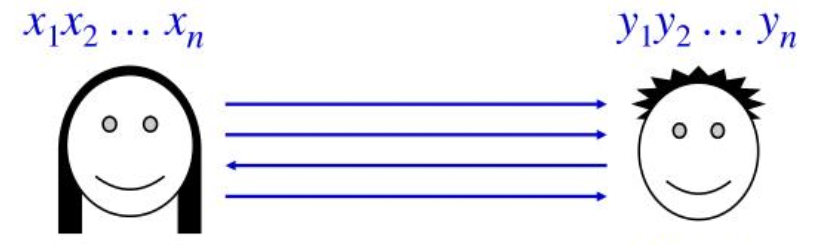
\includegraphics[width=8cm]{1}
    \centering
    \label{fig:001}
    \caption{ماتریس مشخصه یک تابع دلخواه $f: X \times Y \rightarrow \{0, 1\}$ با $X = Y = \{00, 01, 10, 11\}$.}
\end{figure}
به منظور تفهیم‌ بهتر، فرض کنید که $X = Y = \{00, 01, 10, 11\}$ و تابع $f : X \times Y \rightarrow \{0,1\}$ به واسطه ماتریس مشخصه خود در \ref{fig:001} داده شده باشد. یک پروتکل معتبر برای $f$ در شکل \ref{fig:002} نشان داده شده است.
\begin{figure}[h]
    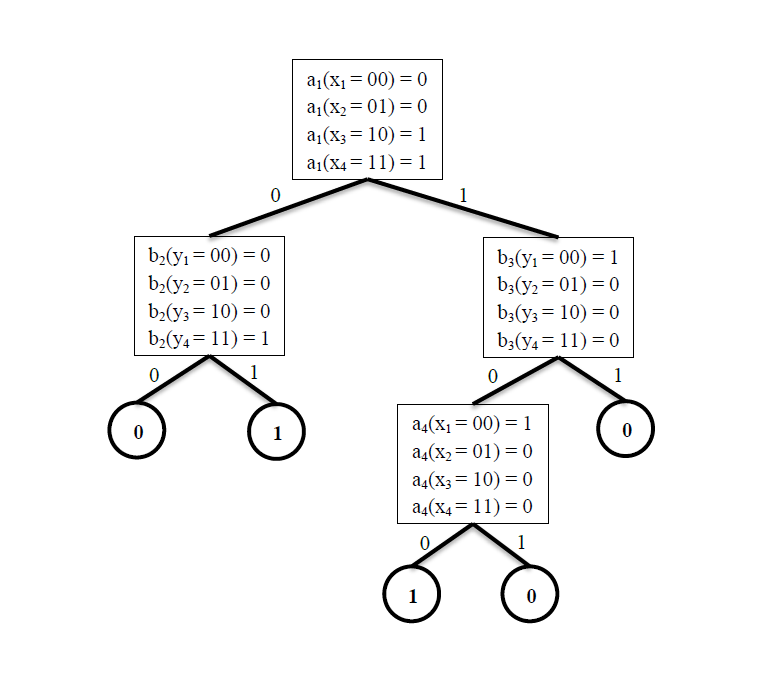
\includegraphics[width=13cm]{2}
    \centering
    \label{fig:002}
    \caption{یک پروتکل صحیح برای مخابره تابع مشخص‌شده در \autoref{fig:001}}
\end{figure}

\subsection{قطعه بندی}
\par
\begin{definition}
تابع  $f : X \times Y \rightarrow \{0,1\} $ را در نظر بگیرید. یک زیر مجموعه $ S \subseteq X \times Y$ $f$- تک‌رنگی\footnote{f-monochromatic} است اگر تابع $f$ روی $S$ ثابت باشد.
\end{definition}

\begin{theorem}
مجموعه ورودی‌های $(x,y) \in X \times Y$ که به یک برگ مشخص از درخت پروتکل ختم می‌شود، یک مستطیل است.
\end{theorem}

نتیجه: هر پروتکل قطعی برای تابع $f$، مجموعه  $X \times Y $ را به مستطیل‌های $f$-تک‌رنگی جدا از هم قطعه‌بندی\footnote{partition} می‌کند. در واقع، حداکثر تعداد مستطیل‌ها $2^{C}$ است که $C$ هزینه ارتباطی پروتکل است (ارتفاع درخت).
\\
بیشینه‌ای که در نتیجه فوق مطرح شده‌است از جایی بر‌می‌آید که درختی با ارتفاع $C$ نمی‌تواند بیشتر از $2^{C}$ برگ داشته باشد.\\
توجه کنید که هر پروتکل، ماتریس مشخصه را به تعدادی مستطیل قطع بندی خواهد کرد ولی هر قطعه‌بندی لزوما معادل یک پروتکل نیست. به عنوان مثال، در شکل \ref{fig:003} نمی‌توان یک پروتکل پیدا کرد چرا که هیچ برشی نیست که بتواند یک زیرماتریس را به دو ماتریس‌ دیگر تبدیل کند  (اولین قدم پروتکل اجرایی نیست).
\begin{figure}[h]
    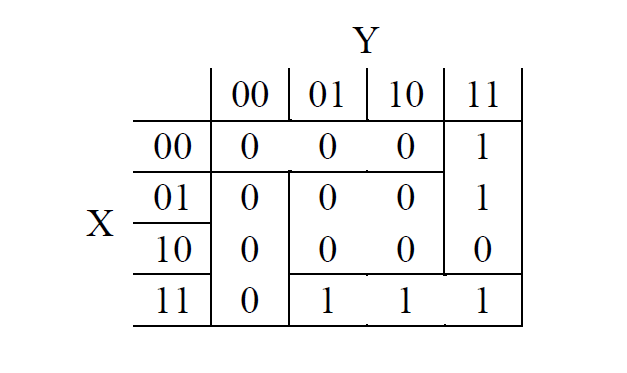
\includegraphics[width=13cm]{3}
    \centering
    \label{fig:003}
    \caption{قطع‌بندی‌ای که نمی‌تواند به یک پروتکل نظیر شود. هیچ برشی در قطعه‌بندی وجود ندارد که با انتخاب آن، ماتریس به دو زیرماتریس تبدیل شود.}
\end{figure}

\subsection{مجموعه گول‌زننده}
به عنوان یک روش برای محاسبه کردن کمینه پیچیدگی ارتباطی یک مساله، می‌توانیم از ابزاری به نام مجموعه گول زننده\footnote{Fooling Set} استفاده کنیم.\\
\begin{definition}
تابع $f : X \times Y \rightarrow \{0,1\}$ داده شده است. یک مجموعه $S \subseteq X \times Y$ را مجموعه گول زننده می‌نامند اگر یک مقدار $z \in \{0,1\}$ وجود داشته باشد به طوری که:
\begin{itemize}
    \item برای هر $(x,y) \in S$ داشته باشیم $f(x,y) = z$.
    \item برای هر دو عضو متفاوت $(x_{1},y_{1})$ و $(x_{2},y_{2})$ در $S$، یا $f(x_{1}, y_{2}) \neq z$ یا $f(x_{2}, y_{1}) \neq z$.
\end{itemize}
\end{definition}
\begin{theorem}
 پیچیدگی ارتباطی تابع $f$ از نامساوی زیر پیروی می‌کند، \\
$D(f) \geq log_{2}|S|$\\
که $S$ هر مجموعه گول زننده‌ای برای $f$ است.
\end{theorem}
\begin{proof}
هیچ دوعضوی از مجموعه گول‌زننده $S$ طبق تعریف نمی‌توانند عضو یک مستطیل در قطعه‌بندی باشند، درنتیجه حداقل به تعداد اعضای $S$، مستطیل $f$-تک‌رنگی داریم. طبق نتیجه قبل، حکم ثابت می‌شود.

\end{proof}
\begin{example}
تابع مساوی را در نظر بگیرید. از قبل می‌دانیم حداکثر تعداد بیت‌هایی که باید برای این مساله مخابره شود $n$ است. حال می‌خواهیم نشان دهیم که این تعداد، حداقل هم هست. تعریف تابع مساوی$EQ_{n} : \{0,1\}^{n} \times \{0,1\}^{n} \rightarrow \{0,1\}$ به صورت زیر خواهد بود
\begin{equation}
    EQ_{n}(x,y) =
    \begin{cases}
        1 & \text{ x=y}\\
        0 & \text{در غیر این صورت}
    \end{cases}
\end{equation}

ماتریس مشخصه این تابع همان ماتریس همانی $2^{n} \times 2^{n}$ است.
\begin{center}
    $\begin{bmatrix}
         1 & 0 & \cdots & 0 \\
         0 & 1 & \cdots & 0 \\
         \vdots & \vdots & \ddots & \vdots \\
         0 & 0 & \cdots & 1
    \end{bmatrix}$
\end{center}
مجموعه گول زننده در این حالت همه مقادیر $1$ تابع $f$ است. چرا که هیچ دوتایی از ورودی‌هایی که خروجی $1$ دارند، در یک مسنطیل نمی‌توانند باشند.  \\
\end{example}
\subsection{کران اندازه مستطیل}
کران اندازه مستطیل\footnote{Rectangle Size Bounds} یک روش دیگر برای اثبات کردن کمینه‌های توابع بولی مورد استفاده در پیچیدگی ارتباطی است. ایده پشت این ماجرا، ثابت کردن آن است که اندازه هر مستطیل کوچک است، در نتیجه باید تعداد زیادی مستطیل برای پوشاندن کل ماتریس مشخصه داشته باشیم. \\
ایده: 
تابع $f : X \times Y \rightarrow \{0,1\}$ داده شده است. روی اعضای $f^{-1}(1)$ یک توزیع احتمال $\mu$ تعریف می‌کنیم به طوری که برای هر مستطیل $R$ شامل مقادیر $1$، $\mu(R) $کوچک باشد. به همین طریق می‌توانیم برای مقادیر $0$ هم این روند را تکرار کنیم. \\
\begin{example}
نشان می‌دهیم که مجموعه گول‌زننده یک مدلی از کران اندازه مستطیل است. فرض کنید که مجموعه گول‌زننده $S$ را داشته باشیم و $|S| = t$. حال $\mu$ را یک توزیع یکنواخت روی اعضای $S$ درنظر بگیرید. در نتیجه
\begin{equation}
    \mu(x,y) =
    \begin{cases}
        $1/t$ & \text{$(x,y) \in S$}\\
        0 & \text{در غیر این صورت}
    \end{cases}
\end{equation}

نشان دادیم که هیچ دو عضوی از مجموعه $S$ نمی‌توانند در یک مستطیل $f$-تک‌رنگی باشند. در نتیجه، برای هر مستطیل $R$ داریم  $\mu(R) \leq 1/t$ و در نهایت باید $\frac{1}{\frac{1}{t}}$ برگ در درخت پروتکل وجود داشته باشد و این گواهی بر این است که  $D(f) \geq \lceil \log_{2} t \rceil$.
\end{example}
\subsection{کمینه رتبه ماتریس \footnote{Matrix Rank}} % TODO : example
\begin{theorem}
تابع $f : X \times Y \rightarrow \{0,1\}$ داده شده است. داریم $D(f) \geq \log_{2}(2\times rank_{F}(M_{f} -1) )$ بر روی هر میدان $F$.
\end{theorem}
\begin{proof}
در قسمت‌های قبل نشان دادیم که پیچیدگی ارتباطی تابع مساوی برابر $n$ است. حال با استفاده از رتبه، این را نشان می‌دهیم: \\
از آنجایی که ماتریس مشخصه تابع مساوی ماتریس همانی $2^{n} \times 2^{n} $ است، و رتبه این ماتریس برابر $2^{n} $ است، طبق قضیه قبل پیچیدگی ارتباطی این مساله $n$ است.
\end{proof}



\chapter{پیچیدگی ارتباطی غیرقطعی}\label{chapter2}

در این بخش، سعی بر این است که مشابه تئوری پیچیدگی محاسباتی، مدل غیرقطعی\footnote{Non-deterministic} را در پیچیدگی ارتباطی نیز تعریف کنیم.  مطالب این فصل با اقتباس از 
 \cite{ 
 		nissan09,
 		lee09,
 		tim15,
 		toni14,
 		sherstov18,
 		laszlo86
 		}
 تهیه شده است.

برای هر تابع بولی $f: X \times Y \rightarrow \{0, 1\}$، یک پروتکل غیرقطعی دو بخش خواهد داشت. در ابتدا، یک پیشگو\footnote{Oracle} که به ورودی هر دو طرف دسترسی دارد یک رشته $a$ را به هر دو طرف می‌دهد. در مرحله دوم، بازیکنان با در اختیار داشتن این رشته و ورودی‌های خودشان، پروتکل را مانند قسمت قطعی ادامه می‌دهند و در مورد مقدار تابع تصمیم می‌گیرند. اگر خروجی را با $\Pi(x, y, a)$ نشان دهیم،  این پروتکل مقدار $f$ را به درستی محاسبه می‌کند اگر:
\[f(x, y) = 1\ \Rightarrow \exists a, \Pi(x, y, a) = 1\]
\[f(x, y) = 0\ \Rightarrow \forall a, \Pi(x, y, a) = 0\]
هزینه این پروتکل، جمع حداکثر طول رشته $a$ و حداکثر تعداد بیت‌های مخابره شده بین دو طرف است. هزینه غیرقطعی محاسبه $f$ که با $N^1(f)$ نشان داده می‌شود، حداقل هزینه پروتکلی‌ست که $f$ را محاسبه می‌کند. متناظر با این تعریف، هزینه co-nondeterministic برای تابع $f$ به همین شکل بیان و با $N^0(f)$ نشان داده می‌شود.
   
\begin{example}
تابع نامساوی را درنظر بگیرید. تعریف رسمی این تابع به شکل زیر می‌باشد:
\begin{equation}
    NEQ_{n}(x,y) =
    \begin{cases}
        0 & \text{ x=y}\\
        1 & \text{در غیر این صورت}
    \end{cases}
\end{equation}
و ماتریس مشخصه آن نیز به این شکل است:
\begin{center}
    $\begin{bmatrix}
         0 & 1 & \cdots & 1 \\
         1 & 0 & \cdots & 1 \\
         \vdots & \vdots & \ddots & \vdots \\
         1 & 1 & \cdots & 0
    \end{bmatrix}$
\end{center}
هزینه محاسبه غیرقطعی این تابع ($(N^1(NEQ$) برابر $O(\log n)$ است. برای مشاهده این موضوع، دقت کنید که اگر دو ورودی متفاوت باشند، پیشگو می‌تواند شماره بیت اختلاف را به عنوان رشته اولیه به هر دو طرف ارسال کند. در نتیجه، هزینه کل پروتکل برابر طول رشته کمک اولیه ($O(\log n)$) و هزینه چک کردن آن بیت خواهد بود. (آلیس بیت مشخص شده را برای باب ارسال می‌کند، باب مشاهده می‌کند که رشته‌ها متفاوت هستند. این عمل به یک بیت مخابره نیاز دارد.)\\
در جهت دیگر، مشاهده کنید که اگر دو ورودی با هم مساوی باشند، هیچ رشته اولیه‌ای وجود ندارد که پیشگو بتواند در ابتدا به هر دو طرف ارسال کند و فرآیند چک کردن تساوی را آسان‌تر نماید. پس برای این تابع، 
$N^0(NEQ) = O(n)$
خواهد بود.
\end{example}
\section{پوشش‌ها}

مشابه ارتباط پیچیدگی قطعی با مستطیل‌ها، پیچیدگی غیرقطعی ارتباط مستقیمی با پوشش‌ها\footnote{Covers} دارد.

\begin{definition}
برای هر $z \in \{0, 1\}$، یک $z$-پوشش\footnote{z-Cover} برای $f$، مجموعه‌ای از مستطیل‌های $R_1, \dots, R_N$ است که ممکن است اشتراک داشته باشند، به طوری که 
$f^{-1}(z) = \cup R_i$.
حداقل سایز یک z-پوشش برای $f$ را با $C^z(f) = N$ نشان .می‌دهیم
\end{definition}
\begin{theorem}
برای $z \in \{0, 1\}$ داریم: $N^z(f) = \log C^z(f) + O(1)$ به عبارت دیگر، ارتباط هزینه مخابره غیرقطعی با پوشش‌ها معادل مخابره قطعی با  مستطیل‌هاست.
\end{theorem}

\section{کلاس‌های پیچیدگی}

یکی از بزرگ‌ترین مسائل باز موجود در پیچیدگی محاسباتی، درستی تساوی $\mathbf{P} = \mathbf{NP} \cap \mathbf{coNP}$ است. در این قسمت، سعی می‌کنیم تعاریف مشابهی برای کلاس‌های متناظر آن‌ها بیان کنیم و این تساوی را در پیچیدگی ارتباطی اثبات کنیم.
\begin{definition}
 برای یک تابع دودویی $f: \{0, 1\}^n \times \{0, 1\}^n \rightarrow \{0, 1\}$ داریم:

\begin{itemize}
    \item $D(f) = polylog(n) \ \Rightarrow\ f \in \mathbf{P}^{CC}  $
     \item $N^1(f) = polylog(n) \ \Rightarrow\ f \in \mathbf{NP}^{CC}  $
     \item $N^0(f) = polylog(n) \ \Rightarrow\ f \in \mathbf{coNP}^{CC}  $
\end{itemize}

که در آن $polylog(n) = O(\log^c n)$ است.
\end{definition}
\begin{lemma} \label{lem:1}
 برای هر تابع دودویی، $D(f) = O(N^0(f)N^1(f))$
\end{lemma}
\begin{theorem}
\begin{equation*}
P^{CC} = NP^{CC} \cap coNP^{CC}
\end{equation*}
\end{theorem}
\begin{proof}
مشاهده جهت اول، مشخص است. مجموعه 
$P^{CC}$
زیر مجموعه هر دو مجموعه
$NP^{CC}$ و $coNP^{CC}$
است و پس زیرمجموعه اشتراک آن‌ها نیز خواهد بود. \\
برای اثبات قسمت دوم، مشاهده می‌کنیم که از آن‌جایی که طبق تعریف، اگر تابعی هم در 
$NP^{CC}$ و هم در $coNP^{CC}$
باشد، پس 
$N^1(f) = O(\log^{c_1} n)$ و 
$N^0(f) = O(\log^{c_2} n)$
خواهد بود. حال از لم \autoref{lem:1} استفاده می‌کنیم. 
\[D(f) = O(N^0(f)N^1(f)) \Rightarrow D(f) = O(N^0(f)N^1(f)) = O(\log^{c_1} n \  \log^{c_1} n) = O(\log^c n)\]
\end{proof}
\section{تکنیک‌های کمینه‌یابی}

تکنیک‌های کمینه‌یابی برای پیچیدگی غیرقطعی به طور مستقیم از لم قبل نتیجه می‌شوند.
\[N^1(f) \geq \Omega(\frac{D(f)}{N^0(f)})\]
و یا از معادل آن استفاده می‌کنند:\\
\begin{lemma}
 برای هر تابع دودویی، نتایج زیر برقرار است:
 \[D(f) = O(N^1(f)\.\log (\mathrm{rank}(M_f))) \Rightarrow N^1(f) \geq \Omega(\frac{D(f)}{\log (\mathrm{rank}(M_f))})\]
 \[D(f) = O(N^0(f)\.\log (\mathrm{rank}(M_f))) \Rightarrow N^0(f) \geq \Omega(\frac{D(f)}{\log (\mathrm{rank}(M_f))})\]
\end{lemma}
\section{نتیجه‌گیری}

تا به حال، چندی از ملاک‌های سنجش پیچیدگی ارتباطی را بررسی کردیم. ارتباط کلی آن‌ها به شکل زیر است:
\begin{equation}
2^{\Theta(\sqrt{D(f)})} \leq C(f) \leq C^D(f) \leq C^P(f) \leq 2^{\Theta(D(f))}
\end{equation}
\begin{itemize}
    \item $C^P(f)$ کم‌ترین تعداد برگ‌های درخت پروتکل برای تابع $f$ است.
    \item $C^D(f)$ کم‌ترین تعداد مستطیل‌ها در یک تقسیم‌بندی برای تابع $f$ است.
    \item $C^z(f)$ حداقل سایز یک z-پوشش برای تابع f است.
    \item $C(f) = C^0(f) + C^1(f)$
\end{itemize}

نامساوی اول مستقیما از لم 1 نتیجه می‌شود. دو نامساوی اول نیز در فصل قبل اثبات شده‌اند.

\chapter{پیچیدگی ارتباطی تصادفی}\label{chapter_rand}

استفاده از تصادف در بسیاری از حوزه‌های الگوریتمی، کاربرد زیادی دارد و پیچیدگی ارتباطی نیز از این امر مستثنا نیست. در این قسمت، سه مدل پیچیدگی تصادفی را بررسی خواهیم کرد و علاوه بر ارتباط آن‌ها، چند تکنیک به‌دست آوردن کمینه را نیز در نظر خواهیم گرفت. 
 \cite{nissan09,
 		lee09,
 		tim15,
 		toni14,
 		sherstov18}
 

\section{مدل سکه خصوصی}
این مدل بر فرض این که هر یک از بازیکنان به مقدار نامحدودی از بیت‌های رندوم دسترسی دارند. این مدل نیز مانند مدل قطعی، با یک درخت پروتکل قابل نمایش است.\\
تعریف درخت پروتکل برای مدل سکه خصوصی\footnote{Private Coin} به شکل زیر خواهد بود. در هر راس درخت ($v$)، توابع مشخص‌کننده مسیر $A_v , B_v$ توابع تصادفی هستند. به بیان دیگر، $A_v : X \rightarrow [0,1] $ احتمال انتخاب فرزند سمت راست را مشخص می‌کند. برای تعریف دقیق محاسبه یک تابع $f$، بیت‌های رندوم آلیس و باب را به ترتیب با $r_A, r_B$ نمایش می‌دهیم. \\
\begin{definition}
می‌گوییم پروتکل تصادفی $\Pi$ تابع $f : X \times Y \rightarrow Z$ را با خطای $\epsilon$ محاسبه می‌کند اگر:
\begin{equation}
\Pr_{r_A, r_B} [\Pi(x, y; r_A, r_B) = f(x,y)] \geq 1 - \epsilon \quad \forall x \in X, y \in Y.
\end{equation}
\end{definition}
هزینه پروتکل تصادفی مثل حالت قطعی، برابر تعداد بیت‌های مبادله‌شده (عمق درخت پروتکل) خواهد بود. حداقل هزینه پروتکلی که $ّf$ را با خطای $\epsilon$ محاسبه می‌کند را با $R_\epsilon(f)$ نمایش می‌دهیم. به علاوه، در مسائل مربوط به پیچیدگی محاسباتی $\epsilon = \frac{1}{3}$ در نظر گرفته می‌شود و داریم $R(f) = R_{\frac{1}{3}}(f)$.\\
در تمام پروتکل‌های تصادفی، می‌توان با تکرار پروتکل و انتخاب پر تکرارترین پاسخ، احتمال جواب درست را افزایش داد. در نتیجه:
\begin{equation}
R_{\epsilon}(f) = O(\log \frac{1}{\epsilon}) . R(f)
\end{equation}

\section{مدل سکه عمومی}
این مدل، فرض می‌کند بیت‌های عمومی نامحدود در اختیار آلیس و باب، مشترک هستند. این بیت‌های مشترک را با $r$ نمایش‌داده و داریم:
\begin{definition}
می‌گوییم پروتکل تصادفی $\Pi$ تابع $f : X \times Y \rightarrow Z$ را با خطای $\epsilon$ و سکه‌های عمومی\footnote{Public Coin} محاسبه می‌کند اگر:
\begin{equation}
\Pr_{r} [\Pi(x, y; r) = f(x,y)] \geq 1 - \epsilon \quad \forall x \in X, y \in Y.
\end{equation}
\end{definition}
هزینه حداقل پروتکلی که تابع $f$ را با سکه عمومی محاسبه می‌کند را با $R_\epsilon^{pub} (f)$ نمایش می‌دهیم. به شکل مشابه، از تکرار برای افزایش دقت این مدل نیز می‌توان استفاده کرد.
\begin{example}
حال از مدل‌های بررسی‌شده، برای طراحی پروتکل‌هایی برای تابع تساوی استفاده می‌کنیم. 
\begin{itemize}
\item مدل سکه خصوصی: 
\begin{enumerate}
\item آلیس یک عدد اول به صورت تصادفی از مجموعه $\{2, \dots, 2n\}$ انتخاب می‌کند.
\item آلیس عدد اول انتخاب شده ($p$) و مقدار $x \mod p$ را به باب ارسال می‌کند.
\item باب چک می‌کند که آیا $y \mod p$ برابر با عدد دریافتی هست یا خیر. اگر برابر بود 1 و اگر برابر نبود صفر برمی‌گرداند.
\end{enumerate}
مشخص است که اگر دو عدد با هم برابر باشند، نتیجه این پروتکل همواره درست خواهد بود. ولی اگر $x \neq y$ باشد، ممکن است اعداد اولی وجود داشته باشند به صورتی که $x \mod p = y \mod p$. پس در این حالت، خطا وجود خواهد داشت. حال تلاش می‌کنیم مقدار خطا را محاسبه کنیم.\\
فرض کنید که مجموعه $\{p_1, p_2, \dots, p_k\}$ مجموعه تمام اعداد اولی باشد که $x \mod p_i = y \mod p_i$. در نتیجه:
\begin{equation*}
x \mod P = y \mod P \quad P = p_1p_2\dots p_k
\end{equation*}
حال از آنجایی که $p_i \geq 2$ است، $P \geq 2^k$ خواهد بود. ولی $P$ نمی‌تواند بیش‌تر از $2^n$ باشد، چون $x \neq y$ است. پس $2^k \leq 2^n$ است و $k \leq n$ خواهد بود. حال از آنجایی که عدد اول از مجموعه‌ای به اندازه $2n$ انتخاب شده است، احتمال این که یکی از این اعداد اول به تصادف انتخاب شود کمتر از $\frac{1}{2}$ خواهد بود. (و این احتمال با تکرار می‌تواند کمتر شود.)\\
هزینه این پروتکل $O(\log n)$ است. توجه کنید که حداقل مقدار مخابره برای حالت قطعی، $O(n)$ است.
\item مدل سکه عمومی: ($r = r_1\dots r_m$ بیت‌های تصادفی مشترک‌ هستند.)
\begin{enumerate}
\item آلیس مقدار زیر را محاسبه کرده و برای باب را ارسال می‌کند:
\[\sum^n_{i=1} x_ir_i\ \mod 2\]
\item باب مقدار زیر را محاسبه کرده، با مقدار فرستاده شده توسط آلیس مقایسه می‌کند. اگر برابر بودند 1 و در غیر این صورت صفر خروجی می‌دهد.
\[\sum^n_{i=1} y_ir_i\ \mod 2\]
\end{enumerate}
همچنان مشخص است که اگر این دو ورودی با هم برابر باشند، جواب حتما درست است. ولی اگر تساوی برقرار نباشد، به احتمال $1/2$ ممکن است جواب اشتباه تشخیص داده شود و مثل حالت قبل، می‌توان با تکرار احتمال خطا را کم کرد. نکته دیگر، این است که در این مدل، فقط با فرستادن یک بیت اطلاعات نتیجه مشخص می‌شود و پیچیدگی برابر با $O(1)$ خواهد بود.
\end{itemize}
\end{example}
همان‌طور که از مثال بالا مشخص است، مدل سکه عمومی از سکه خصوصی قوی‌تر است، یعنی با مدل عمومی می‌توان بدون هزینه اضافی مدل خصوصی را شبیه‌سازی کرد، ولی نه برعکس. در نتیجه:
\[R_\epsilon^{pub} (f) \leq R_\epsilon (f)\] 
شبیه‌سازی مدل عمومی با مدل خصوصی نیز ممکن است، ولی با مقداری هزینه همراه خواهد بود. لم نیومن\footnote{Newman's lemma} نتیجه این شبیه‌سازی را بیان می‌کند.
\begin{theorem}
اگر $f : \{0,1\}^n \times \{0,1\}^n \rightarrow Z$ باشد، برای هر مقدار $\epsilon,  \delta \geq 0$ داریم:
\begin{equation}
‌R_{\epsilon+\delta}(f) \leq R_\epsilon^{pub} (f) + O(\log n + \log \frac{1}{\delta}
)
\end{equation}
\end{theorem}
\section{مدل توزیعی}\label{dist_rand}
تا به حال در تمام مدل‌های بررسی شده، عنصر تصادف در عملکرد پروتکل بوده است. در مدل توزیعی\footnote{Distributional} ورودی را تصادفی فرض می‌کنند. 
\begin{definition}
فرض کنید $\mu$ یک توزیع روی $X \times Y$ است. 
می‌گوییم پروتکل تصادفی توزیعی $\Pi$ تابع $f : X \times Y \rightarrow Z$ را با خطای $\epsilon$ و تحت $\mu$ محاسبه می‌کند اگر:
\begin{equation}
\Pr_{(x, y) \thicksim \mu} [\Pi(x, y) = f(x,y)] \geq 1 - \epsilon \quad \forall x \in X, y \in Y.
\end{equation}
\end{definition}

تکنیک‌های کمینه مدل‌های تصادفی که در بخش بعد بررسی خواهند شد، یک توزیع «دشوار» روی ورودی‌ها پیدا می‌کنند و نشان می‌دهند که هیچ پروتکل قطعی‌ و بهینه‌ای نمی‌تواند تابع مورد نظر را تحت این توزیع محاسبه کند. این تکنیک بر قضیه زیر که توسط Yao اثبات شده است مبتنی‌ست:
\begin{theorem}
اگر $f : X \times Y \rightarrow Z$ و $\epsilon \geq 0$ باشد، داریم:
\begin{equation}
\max_\mu D^\mu_{\epsilon} = R_\epsilon^{pub}(f)
\end{equation}
\end{theorem}
\section{کمینه‌یابی}
\subsection{ناهمگنی}
همانطور که در قسمت قبل بیان شد، استفاده از یک توزیع سخت، و نشان دادن کمینه‌ای برای پروتکل قطعی‌ای که ورودی را تحت آن توزیع محاسبه می‌کند، با کمینه محاسبه همان تابع توسط یک پروتکل تصادفی سکه عمومی برابر است. برای استفاده از این نکته، مفهوم جدیدی را تعریف می‌کنیم:
\begin{definition}
اگر  $f : X \times Y \rightarrow Z$ و $\mu$ یک توزیع روی $X \times Y$ باشد، می‌توان برای هر مستطیل R ناهمگنی
\footnote{Discrepancy}
را به صورت زیر تعریف کرد:
\begin{equation}
disc_\mu (f,R) = |\mu (R \cap f^{-1}(0) - \mu (R \cap f^{-1}(1)|
\end{equation}
و
\begin{equation}
disc_\mu (f) = \max_R \ disc_\mu (f,R).
\end{equation}
\end{definition}
به صورت غیررسمی، معیار ناهمنگی پایین یعنی مستطیل‌های بزرگ تعداد تقریبا برابری صفر و یک دارند. \\
این معیار را به یک شکل مشابه نیز می‌توان تعریف کرد.
در نظر بگیرید که S یک ماتریس $|X| \times |Y|$ است و هر درایه آن به شکل زیر محاسبه می‌شود:
\begin{equation*}
S_{x, y} = \mu(x,y)(-1)^{f(x,y)}.
\end{equation*}
و برای محاسبه معیار ناهمنگی:
\begin{equation}
disc_\mu (f,R) = \Bigg|\sum_{(x,y) \in R} S_{x,y}\ \Bigg|
\end{equation}

\subsection{محدودکردن مقیاس ناهمگنی و کمینه‌یابی}
\begin{theorem}
اگر برای یک تابع باینری $f$، توزیع $\mu$ وجود داشته باشد به صورتی که $disc_\mu (f) \leq 2^{-c}$ باشد، $R^{pub}_\epsilon = \Omega(c)$ خواهد بود.
\end{theorem}
با توجه به قضیه بالا، نیاز است که تکنیکی برای محدود کردن مقدار ناهمنگی بیابیم و از آن برای به‌دست آوردن کمینه‌هایی روی پیچیدگی تصادفی عمومی به‌دست آوریم. معروف ترین این تکنیک‌ها‌، تکنیک مقدار ویژه\footnote{eigenvalue} است.

\begin{lemma}
برای هر ماتریس متقارن $M$، ناهمگنی مستطیل $A \times B$ حداکثر برابر با $\lambda_{max} (M) \sqrt{|R|}$ است، که در آن $\lambda_{max}$ بزرگ‌ترین مقدار ویژه تابع است. به بیان دیگر:
\begin{equation}
disc_\mu(f, R) \leq \lambda_{max} (M) \sqrt{|A||B|}
\end{equation}
\end{lemma}
و از این تکنیک می‌توان برای به‌‌دست آوردن مقدار ناهمگنی برای بعضی از مسائل که ماتریس متقارن دارند استفاده کرد.
\chapter{کاربرد پیچیدگی ارتباطی در پردازش موازی }\label{chapter3}

در این بخش به بررسی محل تقاطع دو علم پردازش موازی و پیچیدگی ارتباطی می‌پردازیم. برای آن که متوجه باشیم چرا پژوهشگران فعال در حوزه پردازش موازی به پیچیدگی ارتباطی اهمیت می‌دهند، لازم است مقداری در مورد پردازش موازی اطلاعات کسب کنیم. در دنیای پردازش موازی، محاسبات داخلی رایگان و محاسبات بین افراد گران است. سه پیچیدگی اصلی در دنیای پردازش موازی شامل تعداد پیغام‌های رد و بدل شده (پیچیدگی پیامی \footnote{Message Complexity})، تعداد بیت‌های ردوبدل شده (پیچیدگی بیتی \footnote{Bit Complexity}) و تعداد دورهای مخابره برای یک مساله و تعدادی کاربر در یک محیط همگام (پیچیدگی دوری\footnote{Round Complexity}) می‌باشد. نکته قابل توجه برای این دو دانش از جایی برمی‌آید که پیچیدگی ارتباطی از دل پردازش موازی استخراج شده‌است و همچنین در بسیاری از مسائل با هم دیگر برابر هستند. لازم است در ادامه انواع مدل‌های پیچیدگی ارتباطی $k$-نفره را بررسی کنیم. 
\section{مدلهای پیچیدگی ارتباطی $k$نفره}

\subsection{مدل تخته‌سیاه}

در این مدل، بازیکنان با یکدیگر از طریق یک تخته سیاه ارتباط برقرار می‌کنند. هر بازیکن در نوبت خودش حق نوشتن روی تخته سیاه را دارد و پروتکل تصمیم می‌گیرد که نوبت چه کسی است. همه بازیکنان می‌توانند تخته را مشاهده کنند. در این مدل و در هنگام شبیه‌سازی، هر بیتی که نوشته می‌شود به $k-1$ بازیکن دیگر مخابره می‌شود. 

\subsection{مدل نفر-به-نفر}
یک گراف ارتباطی\footnote{Communication Graph} مشخص می‌کند که هر بازیکن به چه کسی متصل است و بدون واسطه می‌تواند پیام مخابره کند. برای راحتی کار، گراف‌های ارتباطی را گراف‌های کامل در نظر می‌گیرند که در آن هر دو بازیکن با هم ارتباط دارند. 
\begin{itemize}
	\item [همگام:] در این مدل، مخابرات در دورهای مجزا انجام می‌شو‌د. در هر دور، هر بازیکن یک پیغام می‌فرستد و پیغام‌های ورودی را دریافت می‌کند. 
	\item [ناهمگام:] در این مدل، هیچ دور مخابره‌ای وجود ندارد و هر پیغام در مواقع نیاز فرستاده می‌شود. در این مدل هر بازیکن یک صف دارد که پیغام‌ها‌ی ورودی در آن قرار می‌گیرد.
\end{itemize}
\begin{figure}[h]
	\caption{مثالی از یک مدل نفر-به-نفر 4تایی}
	\centering
	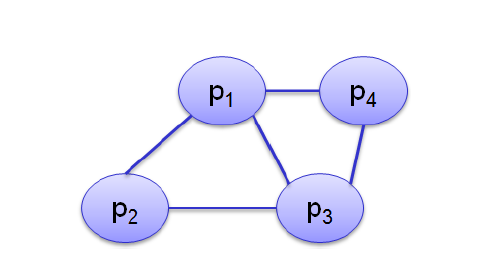
\includegraphics[width=10cm]{3_1.png}
\end{figure}
\subsection{مدل هماهنگ‌کننده}
 در این مدل، که یک حالت خاص از مدل نفر-به-نفر است، تمامی $k$ بازیکن به یک نفر و فقط یک نفر دیگر متصل هستند (در مجموع $k+1$ بازیکن) و بازیکنان از طریق این یک هماهنگ‌کننده با هم در ارتباط هستند. 
 \begin{itemize}
 	\item [همگام:] در هر دور، هر بازیکن یک پیغام به هماهنگ‌کننده می‌فرستد و هماهنگ‌کننده به آنها پاسخ می‌دهد. 
 	\item [ناهمگام:] ارتباط دو نفره بین هرکس از طریق هماهنگ‌کننده و در هر زمان انجام می‌شود. 
 \end{itemize}
\begin{figure}[h]
	\caption{مثالی از یک مدل هماهنگ‌کننده $k$-تایی}
	\centering
	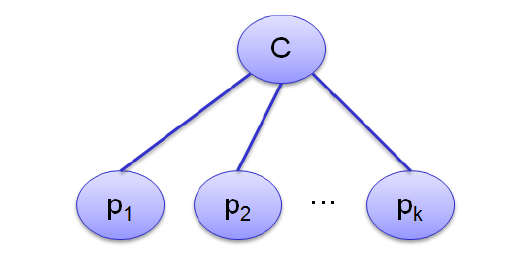
\includegraphics[width=10cm]{3_2.png}
\end{figure}
\section{قرینه‌سازی}
قرینه‌سازی\footnote{Symmetrization} یک تکنیک برای یافتن کمینه در بازی‌های $k$-نفره است.\cite{zhang11} به طور خلاصه، این روش شامل کاهش پروتکل $f_{k}(x_{1},x_{2},...,x_{k})$ به پروتکل   $f_{2}(x,y)$ است. هدف از این تکنیک این است که نشان دهیم محاسبه $f_{k}$ حداکثر به اندازه $k$ برابر $f_{2}$ است. در این مدل، توجه ما روی یک مدل هماهنگ‌کننده با وضعیت تصادفی سکه عمومی\footnote{Public Coin Randomization} است. 

\subsection{تکنیک}
با توجه به یک پروتکل $P_{k}$ که تابع  $f_{k}$ را محاسبه می‌کند، یک پروتکل $P_{2}$ که تابع $f_{2}$ را محاسبه می‌کند می‌سازیم. در مرحله اول باید یک توزیع سخت\footnote{Hard Distribution} از ورودی‌های $f_{2}$ داشته باشیم. آلیس و باب، با استفاده از این توزیع، $k$ ورودی $I_{1}, I_{2}, ..., I_{k}$ را بسازد. به هر $k$ ورودی که از آن توزیع سخت استخراج شده است، قرینه گفته می‌شود اگر هر دوتای آنها را بتوان با هم جابه جا کرد بدون آن که توزیع را عوض کنیم. در این مرحله، آلیس و باب با استفاده از این $k$ ورودی، پروتکل $P_{k}$ را محاسبه می‌کنند. 

\textbf{شبیه‌سازی.} 
آلیس یکی از بازیکنان را به صورت رندوم انتخاب می‌کند. چون وضعیت تصادفی عمومی است، باب می‌د‌‌اند که آلیس کدام بازیکن را انتخاب کرده‌است پس او بقیه بازیکنان را برمی‌د‌ارد و سپس هر دو رفتار بازیکنان را شبیه‌سازی می‌کنند. فرض کنید که آلیس بازیکن $P_{i}$ را انتخاب کرده‌است. در در نتیجه هر پیغامی که بین بازیکن $i$م و بقیه بازیکنان رد و بدل می‌شود، بین آلیس و باب هم رد و بدل می‌شود. بقیه پیغام‌ها در این مدل به عنوان پیچیدگی ارتباطی حساب نمی‌شوند. 
 
 
\textbf{کمینه.}
 هزینه پروتکل $P_{2}$ را  $Cost(P_{2})$ و هزینه پروتکل $P_{k}$ را $Cost(P_{k})$ بنامید. از آنجایی که ورود‌ی‌ها قرینه هستند، از نظر امید ریاضی، $P_{2}$ حداکثر $1/k$ کل بیت‌هایی را مخابره می‌کند که $P_{k}$ می‌کرده است. این بدین علت است که به صورت یکنواخت، امکان انتخاب هر بازیکن دیگر برای آلیس وجود داشت، در نتیجه امید ریاضی یالی که آلیس در مدل گرافی معادل انتخاب کرده‌است، $1/k$ کل یال‌ها اطلاعات رد و بدل می‌کرده است. در نتیجه
\begin{equation}
	{E}[Cost(P_{2})] \leq (1/k) {E}[Cost(P_{k})]
\end{equation}
\begin{figure}[h]
	\caption{شبیه‌سازی مدل -$k$تایی}
	\centering
	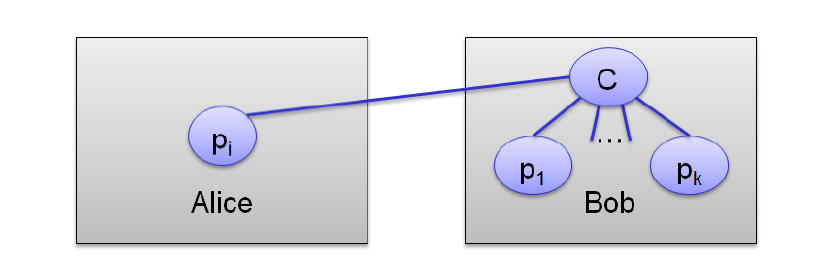
\includegraphics[width=10cm]{3_3.png}
\end{figure}
\subsection{پیشنیازها} %TODO Better title
همانطور که در \autoref{dist_rand} بیان شد، پیچیدگی ارتباطی توزیعی \footnote{Distributional communication complexity} $D_{\epsilon}^{\mu}$ با خطای $\epsilon$ و توزیع ورودی $\mu$ به صورت زیر تعریف می‌شود:
\begin{equation}
	D_{\epsilon}^{\mu} = \min_{P} \max_{x} Cost(P(x))\mu (x)
\end{equation}
در حالی که $Cost(P(x))$ هزینه پروتکل $P$ بر روی ورودی $x$ است. به عبارتی دیگر، $D_{\epsilon}^{\mu}$ بدترین حالت مخابره برای یک ورودی (بدترین ورودی) برای بهترین پروتکل است. 

از آنجایی که مخابره $k$-نفره $k$ برابر امید مخابره 2 نفره است، مفهومی از امید باید در پیچیدگی ارتباطی تعریف شود. امید پیچیدگی ارتباطی توزیعی ${E}[D_{\epsilon}^{\mu}]$ با خطای $\epsilon$ و توزیع $\mu$ به صورت زیر است
\begin{equation}
 {E}[D_{\epsilon}^{\mu}] = \min_{P} {E}_{x}[Cost(P(x))\mu(x)].
\end{equation}
در نتیجه این تعریف و قضیه مین‌ومکس یائو\footnote{Yao's Minmax Theorem} می‌توان گفت:
\begin{equation}
	R_{\epsilon} \geq D^{\mu}_{\epsilon} \geq {E}[D_{\epsilon}^{\mu}]
\end{equation}
حال با اتکا به قضیه نظریه اطلاعاتی زیر، تعدادی مثال مطرح می‌کنیم.\cite{zhang11}

 
{قضیه:}
 فرض کنید آلیس و باب هر کدام یک ورودی یکنواخت $n$ بیتی دارند. برای آن‌که آلیس با احتمال $(1-\epsilon)$ ورودی باب را بداند، لازم است امیداً باب $(1-\epsilon)n$ بیت بفرستد.

\section{مثال}
\subsection{$k-XOR$: هماهنگ‌کننده}
مساله $k-XOR$ در مدل هماهنگ‌کننده به صورت زیر است:
\begin{enumerate}
	\item بازیکن‌ها $p_{1},p_{2},p_{3},...,p_{k}$ هستند. 
	\item ورودی‌ها رشته‌های $n$ بیتی به صورت $I_{1},I_{2},I_{3},...,I_{k}$ هستند.
	\item خروجی یک رشته $n$ بیتی است که بیت $i$م، $XOR$ بیت $i$م ورودی‌هاست.
\end{enumerate}
هدف استفاده از پروتکل $P_{k}$ برای طراحی پروتکل $P_{2}$ است. بعد از آن، از کمینه پروتکل $2-XOR$ استفاده می‌کنیم تا یک کمینه روی مخابره $k$-نفره بیابیم. 

\textbf{ساخت ورودی‌های قرینه برای $P_{k}$:} 
اول از همه باید یک توزیع سخت برای ورودی مخابره دونفره پیدا کنیم که به اندازه کافی برای یافت کمینه این مخابره سخت باشد. برای این کار توزیع یکنواخت به اندازه کافی سخت است. در نتیجه، آلیس به صورت یکنواخت تصادفی  بازیکن $p_{i}$ را انتخاب می‌کند و $I_{i}$ را برابر با ورودی خودش یعنی $x$ قرار می‌دهد. باب نیز به صورت تصادفی $k-1$ رشته $n$ بیتی را به صورتی می‌سازد که 
\begin{equation}
	\{I_{j} \, | \, j \ne i \} \quad s.t. \, \, XOR(I_{1},I_{2},...,I_{i-1},I_{i+1},...,I_{k}) = y
\end{equation}
که در آن $y$ ورودی باب است. ورودی‌ها به وضوح قرینه هستند. آلیس بازیکن $i$م و باب همه $k-1$ بازیکن دیگر و همینطور هماهنگ‌کننده را شبیه‌سازی می‌کند.

\textbf{کمینه:}
از آنجایی که ورودی‌ها قرینه هستند، امید مقدار مخابره بین $p_{i}$ و هماهنگ‌کننده $1/k$ برابر کل مخابره پروتکل $P_{k}$ است. در نتیحه، $Cost(P_{2}) \leq (1/k)E[Cost(P_{k})]$ است و یا $Cost(P_{k}) \geq kE[Cost(P_{2)}]$. حال لازم است یک کمینه برای $kE[Cost(P_{2)}]$ بیابیم. 

با داشتن $XOR(x,y)$، آلیس می‌تواند ورودی باب یعنی $y$ را بازیابی کند. طبق قضیه نظریه اطلاعاتی، باب باید امیداً $n$ بیت بفرستد که یعنی $kE[Cost(P_{2})] \geq n$ و در نتیجه، $Cost(P_{k}) \geq nk$.    
\subsection{$k-XOR$: تخته‌سیاه}
مساله مثال قبل را در نظر بگیرید. مدل ارتباطی را به مدل تخته‌سیاه عوض کنید. ساخت ورودی‌ها و شبیه‌سازی با تغییر مدل نیز تغییر می‌یابند. 

\textbf{آماده‌سازی شبیه‌سازی:} 
آلیس و باب هرکدام به صورت یکنواخت تصادفی بازیکن $p_{i}$ و $p_{j}$ را انتخاب می‌کنند ($i \ne j $). آلیس همه‌ بازیکن‌ها به جز بازیکن $j$ را شبیه‌سازی می‌کند. همینطور باب، همه بازیکن‌ها به جز بازیکن $i$ را شبیه‌سازی می‌کند. در نتیجه، هر بازیکنی به جز $i$ و $j$ توسط هر دو طرف شبیه‌سازی می‌شود. 
\begin{figure}[h]
	\caption{شبیه‌سازی دوتایی آلیس و باب برای پروتکل $k$تایی $k-XOR$ در مدل تخته‌سیاه}
	\centering
	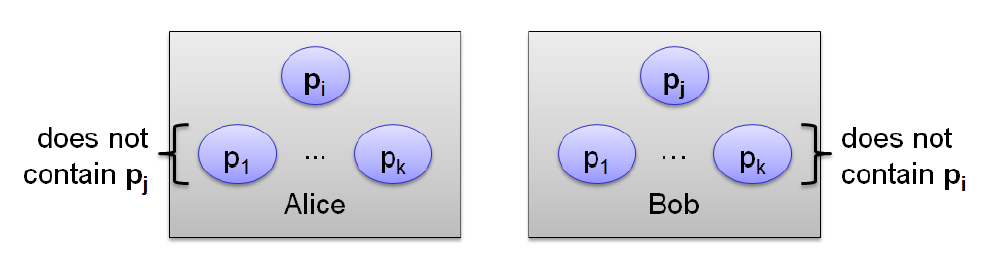
\includegraphics[width=10cm]{3_4.png}
\end{figure}

\textbf{ساخت ورودی قرینه}
مانند حالت قبل، توزیع یکنواخت یک توزیع سخت محسوب می‌شود. آلیس مقدار $I_{i}$ را برابر با $x$ قرار می‌دهد. باب نیز مقدار $I_{j}$ را برابر با $y$ قرار می‌دهد. بقیه ورودی‌ها به صورت تصادفی با استفاده از سکه عمومی مشترک مقداردهی می‌شوند. مشخص است که ورودی‌های ساخته شده قرینه هستند. 

\textbf{اجرای شبیه‌سازی:}
هربار بازیکن $i$م بیتی را روی تخته می‌نویسد، بقیه افراد باید مقدار نوشته شده را بتوانند بخوانند. اما از آنجایی که باب $p_{i}$ را شبیه سازی نمی‌کند، تا زمانی که آلیس همان‌چیزی که $p_{i}$ می‌نویسد را روی تخته‌‌سیاه ننویسید، یک بازیکن مانند $p_{j}$ از مخابرات $p_{i}$ آگاه نمی‌شود. پس هرگاه در پروتکل $P_{k}$، $p_{i}$ اطلاعاتی را مخابره کند، آلیس نیز باید آن‌ را مخابره کند. این مساله برای باب و بازیکن $p_{j}$ نیز صادق است. ولی مخابرات بقیه بازیکنان نیازی به نوشته شدن روی تخته‌سیاه ندارد چرا که هر دو طرف آن‌ها را شبیه‌سازی می‌کنند. 

 \textbf{پیچیدگی ارتباطی:} 
 از آنجایی که ورودی‌ها قرینه هستند و آلیس و باب تنها زمانی مخابره می‌کنند که دوتا از بازیکنان مخابره می‌کنند، امید مقدار مخابره برای $P_{2}$ حداکثر $\frac{k}{2}$ برابر مخابره برای $P_{k}$ است. در نتیجه، $E[Cost(P_{2})] \leq (2\k)Cost(P_{k})$ است که برابر است با $Cost(P_{k}) \geq (k/2)E[Cost(P_{2})]$. طبق قضیه نظریه اطلاعات، $E[Cost(P_{2})] = n$. در نهایت، $Cost(P_{k}) \geq \frac{nk}{2}$.
\subsection{$k-DISJ$ بدون قرینه‌سازی}
مساله اشتراک\footnote{Disjointness} به صورت گسترده در مخابرات دوتایی استفاده شده‌است و بسیاری از مسائل به این مساله کاهش یافته‌اند. این درحالی است که نسخه $k$-تایی این مساله، یعنی مساله‌ای که $k$ بازیکن خروجی 1 می‌دهند اگر و تنها اگر همه بازیکنان در یک عضو اشتراک داشته باشند، این خاصیت را ندارد. برای این که این مساله را نشان دهیم، یک پروتکل با پیچیدگی $O(nk)$ طراحی می‌کنیم. درنهایت مساله‌ای را معرفی می‌کنیم که کمینه بیشتری دارد. \cite{arkadev14} 

در مرحله اول، همه بازیکنان درخت پوشای کمینه گراف ارتباطی را به صورت محلی محاسبه می‌کنند. یک بازیکن دلخواه مانند $p_{root}$ را به عنوان ریشه درخت در نظر بگیرید. هر بازیکنی که برگ است، ورودی خود را به پدر خود می‌فرستد. پدر، اشتراک مجموعه خود و فرزندانش را محاسبه می‌کند و برای پدر خود می‌فرستد. این درخت پوشای کمینه دقیقا $k-1$ یال دارد که هر کدام $n$ بیت داده جابه‌جا می‌کنند. در پایان پروتکل، $p_{root}$ اشتراک همه را می‌داند و می‌تواند خروجی را به همه اطلاع دهد. پیچیدگی ارتباطی این پروتکل، $(k-1)(n+1)$ است.  

حال مساله‌ای مانند $k-DIST$، که در آن بازیکنان خروجی $1$ می‌دهند اگر و تنها اگر هردوتایی از ورودی‌ها متمایز باشد، در نظر بگیرید. می‌توان نشان داد که پروتکل بهینه برای این مساله وقتی است که همه بازیکنان ورودی‌شان را برای یک دیگر می‌فرستند. در یک گراف ارتباطی با قطر $d$، یعنی بلندترین کوتاه‌ترین مسیر، تعداد مخابره مورد نیاز برای آگاه شدن همه از ورودی یک‌دیگر برابر با $O(nkd)$ است. اگر گراف کامل باشد، $d$ برابر با $1$ است و بزگترین مقدار می‌تواند $k$ باشد که کمینه $O(nk^{2})$ را می‌دهد. 

 از دیگر مسائل سخت می‌توان به مسائلی اشاره کرد که در یک مخابره $k$تایی، هر بازیکن یک زیرگراف مانند $H_{k}$ از یک گراف مانند $G$ را داشته باشند و بخواهند تصمیم بگیرند که درجه یک راس مشخص در $G$ چند است، آیا $G$ دور دارد یا خیر، مثلث دارد یا خیر، متصل است یا خیر و آیا دوبخشی است یا خیر. \cite{arkadev14}
 
\chapter{کاربرد پیچیدگی ارتباطی در ساختمان داده‌ها }\label{chapter4}
در این بخش از گزارش، در مورد استفاده از پیچیدگی ارتباطی برای یافتن کمینه‌ها در حوزه ساختمان‌ داده‌ها می‌پردازیم. برای شروع، تعریفی بر روی مدل جست‌وجوی سلول خواهیم داشت، ساختمان‌ داده‌های ایستا و پویا را تعریف می‌کنیم و ارتباط پیچیدگی ارتباطی نامتقارن و مدل جست‌وجوی سلول را مطرح می‌کنیم. در ادامه، با معرفی تکنیک‌ حریصانه در پیچیدگی ارتباطی، کمینه‌های ساختمان داده‌ای را به پیچیدگی مخابرات نزدیک می‌کنیم. 


\section{مدل جست‌وجوی سلول}
می‌توانید مدل جست‌جوی سلول\footnote{Cell Probe} را یک پردازنده و یک حافظه دسترسی تصادفی در نظر بگیرید. یک ساختمان داده را فرض کنید که در این حافظه ذخیره شده است و پردازنده باید با استفاده از این داده به یک جست‌وجو پاسخ دهد. برای ادامه بحث، $s$ تعداد خانه‌های حافظه و $w$ تعداد بیت‌ در هر خانه است. پیچیدگی کار یه تعداد خانه‌هایی است که پردازنده در حین پاسخ به جست‌وجو به آن‌ها دسترسی می‌یابد.\cite{ajtai88} 

این مدل، اصلی‌ترین مدل برای اثبات کمینه‌ها در ساختمان داده‌هاست. این بدین معناست که کمینه‌های این مدل، کمینه‌های مدل‌های دیگر را در بر دارد. این موضوع برای بیشینه‌ها نیز صادق است. 

\begin{definition}
یک مساله ساختمان داده ایستا، مساله‌ای است که با توجه به یک $map$ مانند $f:Q\times D \rightarrow A$ است که در آن $D$ یک مجموعه از داده‌ها است، $Q$ یک مجموعه از جست‌وجوهاست و $f(q,d)$ پاسخ به جست‌وچوی $q$ در مورد داده ‏$d$ است. $A$ نیز مجموعه همه پاسخ‌هاست. 
\end{definition}

\begin{definition}
پاسخ به یک مساله ساختمان داده ایستا در مدل جست‌وجوی سلول با پارامترهای $s$ و $w$ و $t$، یک روش برای کدگذاری هر داده مانند $d \in D$ در حافظه ماشین است در صورتی که از $s$ خانه حافظه با $w$ بیت استفاده کنیم در حالی که حداکثر لازم است $t$ خانه را بررسی کنیم تا بتوانیم پاسخی بیابیم. 
\end{definition}

\begin{example}
با در دست داشتن یک مجموعه مرتب مانند $U = \{ 1,...,m\}$ و یک زیر مجموعه مانند $S \subseteq U$، به نحوی $S$ را کدگذاری کنیم و در حافظه قرار دهیم که بتوانیم اولین نیاکان یک عضو مانند $x \in U$ را در $S$ بیابیم. 
\end{example}
 
\begin{definition}
ساختمان داده‌های پویا:
ساختمان داده‌های پویا شباهت زیادی به ساختمان‌داده‌های ایستا دارند به جز آن‌که در این مسائل باید بتوان داده‌ها به صورت بهینه در ساختمان‌ داده ذخیره کرد.
\end{definition}


\section{پیچیدگی ارتباطی نامتقارن}

در این مساله، با پیچیدگی ارتباطی قطعی سروکار داریم. می‌توان هر مساله ساختمان داده را به یک مخابره تبدیل کرد: آلیس یک جست‌وجو مانند $q \in Q$ دریافت می‌کند. و باب یک داده $d \in D$ را دریافت می‌کند و هردو تلاش می‌کند که تابع $f(q,d)$ را محاسبه کنند.\cite{Nisan98} البته بین این مدل و مدل اصلی مخابره تفاوتی وجود دارد. مثلا، اندازه داده خیلی بیشتر از جست‌وجو است در نتیجه مخابرات به صورتی نامقارن است، یعنی بار ارتباطی سمتی از مخابره همواره بیشتر از سمتی دیگر است.  همچنین تنها آلیس نیاز دارد که پاسخ را بداند. در ادامه، پیچیدگی ارتباطی این مدل باید به طور دیگری سنجیده شود. آلیس پیغام خود را از مجموعه $\{1,...,s\}$ انتخاب می‌کند و باب پیغام خود را از بین $\{1,...,2^{w}-1\}$ انتخاب می‌کند. پیچیدگی پروتکل همان ماکسیمم تعداد دورهای مخابره بین آلیس و باب است. به صورت رسمی:

\begin{definition}
می‌گوییم یک پروتکل مانند $P$، یک $[t,(a,b)]^{A}$-پروتکل برای تابع $f$ است اگر همه پیام‌های آلیس حداکثر $a$  بیت باشد و پیغام‌های باب حداکثر $b$ بیت باشد و حداکثر $t$ دور مخابره انجام شود در حالی که مخابره را آلیس شروع کرده است. یک $[t,(a,b)]^{B}$-پروتکل به همین صورت تعریف می‌شود با تفاوت آن‌که باب مخابره را شروع می‌کند.  
\end{definition}

\begin{theorem}
اگر یک پاسخ به مساله جست‌وجوی سلول از $s$ خانه استفاده کند و حداکثر شامل $t$ بار دسترسی به خانه‌های حافظه باشد، یک $[t,(\log s,w)]^{A}$-پروتکل برای مساله متناظر معادل وجود دارد. 
\end{theorem}

اثبات شبیه‌سازی مطرح شده در تعریف است. \\

از قضینه بالا می‌توان نتیجه گرفت برای آن که بتوانیم یک کمینه مانند $\Omega(f)$ برای یک مساله ایستا ثابت کنیم (فرض می‌کنیم که $s \in O(n)$) باید نشان دهیم که هیچ یک $[o(f),(\log n,w)]^{A}$-پروتکلی برای مساله ارتباطی معادلش وجود ندارد. 
 

در مرحله بعد، نشان می‌دهیم که یک مساله ایستا می‌تواند به یک مساله پویا کاهش یابد.


\begin{definition}
مساله ساختمان داده ایستا $f$ متناظر با مساله پویا $g$ به این صورت تعریف می‌شود: برای یک پارامتر $d$، $f: Q \times D \rightarrow A$ تابع ایستای ماست که $Q$ همان جست‌وجوهای مساله پویا است و $D$ تمامی حالت‌های قابل دسترسی از حالت اولیه است که حداکثر $d$ بار تغییر یافتن بر روی آن رخ داده‌است.
\end{definition}

\begin{theorem}
اگر یک پاسخ مساله جست‌وجوی سلول از $n^{O(1)}$ خانه حافظه استفاده کند و $t$ بار دسترسی به حافظه انجام دهد برای تابع $g$ که یک مساله پویاست، در نتیجه مساله معادل ایستای $f$ یک پاسخ دارد که از $O(dt)$ خانه حافظه استفاده می‌کند و $O(t)$ دسترسی انجام می‌دهد. 

\end{theorem}

\begin{proof}
پاسخ ایستا به صورت ساده پاسخ پویا را شبیه‌سازی می‌کند. فرض کنید که ساختمان داده مساله پویا به نحوی در حافظه کدگذاری شده‌است که به طوری که حالت اولیه همه خانه‌ها برابر با $0$ هستند. در پاسخ مساله ایستا، به جای ذخیره مقادیر خانه‌هایی که پاسخ پویا به آن‌ها دسترسی داشته است در جای خودشان، همه خانه‌هایی که مقدارشان تغییر کرده است را به همراه مقدار نهایی‌شان در یک دیکشنری قرار می‌دهیم، این عملیات در فضای $O(dt)$ امکان‌پذیر است. هر بار که پاسخ پویا می‌خواهد به یک خانه به‌خصوص دسترسی داشته باشد، ابتدا چک می‌کنیم که آن‌ خانه در دیکشنری وجود دارد یا خیر. اگر داشت، مقدار نهایی را برمی‌گردانیم، در غیر این صورت، $0$ برمی‌گردانیم. هر جست‌وجو $O(1)$ زمان می‌برد و نهایتا باید $O(t)$ جست‌وجو بزنیم. 
\end{proof}

در نتیجه دیدیم که کمینه برای یک پروتکل مخابره، یک کمینه برای مساله ساختمان داده ایستا است؛ همچنین، هر کمینه برای ساختمان داده ایستا، یک کمینه برای ساختمان داده پویا است. از آنجایی که در پروتکل مخابره، آلیس می‌تواند کل ورودی را برای باب بفرستد، بهترین کمینه‌ای که می‌توانیم با استفاده از این مدل از کاهش به پیچیدگی ارتباطی برای مسائل ساختمان داده به دست آوریم برابر است با $t = \Omega(\frac{\log |Q|}{\log s} )$ اگر تعداد جست‌وجوها یک چندجمله‌ای در $n$ باشد، کمینه یک مقدار ثابت خواهد بود. به همین علت، تنها مسائلی که حداقل در $n$ نمایی باشند در نظر می‌گیریم. 

\section{ کمینه}

تکنیک‌های اصلی اثبات کمینه برای مدل جست‌وجوی سلولی با استفاده از پیچیدگی ارتباطی استفاده از حذف دور\footnote{Round Elimination}، تکنیک غنا\footnote{Richness Technique}، تکنیک پیچیدگی ارتباطی حریصانه\footnote{Greedy CC Technique} و کاهش به مساله اشتراک است. در اینجا به بررسی  تکنیک حریصانه می‌پردازیم. \cite{Nisan98}

\subsection{تکنیک پیچیدگی ارتباطی حریصانه}
\begin{definition}
\textbf{شرط ردیف تک‌رنگ\footnote{Monochromatic Row}:}
یک تابع مانند $h:A\times B \rightarrow C$ را در نظر بگیرید. $A^{'} \subseteq A$ و $B^{'} \subseteq B$ شرط ردیف تک‌رنگ را ارضا می‌کنند اگر:
\begin{equation}
	\forall x \in A^{'}, \forall y,z \in B^{'}: h(x,y) = h(x,z).
\end{equation}
\end{definition}
ایده اصلی آن است که با توجه به ماتریس مخابره آلیس و باب، نشان دهیم که همه مستطیل‌هایی که شرط ردیف تک‌رنگ را ارضا می‌کنند، کوچک هستند و تا بتوانیم قضیه بعد را اعمال کنیم و یک کمینه برای تعداد دورهای مکالمه به دست آوریم. از این به بعد، به مستطیل‌هایی که شرط ردیف تک‌رنگ را ارضا کند، مستطیل خوب می‌گوییم. 

یک مساله مخابره مانند $h:A\times B \rightarrow C$ را در نظر بگیرید. آلیس ورودی $ a \in A$ و باب ورودی $b \in B$ را دارد و بنا است که مقدار $h(a,b)$ محاسبه شود. همچنین، آلیس پیام‌های خود را از مجموعه $\{1,...,s\}$ انتخاب می‌کند و باب پیام‌های خود را از مجموعه $\{1,...,k\}$ انتخاب می‌کند. 

\begin{theorem}
 اگر $h$ یک پروتکل $t$ دوری داشته باشد، یک $A^{'} \subseteq A$ و $B^{'} \subseteq B$ وجود دارد به طوری که $|A^{'}| \geq |A|/s^{t}$ و $|B^{'}| \geq |B|/k^{t}$ و  $A^{'}$ و $B^{'}$ که شرط ردیف تک‌رنگی را ارضا می‌کنند.
\end{theorem}
 
\begin{proof}
 استقرا روی $t$. برای حکم پایه، $t = 0$ در نظر بگیرید. چون هیچ مخابره‌ای انجام نمی‌شود، خروجی فقط به ورودی آلیس وابسته است، پس همه ردیف‌های باید تک‌رنگی باشند تا جوابی برای پروتکل داشته باشیم. در این‌ صورت، $A^{'} = A$ و $B^{'} = B$. 
 
 حال فرض کنید قضیه برای $t = k$ درست باشد. یک مساله ارتباطی با یک پروتکل $t+1$ دوری در نظر بگیرید. 
 برای هر  $a \in \{ 1,...,s\}$، تعریف کنید $A_{a}$ را از ورودی‌هایی مانند $x \in A$ که برای آن‌ها آلیس در ابتدا $a$ را ارسال می‌کرده است. 
 با توجه به اصل لانه کبوتری، می‌توانیم $a$ را به نحوی ثابت نگه داریم  که $|A_{a}| \geq |A|/s$. 
 همین‌طور،  تعریف کنید $B_{b}$ را از ورودی‌هایی مانند $x \in B $ که برای آن‌ها باب در ابتدا $b$ را ارسال می‌کرده است. 
 با توجه به اصل لانه کبوتری، می‌توانیم $b$ را به نحوی ثابت نگه داریم که $|B_{b}| \geq |B|/k$. 
 یک پروتکل $t$ دوری $P^{'}$ برای مساله ارتباطی محدود به $A_{a} \times B_{b}$ وجود دارد که همان پروتکل $P$ را از مرحله دوم به بعد شبیه‌سازی می‌کند. 
 با توجه به فرض استقرا، وجود دارد یک مستطیل ساخته شده از $A_{a}^{'} \times B_{b}^{'}$ به طوری که سایزشان حداقل برابر با $1/s^{t}$ و $1/k^{t}$ برابر $A_{a}$ و $B_{b}$ است. 
 در نتیجه، برابر قراردادن $A^{'} = A^{'}_{a}$ و $B^{'} = B_{b}^{'}$ جواب دلخواه را به ما می‌دهد. 
\end{proof}

\begin{example}
 کمینه  $\Omega(n)$ برای مساله پویای ارزیابی چندجمله‌ای: ساختمان داده $y \in F^{n+1}$ ضرایب یک چندجمله‌ای است و جست‌وجوی مرتبط $x \in F^{1}$ است. پاسخ آن مشخص می‌کند که آیا این نقطه عضو جندجمله‌ای است یا خیر.

 پاسخ بدیهی این  سوال $t \in O(n)$ است. برای این که این را نشان‌دهیم، لازم است یک کمینه برای مساله ارتباطی معادل آن بیابیم. 
 
 فرض کنید که باب یک چندجمله‌ای $f$ از درجه $n$ دریافت می‌کند ($y \in F^{n+1}$). 
 همچنین آلیس یک $x\in F$ دریافت می‌کند.
  هدف این مخابره، محاسبه $f(x)$ است. 
  آلیس پیام‌های خود را از مجموعه $\{1,...,s\}$ و باب پیام‌های خود را از مجموعه $\{1,...,|F|\}$ انتخاب می‌کند. 
  حالتی را فرض کنید که $F \geq 2^{n \log n}$. 
 
 حال با استفاده از ویژگی‌های چند جمله‌ای‌ها، مشخص می‌کنیم چگونه سایز مستطیل‌های خوب باید کوچک باشد. برای هر دو چندجمله‌ای متفاوت از درجه $n$، حداکثر در $n$ نقطه با هم اشتراک دارند. پس برای یک مستطیل خوب 
 $A^{'} \times B^{'}$، $|A^{'}| \leq n$ یا $|B^{'}|\leq 1$.  حال می‌خواهیم قضیه را اعمال کنیم. 
 
 اگر $|A^{'}| \leq n$، در نتیجه $n \geq |F|/s^{t}$ در نتیجه $t \geq (\log |F| - \log n) / (\log s) \in \Omega(n)$. اگر $|B^{'}| \leq 1$، پس $1 \geq (|F|^{n+1})/ |F|^{t})$. در نتیجه $t \geq n+1$ و $t \in \Omega(n)$. 
 همین پروتکل را برای حالت خاص مساله $DISJ$ در نظر بگیرید که در آن آلیس یک عضو دارد و باب یک زیرمجموعه $l$ عضوی. آلیس مجموعه پیغام‌های خود را از مجموعه $\{0,1\}^{l\log{n}}$ انتخاب می‌کند. کافی است نشان دهیم بهترین حالت این که آلیس کل ورودی را بفرستد. اگر اندازه مجموعه‌ای که آلیس از آن انتخاب می‌کند برابر با $N = 2^{n}$ باشد، ورودی آلیس $n$ بیتی و ورودی باب $N$  بیتی خواهد بود. برای یافتن مستطیل خوب لازم است توجه کنیم که دو زیر مجموعه متفاوت $l$ تایی از $N$، حداکثر در $l-1$ عضو اشتراک دارند. پس طبق حالت قبل، سایز مستطیل خوب محدود و پیچیدگی ارتباطی برابر با $n$ خواهد بود.
  \end{example}
%\section{پیوست: مبانی ریاضی مکانیک کوانتومی}\label{chapter7}
دراین بخش با ریاضیات مورد نیاز برای فهم چارچوب نظری مکانیک کوانتومی آشنا می‌شویم.
  \subsection{فضای برداری}
  مجموعه $V$ را یک فضای برداری روی میدان $F$ می‌گوییم هرگاه دو عمل زیر تعریف شده 
  \begin{equation}
  	+ : V \times V \rightarrow V \quad , \quad . : F \times V \rightarrow V
  \end{equation}
  و دارای خواص زیر باشند: 
   \begin{equation}
   \begin{split}
   A_{1}: & \quad x + y = y + x\\
   A_{2}: & \quad (x + y) + z = x + (y + z)\\
   A_{3}: & \quad \exists 0 \in V | 0 + x = x\\
   A_{4}: & \quad \forall x \in V | -x + x = 0\\
   M_{1}: & \quad \alpha(x+y) = \alpha x + \alpha y\\
   M_{2}: & \quad (\alpha + \beta)x = \alpha x + \beta x\\
   M_{3}: & \quad \alpha(\beta x) = (\alpha\beta) x\\
   M_{4}: & \quad 1x = x
   \end{split}
   \end{equation}
   بسته به این که $F$ میدان اعداد حقیقی یا میدان اعداد مختلط باشد، فضای برداری $V$ را فضای برداری مختلط یا حقیقی گوییم. ازاین به بعد منحصراً با فضاهای برداری مختلط کار می‌کنیم. 
   
\begin{example}
مجموعه‌های زیر هرکدام یک فضای برداری هستند. 
\begin{enumerate}
	\item $R^{n}$ یا مجموعه $n$-تایی‌های مرتب حقیقی
	\item $C^{n}$ یا مجموعه $n$-تایی‌های مرتب مختلط
	\item $M_{m \times n}(F)$ یا مجموعه ماتریس‌های $m \times n$ که درایه‌های آن عناصر یک میدان $F$ هستند.
	\item $P_{n}([a,b])$ یا مجموعه چندجمله‌ای‌های حقیقی مرتبه $n$ از متغیر $x$ که در فاصله $[a,b]$ تعریف شده‌اند. 
	\item $C^{k}[a,b]$ یا مجموعه توابع حقیقی یا مختلط $k$ بار مشتق‌پذیر در بازه $[a,b]$.
\end{enumerate}  
\end{example} 
   
\begin{definition}
   هرگاه $V$ یک فضای برداری و $W \subset V$ یک زیر مجموعه از آن باشد، آنگاه $W$ را یک زیرفضای $V$ گوییم اگر $W$ نسبت به جمع بردارها و ضرب اعداد در بردارها بسته باشد. 
   \end{definition}
   
   \subsection{ضرب داخلی و اندازه}
    \textbf{تعریف:}
    در یک فضای برداری $V$ یک عمل دوتایی $\langle,\rangle : V \times V \rightarrow C$ را یک ضرب داخلی می‌نامیم هرگاه در شرایط زیر صدق کند:
    \begin{equation}
    	\langle x , y + \alpha z \rangle = \langle x , y \rangle + \alpha \langle x , z \rangle
    \end{equation}
    
    \begin{equation}
    	\langle x , y \rangle = \langle y , x \rangle^{*}
    \end{equation}
    \begin{equation}
    	\langle x , x \rangle \geq 0
    \end{equation}
    \begin{equation}
    	\langle x , x \rangle =  0 \rightarrow x = 0
    \end{equation}
    فضایی را که به ضرب داخلی مجهز شده باشد یک فضای برداری ضرب داخلی می‌گوییم. 
    \begin{theorem}
    کوشی-شوارتز:
     در فضای ضرب داخلی داریم:
\begin{equation}
 	|\langle x,y \rangle | = \langle x,x \rangle \langle y,y \rangle .
 \end{equation}
    \end{theorem}

\begin{definition}{اندازه یک بردار: }
در هر فضای ضرب داخلی، می‌توان اندازه یک بردار را به شکل زیر تعریف کرد:
\begin{equation}
	|x| := \sqrt{\langle x,x \rangle}
\end{equation}
\end{definition}
با توجه به نامساوی کوشی-شوارتز می‌توان نوشت:
\begin{equation}
	 	|\langle x,y \rangle | = |x||y|
\end{equation}


\begin{definition}{فضای نرم یا اندازه‌دار: }
یک فضای برداری $V$ که در آن نگاشت $\| \quad \| : V \rightarrow R$ تعریف شده باشد را فضای برداری اندازه‌دار\footnote{Normed Vector Space} می‌گوییم هرگاه شرایط زیر برقرار باشد:
\begin{equation}
	\| v \| \geq 0 \quad \forall v
\end{equation}
\begin{equation}
	\| v \| = 0 \rightarrow v = 0
\end{equation}
\begin{equation}
	\| \alpha v \| = |a| \|v \|
\end{equation}
\begin{equation}
\| v + w \| \leq \| v \| + \| w \|
\end{equation}
\end{definition}
هرفضای ضرب داخلی باهمان اندازه‌ای که از روی ضرب داخلی تعریف می‌شود یک فضای اندازه‌دار است، ولی یک فضای اندازه‌دار الزاماً یک فضای ضرب داخلی نیست. به عبارت دیگر، اندازه لزوما از روی ضرب داخلی تعریف نشده است. برای مثال، برای فضای توابع $C[a,b]$ نگاشت $\| f \| = sup_{x \in [a,b]} | f(x)|$ یک اندازه است که از روی ضرایب داخلی تعریف نشده‌ است. 

\subsection{پایه}
پایه به‌هنجار\footnote{Normal} $\{ e_{i}, i = 1,...,N\}$ را برای فضای برداری $V$ در نظر می‌گیریم. به‌هنجار بودن به معنای آن است که $\langle e_{i},e_{j} \rangle = \delta_{ij}$. هر بردار $x \in V$  را می‌توان بر حسب این بردار‌های پایه بسط داد و نوشت:
\begin{equation}
	x = \sum_{i = 1} ^{N} x_{i}e_{i}
\end{equation}
بدیهی است که 
\begin{equation}
	x_{i} = \langle e_{i},x \rangle
\end{equation}


پایه‌ها را می‌توان با یک ماتریس تبدیل پایه دو بعدی مانند $S$ به یک دیگر تبدیل کرد. برای مثال، فرض کنید که بردار $x$ را که در پایه $e_{i}$ است را می‌خواهیم در پایه $e^{'}_{i}$ بنویسیم. لازم است درایه‌های ماتریسی آن را استخراج کنیم. در نظر بگیرید $e^{'}_{i} = S_{li}e_{l}$:
\begin{equation}
x^{'}_{i} = \langle e^{'}_{i},x \rangle = \langle S_{li}e_{l}, x \rangle = S_{li}x_{l}
\end{equation}
و یا به صورت فشرده‌تر:
\begin{equation}
	x^{'} = xS.
\end{equation}
از آنجا که پایه‌های $\{e_{i}\}$ و $\{e^{'}_{i}\}$ هر دو بهنجار هستند به راحتی نتیجه می‌گیریم که ماتریس تبدیل پایه $S$ در شرط زیر صدق می‌کند:
\begin{equation}
S^{\dagger}S = I
\end{equation}
چنین ماتریسی را ماتریس‌های یکانی\footnote{Unitary} می‌گوییم.

که در آن $S^{\dagger}$ ماتریس الحاقی\footnote{Conjugate Transpose} $S$ است و چنین تعریف می‌شود:

\begin{equation}
S^{\dagger} = (S^{*})^{T} \quad or \quad S^{\dagger}_{ij} = (S^{*})_{ji}
\end{equation}
همچنین هرگاه ماتریس با الحاقی خود برابر باشد، آن را ماتریس هرمیتی می‌گوییم: 
\begin{equation}
	S^{\dagger} = S.
\end{equation}
%TODO example??

\subsection{فضای کامل و هیلبرت}
\begin{definition}{دنباله کوشی:}
در یک فضای برداری، دنباله‌ای از بردارها مانند $\{x_{1},x_{2},...,x_{n},...\}$  درنظر می‌گیریم. این دنباله، یک دنباله کوشی نامیده می‌شود هر گاه فاصله بین  بردارها به تدریج کم شود؛ به عبارت دقیق‌تر، هرگاه به ازای هر $\epsilon > 0$ عددی مانند $N$ یافت شود که 
\begin{equation}
	\forall m,n > N \rightarrow |x_{n} - x_{m} | \leq \epsilon
\end{equation} 
\end{definition}
در یک فضای برداری، لزوما حد کوشی در خود فضا قرار ندارد. مثلا، هرگاه میدان اعداد گویا را به عنوان یک فضای برداری روی خودش درنظر بگیریم، دنباله $\{ ( 1 + \frac{1}{n})^{n} \}$ اگرچه یک دنباله کوشی است، ولی حد آن در میان اعداد گویا قرار ندارد. با افزودن اعداد گنگ به میدان، یک فضای برداری میدان حقیقی به دست می‌آید که کامل است. 

\begin{definition}
یک فضای برداری را فضای برداری کامل گوییم هرگاه حد دنباله کوشی را در خود داشته باشد. 
\end{definition}
 
\begin{definition}
 یک فضای برداری با ضرب داخلی کامل را فضای هیلبرت\footnote{Hilbert Space}  می‌نامیم. از آنجایی که میدان اعداد حقیقی و مختلط کامل است، می‌توان ثابت کرد هر فضا با بعد محدود روی این میدان‌ها هیلبرت است. 
 \end{definition}
 
\subsection{تبدیلات خطی}
در یک فضای برداری  $V$، نگاشت 
$\hat{T} : V \rightarrow V$ را یک تبدیل خطی یا یک عملگر خطی\footnote{Linear Operator} می‌گوییم هرگاه داری خاصیت زیر باشد:
\begin{equation}
	\hat{T}(x + \alpha y ) = \hat{T}(x) + \alpha \hat{T}(y) \quad \forall \alpha \in F, x,y \in V
\end{equation}
ماتریس $T$ با درایه‌های $T_{mn}$ را ماتریس مربوط به تبدیل خطی $\hat{T}$ در پایه $\{e_{i}\}$ می‌گوییم. هرگاه پایه فوق به‌هنجار باشد، می‌توانیم بنویسیم 
\begin{equation}
	\langle e_{j}, \hat{T}e_{i} \rangle = T_{ji}
\end{equation}
تاثیر تابع $\hat{T}$ روی بردار $x$ عبارت است از:
\begin{equation}
	\hat{T}x = \hat{T}x_{i}e_{i} = x_{i}(\hat{T}e_{i}) = x_{i}T_{ji}e_{j} = (T_{ji}x_{i})e_{j} = (Tx)_{j}e_{j}
\end{equation}
که برابر با ضرب از سمت چپ ماتریس $T$ روی $x$ است. 

همچنین، با تعویض پایه، ماتریس تغییر می‌یابد:
\begin{equation}
	T^{'}_{ij} = \langle e^{'}_{i},\hat{T}e^{'}_{j} \rangle = \langle S_{li}e_{l},\hat{T}S_{mj}e_{m} \rangle = S^{*}_{li}T_{lm}S_{mj}
\end{equation}
که به صورت زیر قابل بازنویسی است:
\begin{equation}
T^{'} = S^{\dagger}TS
\end{equation}

هرگاه $A$ و $B$ دو تبدیل خطی دلخواه روی $V$ و $\alpha$ عددی دلخواه متعلق به میدان $F$ باشد، آنگاه $\alpha A+B$ نیز یک تبدیل خطی روی $V$ است. درنتیجه، مجموعه تبدیلات خطی روی $V$ تشکیل یک فضای برداری می‌دهند که آن را با $End(V)$ نشان می‌دهیم. همچنین، ضرب دو تبدیل خطی با تعریف 
\begin{equation}
	(AB)x := A(Bx)
\end{equation}
 نیز یک تبدیل خطی است. پس می‌توان گفت که $End(V)$ نه تنها یک فضای برداری است بلکه یک جبر است که خاصیت شرکت پذیری دارد ($(AB)C = A(BC)S$) ولی جبر جابه‌جایی ندارد ($AB \ne BA$) اما یکه‌دار\footnote{Unital} است که یعنی عنصری دارد مانند $I$ که $AI = IA = A$. 
 
 دیدیم که به یک عملگر خطی می‌توان یک ماتریس نسبت داد. وقتی که پایه فضا را معین می‌کنیم، بین فضای تبدیلات خطی یعنی $End(V)$ و فضای ماتریس‌های $M_{n \times n}(C)$ یک نگاشت یک به یک خواهیم داشت. بنابراین یک تبدیل خطی و ماتریس آن به جای هم قابل استفاده هستند. همچنین، با تبدیل زیر می‌توان فضای تبدیل خطی روی $V$ را به یک فضای ضرب داخلی تبدیل کرد:
  \begin{equation}
  	\langle A,B \rangle = tr(AB^{\dagger})
  \end{equation}
  که در آن رد\footnote{Trace} ماتریس $tr(A)$ برای ماتریس مربعی $A$ برابر با مجموعه درایه‌های قطر اصلی است.
  
  \subsection{جمع نیمه‌مستقیم دو زیرفضا}
  
\begin{definition}
  هرگاه $V$ یک فضای برداری و $U$ و $W$ دو زیرفضای آن باشند، $U + W$ را به عنوان مجموعه زیر تعریف می‌کنیم:
  \begin{equation}
  	U + W := \{ v | v = u + w, u \in U, w \in W \}
  \end{equation}
   واضح است که $U + W$ نیز یک زیرفضا برای $V$ است. 
   \end{definition}
 \begin{definition}
   فرض کنید که $V$ یک فضای برداری و $W$ و $U$ دو زیرفضای آن باشند به طوری که:
   \begin{enumerate}
   \item $V = W + U$
   \item تنها بردار مشترک $U$ و $W$ بردار صفر باشد. 
   \end{enumerate}
   در این صورت $V$ جمع نیمه‌مستقیم\footnote{Semi-direct Sum} $U$ و $W$ می‌گوییم و می‌نویسیم 
   \begin{equation}
   V = U \oplus W
   \end{equation}
   \end{definition}
   \begin{theorem}
   $V = W \oplus U$ اگر و تنها اگر هر بردار $v \in V$ را بتوان به صورت $u + w$ یکتایی نوشت که در آن $u \in U$  و  $w \in W$. 
   \end{theorem}
   \begin{theorem}
   اگر $V = U + W$ آنگاه $dim(V) = dim(U) + dim(W)$. 
   \end{theorem}
   \begin{definition}
   فرض کنید که $V = V_{1} \oplus V_{2} \oplus ... \oplus V_{r}$. در این صورت، هر بردار $v \in V$ به صورت یکتای $v = v_{1} + v_{2} + ... + v_{r}$ تجزیه می‌شود. $P_{j}$ را عملگری تعریف کنید که:
   \begin{equation}
   		P_{j}v = v_{j}
   \end{equation}
   در این صورت، $P_{j}$ را عملگر تصویر روی زیرفضای  $V_{j}$ می‌خوانیم. 
   \end{definition}
   \begin{theorem}
   عملگرهای تصویری\footnote{Image Operators} خواص زیر را دارند:
   \begin{enumerate}
   	\item $P_{j}P_{k} = \delta_{jk}P_{j}$
   	\item $\sum_{j=1}^{r} P_{j} = I$
   \end{enumerate}
   \end{theorem}
   \begin{theorem}
   هرگاه $V$ یک فضای ضرب داخلی باشد و $V = \bigoplus_{j=1}^{r} V_{j}$ که در آن $V_{j}$ها بر هم عمود هستند، آنگاه عملگرهای $P_{j}$ هرمیتی\footnote{Hermitian} هستند. 
   \end{theorem}
   \subsection{مساله ویژه‌مقدار}
   عملگر $T: V \rightarrow V$ را درنظر می‌گیریم. مساله ویژه‌مقدار\footnote{Eigenvalue} عبارت است از یافتن بردارهای غیرصفری که تحت اثر $T$ به مضربی از خود تبدیل بشوند: 
   \begin{equation}
   Tx = \lambda x
   \end{equation}
    بردار $x$ غیرصفر خواهد بود هرگاه ماتریس $T - \lambda I$ وارون‌پذیر نباشد، یعنی این‌که
    \begin{equation}
    	det(T-\lambda I) = 0
    \end{equation}
    این معادله، یک معادله درجه $N$ است که در حوزه اعداد مختلط حتما $N$ جواب مانند  $\{ \lambda_{i}, i = 1,...,N\} $ دارد که به آن‌ها ویژه‌مقدارهای تبدیل $T$ گوییم. این جواب‌ها لزوما با هم متفاوت نیستند. 
    
    بردار مربوط به $\lambda_{i}$ که در معادله $Tv_{i} = \lambda_{i} v_{i}$ صدق می‌کند را ویژه‌بردار\footnote{Eigenvector} متناظر با آن ویژه‌مقدار می‌خوانیم. هرگاه $x$ و $y$ ویژه‌بردارهای مربوط به $\lambda$ باشند، بدیهی است که هر ترکیب خطی از آن‌ها هم ویژه‌برداری از $\lambda$ است. بنابراین، مجموعه بردارهای متعلق به یک ویژه‌مقدار تشکیل یک زیرفضا را می‌دهند که به آن ویژه‌فضای\footnote{Eigenspace} آن ویژه‌مقدار می‌گویند. 
    
    \subsection{عملگرهای هرمیتی، یکانی و به‌هنجار}
    
    \begin{definition}
    در یک فضای ضرب داخلی، الحاقی یک عملگر $T$ عملگری مانند $T^{\dagger}$ است که در شرط زیر صدق کند: 
    \begin{equation}
    	\langle v,Tw \rangle = \langle T^{\dagger}v,w \rangle
    \end{equation}
    \end{definition}
    با استفاده از این تعریف می‌توان به راحتی خواص زیر را ثابت کرد:
    \begin{enumerate}
    	\item الحاقی یک عملگر خطی خود نیز یک عملگر خطی است.
    	\item $(cA + B)^{\dagger} = c^{*}A^{\dagger} + B^{\dagger}$
    	\item $AB)^{\dagger} = B^{\dagger}A^{\dagger}$
    	\item $(A^{\dagger})^{\dagger} = A$
    \end{enumerate}
     
      \begin{definition}
     در یک فضای ضرب داخلی عملگر هرمیتی به عملگری گفته می‌شود که در شرط $T^{\dagger} = T$ صدق کند. عملگر پادهرمیتی به عملگری گفته می‌شود که در شرط $T^{\dagger} = -T$ صدق کند. 
     \end{definition}
     \begin{definition}
     در یک فضای ضرب داخلی، عملگر یکانی $U$ به عملگری گفته می‌شود که ضرب داخلی بردارها رو حفظ کند، یعنی 
      \begin{equation}
      	\langle Uv,Uw \rangle = \langle v,w \rangle
      \end{equation}
      چنین عملگری در شرط $UU^{\dagger} = U^{\dagger}U$ صدق می‌کند. 
      \end{definition}
      \begin{definition}
      عملگر نرمال یا به‌هنجار عملگری است که با الحاقی خود جابه‌حا شود. عملگرهای هرمیتی و یکانی نرمال هستند. 
      \begin{equation}
      	AA^{\dagger} = A^{\dagger}A
      \end{equation}
      \end{definition}
      \begin{theorem}
      فرض کنید که $A$ یک عملگر به‌هنجار است. در این صورت اگر $Ax = \lambda x$ آنگاه $A^{\dagger} x = \lambda^{*} x$.
      \end{theorem}
      \textbf{نتیجه: }
      ویژه‌مقادیر یک عملگر هرمیتی حقیقی هستند. 
      
      \begin{theorem}
      ویژه‌بردارهای متناظر با ویژه‌مقدارهای متمایز یک عملگر به‌هنجار بر هم عمودند. 
      \end{theorem}
      \begin{definition}
      عملگر مثبت نیمه معین\footnote{Positive Semidefinite} عملگری است که
       \begin{equation}
       	\forall v \in V: \quad \langle x,Tx \rangle \geq 0
       \end{equation}
       همچنین عملگر مثبت معین\footnote{Definite Positive} عملگری است که
        \begin{equation}
       	\forall v \in V: \quad \langle x,Tx \rangle > 0
       \end{equation} 
       \end{definition}

  اگر $f: \mathbb{R} \rightarrow \mathbb{R}$ یک تابع و $A: \mathcal{H} \to \mathcal{H}$ عملگری هرمیتی و به صورت زیر باشد:
    \begin{equation}
    	A = \sum_{i=0}^{d-1} \lambda_{i} \dyad{v_{i}}{v_{i}}
    \end{equation}
    آنگاه تعریف می‌کنیم: 
    \begin{equation}
    	f(A) := \sum_{i=0}^{d-1} f(\lambda_{i}) \dyad{v_{i}}{v_{i}}
    \end{equation}
    
    توجه کنید که ویژه‌مقادیر $f(A)$ برابر با $f(\lambda_{i})$ها هستند که $\lambda_{i}$ها ویژه‌مقادیر $A$ هستند. 
    
      \subsection{نمادگذاری دیراک}
      یک فضای برداری $V$ با بعد $N$ با پایه‌های به‌هنجار $\{e_{1}, e_{2}, e_{3}, ... , e_{N}\}$ درنظر می‌گیریم. هر بردار $v \in V$ بسطی از بردارهای پایه به شکل زیر است: 
      \begin{equation}
      	v = \sum_{i=1}^{N} v_{i}e_{i}
      \end{equation}
      ضرب داخلی این بردار در خودش به صورت زیر نوشته می‌شود:
      \begin{equation}
      	\langle v,v \rangle = \sum_{i=1}^{N} v^{*}_{i} v_{i}
      \end{equation}
       می‌توان به ازای چنین برداری، یک بردار ستونی با نماد $\ket{v}$ و یک بردار سطری با نماد $\bra{v}$ به شکل زیر تعریف کرد:
       \begin{equation}
       	\ket{v} = \begin{pmatrix}
       		v_{1} \\ \\ v_{2} \\ \\ \vdots \\ \\ v_{N} 
       	\end{pmatrix}
       \end{equation}
       \begin{equation}
       	\bra{v} = \begin{pmatrix}
       		v^{*}_{1} & v^{*}_{2} & \cdots & v^{*}_{N} 
       	\end{pmatrix}
       \end{equation}
       
       بردار $\bra{v}$ را یک بردار $bra$ و بردار $\ket{v}$ یک بردار $ket$ می‌نامیم. توجه کنیم که ‌می‌توانیم این دو بردار را در هم ضرب کنیم:
       \begin{equation}
       		\bra{v}\ket{v} = \sum_{i=1}^{N} v^{*}_{i}v_{i} = \langle v,v \rangle
       \end{equation}
       بردار‌های پایه $e_{1}, ... , e_{N}$ نیز شکل زیر را پیدا می‌کنند:
       

\begin{multicols}{3}

$\ket{1} = \begin{pmatrix} 1 \\ \\ 0 \\ \\ \vdots \\ \\ 0 \end{pmatrix}$
  \columnbreak{}
$\ket{2} = \begin{pmatrix} 0 \\ \\ 1 \\ \\ \vdots \\ \\ 0 \end{pmatrix}$
  \columnbreak{}
$\ket{N} = \begin{pmatrix} 0 \\ \\ 0 \\ \\ \vdots \\ \\ 1 \end{pmatrix}$

\end{multicols}
\begin{flushleft}
$\bra{1} = \begin{pmatrix} 1 & 0 & \cdots & 0 \end{pmatrix}$
\\
$\bra{2} = \begin{pmatrix} 0 & 1 & \cdots & 0 \end{pmatrix}$
\\
$\bra{N} = \begin{pmatrix} 0 & 0 & \cdots & 1 \end{pmatrix}$
\\
\end{flushleft}

بنابراین داریم 
\begin{equation}
	\ket{v} = \sum_{i=1}^{N} v_{i}\ket{i}
\end{equation}

\begin{equation}
	\bra{v} = \sum_{i=1}^{N} v^{*}_{i}\bra{i}
\end{equation}

از این به بعد تمامی بردارها را با این نماد‌گذاری نشان می‌دهیم. 

خواص زیر برای این نمادگذاری وجود دارد:
 \begin{enumerate}
 	\item $\bra{v}\ket{w} = \langle v,w \rangle$
 	\item $\bra{v}\ket{w+w^{'}} = \bra{v}\ket{w} + \bra{v}\ket{w^{'}}$
 	\item $\bra{v}\ket{cw} = c\bra{v}\ket{w}$
 	\item $\bra{cv}\ket{w} = c^{*}\bra{v}\ket{w}$
 	\item $\bra{v}\ket{v} \geq 0$
 	\item $\bra{v}\ket{v} = 0 \rightarrow \ket{v} = \bra{v} = 0$
 	\item $\ket{v} = \sum_{i=1}^{N} v_{i}\ket{i}$
 	\item $\bra{i}\ket{v} = v_{i}$
 	\item $\ket{v}\bra{w} := \begin{pmatrix}
 		v_{1}w^{*}_{1} & v_{1}w^{*}_{2} & v_{1}w^{*}_{3} & \cdots & v_{1}w^{*}_{n} \\ 
 		\\
 		v_{2}w^{*}_{1} & v_{2}w^{*}_{2} & v_{2}w^{*}_{3} & \cdots & v_{2}w^{*}_{n} \\ 
 		\\
 		v_{3}w^{*}_{1} & v_{3}w^{*}_{2} & v_{3}w^{*}_{3} & \cdots & v_{3}w^{*}_{n} \\ 
 		\\
 		\vdots & \vdots & \vdots & \ddots & \vdots
		\\
 		v_{N}w^{*}_{1} & v_{N}w^{*}_{2} & v_{N}w^{*}_{3} & \cdots & v_{N}w^{*}_{n} \\ 

 	\end{pmatrix}$
 	\item $\ket{v}\bra{w+w^{'}} = \ket{v}\bra{w} + \ket{v}\bra{w^{'}}$
 	\item $\ket{v}\bra{cw} = c^{*}\ket{v}\bra{w}$
 	\item $\ket{cv}\bra{w} = c\ket{v}\bra{w}$
 	\item $\bra{i}\ket{j} = \delta_{ij}$
 	\item $\sum_{i} \ket{i}\bra{i} = I$
 	\item $\ket{v} = I\ket{v} = \sum_{i=1}^{N}  \ket{i}\bra{i}\ket{v} = \sum_{i=1}^{N} v_{i}\ket{i}$
 	\item $T = \sum_{j} \ket{j}\bra{i}T\sum_{i} \ket{i}\bra{i}  = \sum_{i,j}T_{ji}\ket{j}\bra{i}$
 	\item $\mel{i}{AB}{j} = \sum_{k} \mel{i}{AB}{k} \mel{k}{AB}{j} $
 \end{enumerate}
 \subsection{ضرب تنسوری}
 هرگاه $(A)_{m \times n}$ و $(B)_{p \times q}$ دو ماتریس با ابعاد داده شده باشند، می‌توان ضرب تنسوری‌\footnote{Tensor Product} آن‌ها را که ماتریسی با ابعاد $mp \times nq$ است را به شکل زیر تعریف کرد
 
 \begin{equation}
 	(A \otimes B)ij,kl := A_{ik}B_{jl}
 \end{equation}
 به لحاظ عملی ضرب این دو ماتریس به شکل زیر محاسبه می‌شود:
 
\begin{equation}
 A \otimes B := \begin{pmatrix}
 		a_{11}B & a_{12}B & a_{13}B & \cdots & a_{1n}B \\ 
 		\\
 		a_{21}B & a_{22}B & a_{23}B & \cdots & a_{2n}B \\ 
 		\\
 		a_{31}B & a_{32}B & a_{33}B & \cdots & a_{3n}B \\ 
 		\\
 		\vdots & \vdots & \vdots & \ddots & \vdots
		\\
 		a_{m1}B & a_{m2}B & a_{m3}B & \cdots & a_{mn}B \\ 

 	\end{pmatrix}
 \end{equation} 

 	
 	ضرب تنسوری خواص زیر را دارد:
 	
 	\begin{enumerate}
 		\item $A \otimes (B + C) = A \otimes B + A \otimes C$
 		\item $A \otimes (\alpha B) = (\alpha A) \otimes B = \alpha (A \otimes B)$
 		\item $(A \otimes B) \otimes C = A \otimes ( B \otimes C)$
 		\item $(A \otimes B)(C \otimes D) = AC \otimes BD$
 		\item $(A \otimes B)^{\dagger} = A^{\dagger} \otimes B^{\dagger}$
 	\end{enumerate}
 	حال اگر فضای برداری $V$  با بردارهای پایه  $\{\ket{i}, i = 1, ..., m\}$ و فضای برداری $W$ با بردارهای پایه $\{\ket{\mu}, \mu = 1, ..., m\}$ را درنظر بگیریم، می‌توان ضرب تنسوری بردارهای پایه را مطابق با تعریف بالا به دست آوریم. به ترتیب بردار پایه به شکل $\ket{i} \otimes \ket{\mu}$ به دست می‌آوریم که آن‌ها را به اختصار با $\ket{i,\mu}$ نشان می‌دهیم. این بردارهای جدید یک فضای برداری جدید را جاروب\footnote{Span} می‌کنند که با بعد $mn$ است که آن را فضای برداری ضرب تنسوری $W$ و $V$ می‌خوانیم. 


نکته‌ آخر این است که یک بردار دلخواه در فضای $V \otimes W$ را نمی‌توان به صورت ضرب‌های $\ket{v} \otimes \ket{w}$ نوشت؛ مثل بردار زیر
\begin{equation}
	\ket{\psi} := \ket{0,0} + \ket{1,1}
\end{equation}
	این نکته ما را دعوت می‌کند که در مورد خاصیت در‌هم‌تنیدگی در مکانیک کوانتومی بیشتر بررسی کنیم. 


\chapter{مکانیک کوانتومی}
دراین فصل می‌خواهیم برای کسانی که آشنایی قبلی با مکانیک کوانتومی ندارند، اصول و ساختمان این نظریه را توضیح دهیم. مطالب این بخش از  \cite{ 
 		nielsen10,
 		wolf19,
 		qis
 		}
اقتباس شده است. 


\section{مقدمه‌ای در مورد مشاهده و اندازه‌گیری}

نخستین کاری که برای شناختن یک شی انجام می‌دهیم آن است که سعی می‌کنیم خاصیت‌های معینی از آن را مثل رنگ، اندازه، جرم، سرعت یا تکانه و یا بار الکتریکی و نظایر آن را اندازه بگیریم. 
بعضی از این خصوصیات بطور مستقیم و بعضی از آن‌ها
با واسطه‌های تجربی و نظری مشخص می‌شوند. به عنوان مثال برای اندازه‌گیری سرعت باریکه‌ای از
ذرات باردار می‌توانیم آن‌ها را  از دو میدان مغناطیسی و الکتریکی عمود بر هم بگذرانیم. 
دراین دستگاه اندازه‌گیری اندازه میدان
الکتریکی و مغناطیسی را چنان تغییر می‌دهیم که مسیر باریکه ذرات هیچ انحرافی حاصل نکند. 
دراین صورت بااستفاده از
قوانین الکترومغناطیس و با اعتماد به این قوانین که در مجموعه وسیعی از پدیده‌ها مشاهدات متقابل به صحت آنها مطمئن
شده‌ایم، سرعت ذرات را به صورت رابطه $v = \frac{E}{B}$ استنتاج می‌کنیم. 
طبیعی است که دراینجا اندازه‌گیری سرعت کاملا به
صورت غیرمستقیم و با اتکا بر یک چارچوب نظری بدست آمده‌است.
 درهمین آزمایش می‌توانیم سرعت ذرات دیگری که
انحراف‌های دیگری پیدا می‌کنند نیز پیدا کنیم.
 بنابراین، این دستگاه یک نوع اندازه‌گیری است که ذرات را برحسب سرعت
آن‌ها از یک‌دیگر «جدا» می‌کند.

از  مثال بالا دو نتیجه می‌توان گرفت.
 اول آنکه هر نوع اندازه‌گیری درواقع یک فرآیند است که طی آن یک
دستگاه ماکروسکوپی ذرات را برحسب یک خاصیت معین از یک‌دیگر جدا می‌کند.
 ثانیاً هر نوع اندازه‌گیری و تفسیر نتایج آن
متکی بر یک نظریه است که بدون آن نظریه نمی‌توان به نتایج آن اندازه‌گیری معنا و مفهومی نسبت داد.

در دنیای ماکروسکوپی بعضی از خواص اشیاء هرنوع مقداری می‌توانند اتخاذ کنند؛ مثل جرم اندازه و تکانه و نظایرآن. بعضی
از خواص دیگر تنها مقادیر گسسته‌ای را به خود می‌گیرند مثل تعداد یا امتداد قطبش نور. بنابراین گسسته بودن یا پیوسته بودن
به خودی خود یک خاصیت منحصر بفرد میکروسکوپی نیست. آنچه که ویژگی منحصر به فرد دنیای میکروسکوپی است چیست؟


\section{معنای حالت}
برای تعیین کامل حالت ذرات می‌بایست تمام خاصیت‌های سازگار باهم آنهارا تعیین کرد ولی برای سادگی روابط
بعدی، فرض می‌کنیم که ذرات فقط با یک خاصیت معین می‌شوند. بنابراین می‌توانیم تصور کنیم که ذرات در یکی از حالت‌های $\{\ket{a_{1}}, \ket{a_{2}}, ... , \ket{a_{N}}\}$ (اگر  بلافاصله از دستگاه اندازه‌گیری $A$ بیرون آمده‌اند) قرار دارند و یا دریکی از حالت‌های $\{\ket{b_{1}}, \ket{b_{2}}, ... , \ket{b_{N}}\}$  قرار دارند (اگربلافاصله از دستگاه اندازه‌گیری $B$ بیرون آمده‌اند) و نظایر آن. آزمایش‌گر می‌تواند ذرات را که در حالت $\ket{\Psi}$ قرار دارند را از دستگاه اندازه‌گیری $A$ عبور دهد. دراین‌جا، اولین وجه افتراق دنیای کوانتومی خود را آشکار می‌سازد و آن
این است که با وجودی که تمامی شرایط آزمایش یکسان است و تمام دقت‌های لازم اعمال شده است، نتیجه این اندازه‌گیری هربار یک چیز است. یعنی ذره درحالت $\ket{\Psi}$ به طور تصادفی خود را درحالت‌های $\ket{a_{1}}$ تا
 $\ket{a_{N}}$ نشان خواهد داد.

مرحله دوم آن است که می‌توان جداولی از همه احتمالات
گذار برای خصوصیات مختلف تعین کرد . ازاین به بعد احتمال گذار حالت $\ket{a}$ به $\ket{b}$ را به صورت زیر نشان می‌دهیم:
\begin{equation}
	P(b,a)
\end{equation}
خواص زیر برای این تابع احتمال برقرار است:
\begin{enumerate}
	\item $\sum_{j=1}^{N} P(b_{j},a) = 1$
	\item $P(a_{i},b_{j}) = P(b_{j},a_{i})$
	\item $P(a_{i},a_{j}) = \delta_{ij}$
\end{enumerate}
این رابطه به این معناست که ذره ای که در یک آزمایش $A$ درحالت $a_{i}$ جدا شده‌است، اگر دوباره تحت همان آزمایش قرار گیرد (البته بدون اینکه زمان برآن اثر بگذرد) باز هم همان خصلت $a_{i}$ را از خود
نشان خواهد داد.

\begin{figure}[h]
	\caption{ دستگاه اندازه‌گیری $A$ ذرات را به حالت‌های مختلف $\ket{a_{1}}$ تا $\ket{a_{N}}$ تجزیه می‌کند. حالت $\ket{\Psi}$ یک حالت ناشناخته است. }
	\centering
	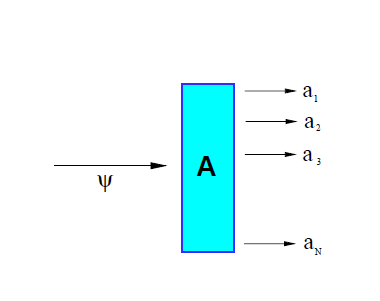
\includegraphics[width=10cm]{6_1.png}
\end{figure}

\section{تداخل}
حال به مهم‌ترین خصلت دنیای میکروسکوپی می‌رسیم. در شکل  درسمت چپ یک فیلامان حرارتی وجود دارد که بخاری از ذرات بار یونیزه را از خود متصاعد می‌کند.
 میدان‌های
الکتریکی به همراه مجموعه‌ای از یکسوکننده ها ذرات در حالت $\ket{P_{y}}$ را جدا می‌کنند. شکاف پایینی مسدود شده است.
 هر ذره
که از شکاف بالایی بگذرد درحالت $\ket{1}$ قرار می‌گیرد و سپس روی پرده در حالت ‏$\ket{y}$ که نقطه نشستن آن روی پرده را (توسط
یک آشکارساز) نشان می‌دهد، ثبت می‌شود.
 هرگاه این آزمایش را برای مدت طولانی انجام دهیم، در اثر نشستن ذرات روی
یک پرده - مثلا یک پرده فلورسانس - طرح $I_{1}$ بوجود خواهد آمد. 
$I_{1}(y)$ درواقع متناسب با تعداد ذرات نشسته شده روی نقطه $y$ است. درحقیقت داریم


\begin{equation}
	I_{1}(y) = P(y,1)P(1,P_{y})
\end{equation}

\begin{figure}[h]
	\caption{ آزمایش دو شکاف: تنها شکاف بالایی باز است و طرح $I_{1}$ روی پرده مشاهده می‌شود. }
	\centering
	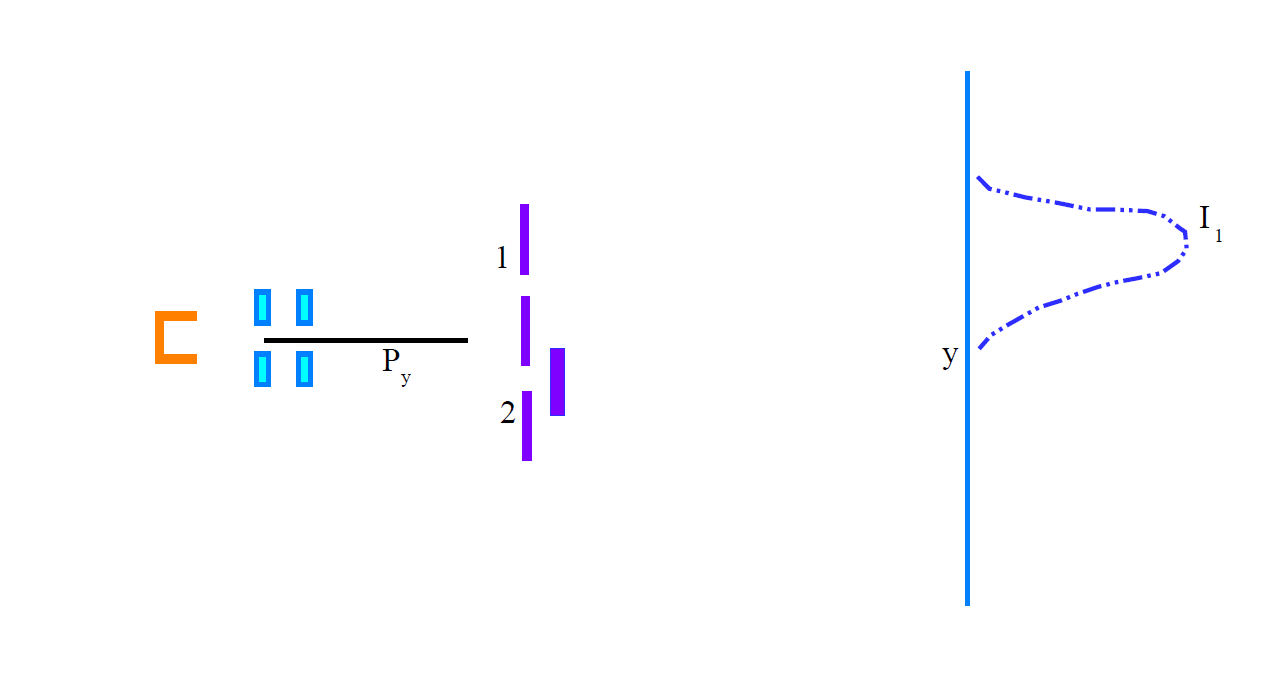
\includegraphics[width=10cm]{6_2.png}
\end{figure}
حال آزمایش را در حالتی که تنها شکاف پایینی باز باشد تکرار می‌کنیم. به همان معنا رابطه پیشین داریم: 
\begin{equation}
	I_{2} =  P(y,2)P(2,P_{y})
\end{equation}
\begin{figure}[h]
	\caption{ آزمایش دو شکاف: تنها شکاف پایینی باز است و طرح $I_{2}$ روی پرده مشاهده می‌شود. }
	\centering
	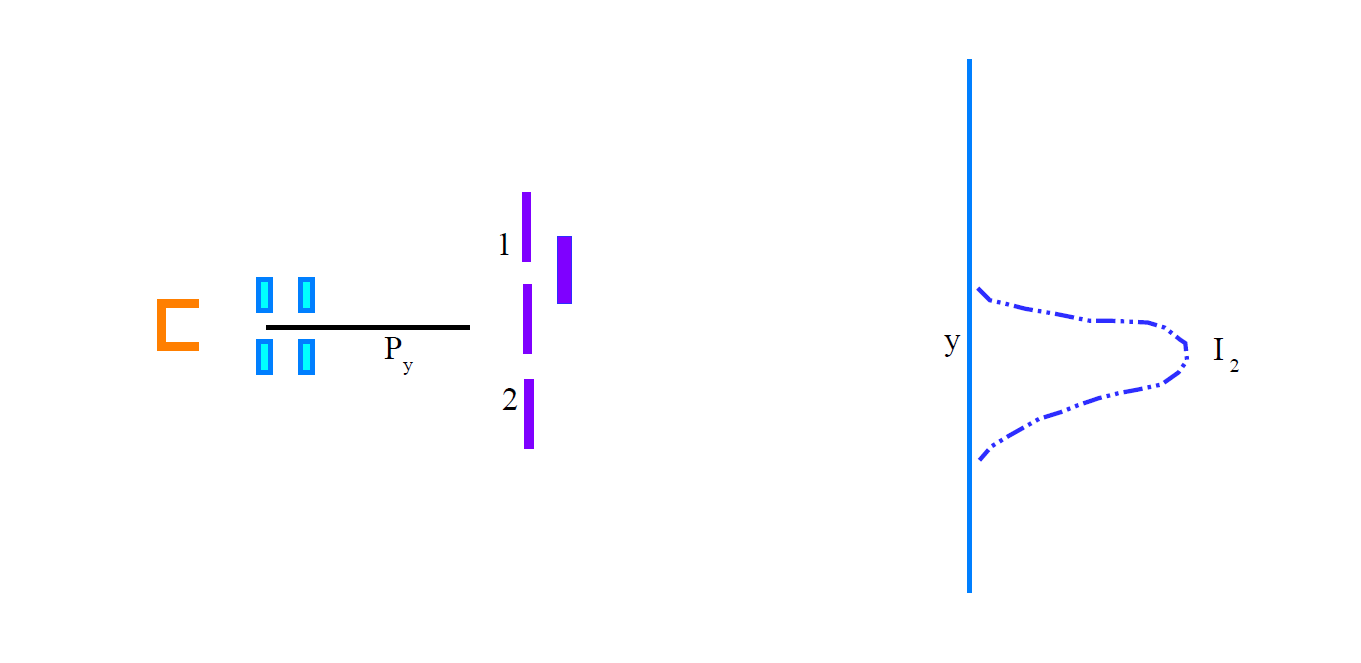
\includegraphics[width=10cm]{6_3.png}
\end{figure}
سپس آزمایش را در حالتی تکرار می‌کنیم که هر دو شکاف باز هستند. انتظار داریم این بار رابطه زیر برقرار باشد:

\begin{equation}
	I_{1 + 2} =  P(y,1)P(1,P_{y}) + P(y,2)P(2,P_{y}) = I_{1} + I_{2}
\end{equation}
و شکل \ref{fig:1} مشاهده شود.
\begin{figure}[h]
	\caption{ آزمایش دو شکاف: هر دو شکاف باز هستند و طرح $I_{1+ 2}$ روی پرده مورد انتظار است.  }
	\centering
	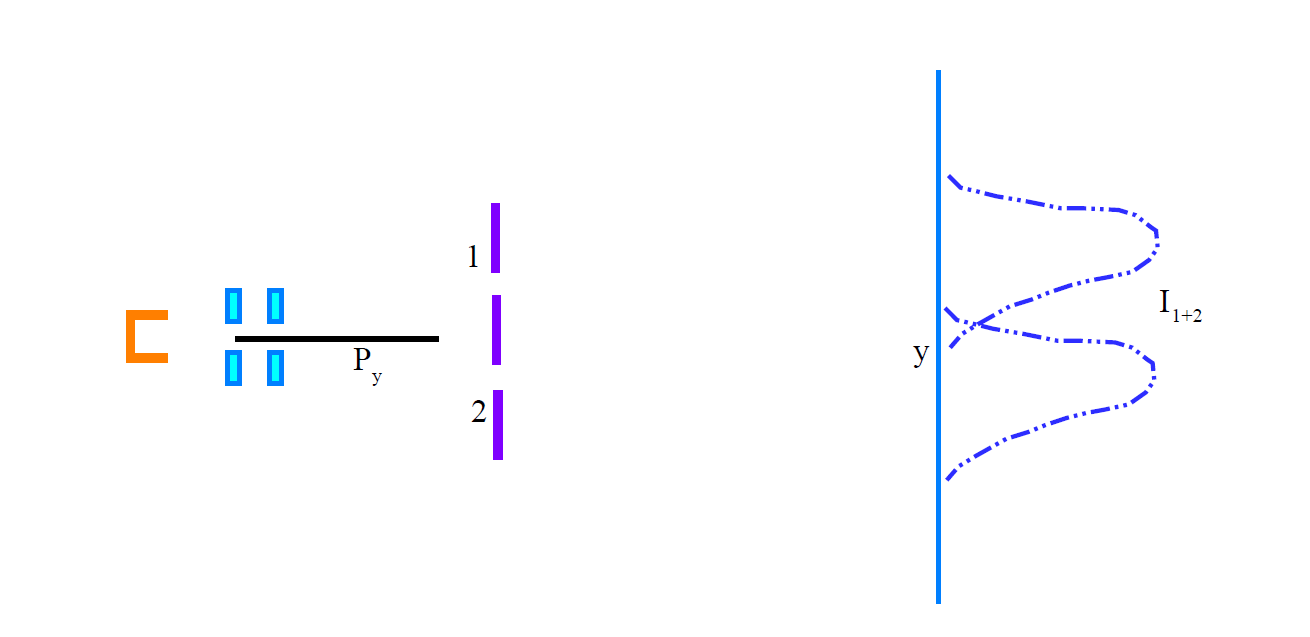
\includegraphics[width=10cm]{6_4.png}
	\label{fig:1}
\end{figure}

 


اما آنچه که در آزمایش می بینیم آن است که ذرات مطابق با طرح $I_{12}$ که یک طرح تداخلی است روی پرده می‌نشینند. (شکل \ref{fig:2})
\begin{figure}[h]
	\caption{ آزمایش دو شکاف: هر دو شکاف باز هستند و طرح $I_{1+ 2}$ روی پرده رخ می‌دهد.  }
	\centering
	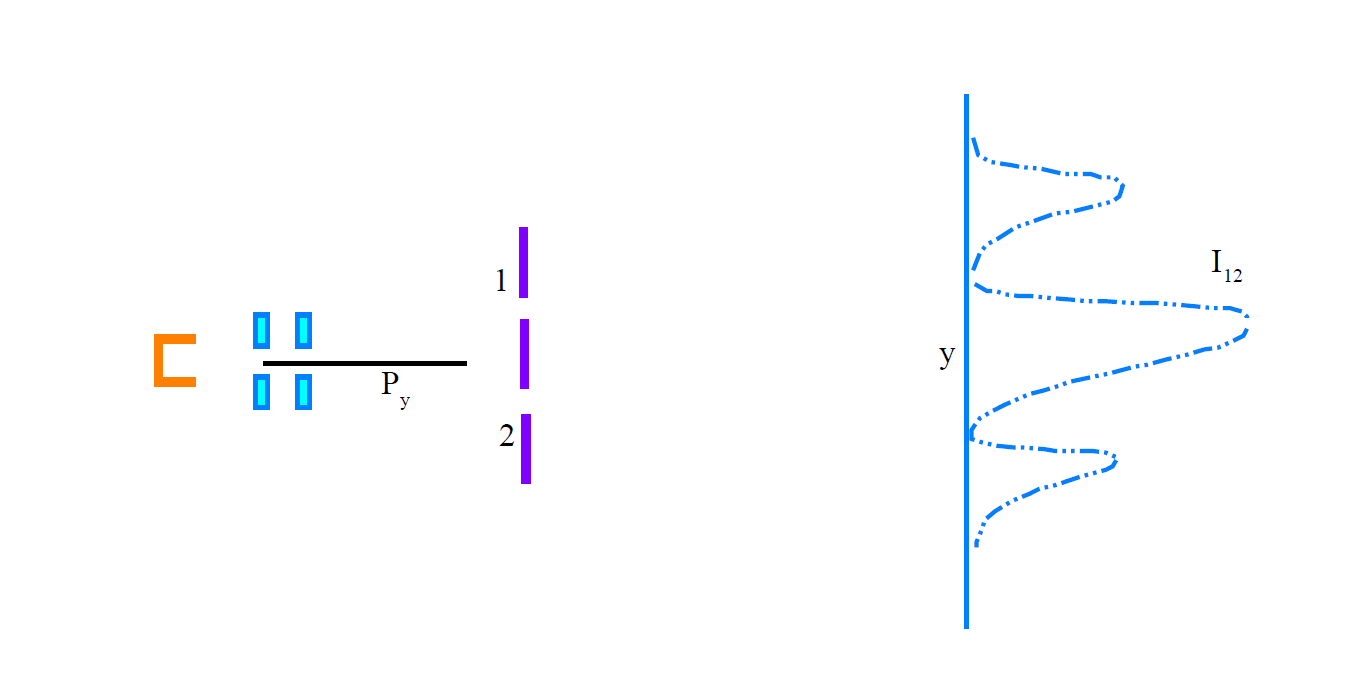
\includegraphics[width=10cm]{6_5.png}
	\label{fig:2}
\end{figure}

دراین طرح چندین نکته جالب و شگفت انگیز وجود دارد:

 

الف : در جاهایی از پرده، بازکردن هر دو شکاف با هم، باعث شده است که تعداد حتی کم‌تری ذرات نسبت به وقتی که تنها یک
شکاف بازبود به آن نقطه برسد. در جاهایی نیز مثل وسط پرده تعداد ذرات دو برابر آن مجموع تعداد ذراتی است که درصورت
باز بودن هرکدام از شکاف‌ها به تنهایی به پرده می‌رسید.

ب : برعکس درجاهای دیگری از ذرات باز کردن هر دو شکاف باعث شده است که تعداد ذراتی که به آن نقطه می‌رسد، بیشتر
از مجموع ذراتی شود که درصورتی که هر دو شکاف باز می‌بود به آن نقطه می‌رسید.

ج : شکل این طرح تداخلی با رقیق کردن چشمه ذرات بطوری که درهر آن فقط و فقط یکی از ذرات از شکاف ها عبور کند، تغییر نمی‌کند. بنابراین نمی‌توان گفت که ذرات هنگام باز بودن هر دو شکاف با یکدیگر طوری برهم‌کنش می‌کنند که اثرات بالا
دیده شود.

د : هرکدام از ذرات را روی پرده نهایی به طور کامل توسط آشکارساز ثبت می‌کنیم و آشکارساز ما ماهیت ذره‌ای آن را
به‌خوبی تایید می‌کند. بنابراین نمی‌توان گفت که ذره در این آزمایش مثل یک موجود پیوستار عمل کرده است و بخشی از آن از
یک شکاف و بخشی دیگراز یک شکاف دیگر عبور کرده است.

  
ه: ممکن است که ذره در حین عبور از دو شکاف به صورت یک پیوستار (چیزی شبیه
یک ابر) رفتار می‌کند و سپس در انتها موقع نشستن روی پرده تمامی این ابر دوباره به صورت یک ذره کوچک متمرکز می‌شود.
برای پی بردن به راز رفتار ذره می توان درست پشت شکاف ها آشکارسازهایی گذاشت تا بفهمیم که ذره درست موقع عبور از
شکاف‌ها چگونه رفتار می‌کند. متوجه می‌شویم که درآنجا هم ذره به صورت یک ابر رفتار نمی‌کند بلکه به تمامی (با تمام جرم و بار و دیگر خصوصیات خود) درآشکار ساز ثبت می‌شود. تلاش ما برای پی بردن به راز رفتار ذره باعث شده است که طرح تداخلی $I_{12}$
 از بین برود و جای خود را به طرح معمولی داده است. 
 
و :  منطق ساده به ما حکم می‌کند که هر ذره‌ای که
روی پرده می‌نشیند یا از شکاف ۱ آمده است یا از شکاف ۲. تعداد ذراتی که روی پرده نشسته‌اند برابرند با تعداد ذراتی که از
شکاف ۱ آمده اند + تعداد ذراتی که از شکاف ۲ آمده اند. اما تعداد ذراتی که از شکاف ۱ عبور کرده وروی پرده نشسته‌اند
برابراست با $I_{1}$ و تعداد ذراتی که از شکاف ۲ عبور کرده وروی پرده نشسته اند برابر است با $I_{2}$. پس حتی بدون مشاهده نزدیکی
شکاف‌ها می توانیم حکم کنیم که طرحی که سرانجام روی پرده ثبت می‌شود، می‌بایست برابر با $I_{1} + I_{2}$ باشد. درصورتی که اتم
ها مثل توپ فوتبال عمل کرده باشند استدلال بالا صحیح است. 
درمقابل ایراداتی ازاین نوع که « بالاخره الکترون یا ازاین شکاف عبور می‌کند ویا از آن شکاف و دراین صورت نمی‌بایست طرح تداخلی داشته باشیم» تنها می‌توانیم به این بسنده کنیم که بگوییم وقتی
سوال عبور الکترون از شکاف ها را به صورت عملی و تجربی بپرسیم می‌بنیم که طرح تداخلی واقعا از بین می‌رود
و ما به تناقضی برنمی‌خوریم. بنابراین می‌گوییم که وقتی الکترون را مشاهده نمی‌کنیم، نمی‌توانیم مسیری برای آن تعریف کنیم. 
 
 نخستین کار ما آن است که ببینیم آیا نظمی در طرح تداخلی شکل وجود دارد یا نه. به نظر می‌رسد که طرح $I_{12}$، یک طرح ناشی از تداخل امواج باشد. 
 بنابراین، برای پیداکردن نظمی که درجستجوی آن هستیم به تجربیات خود درمورد
امواج بازمی‌گردیم . اگر $I_{1}$ را مربع یک عدد مختلط $\phi_{1}$ موسوم به دامنه احتمال و $I_{2}$ را نیز مربع یک عدد مختلط $\phi_{2}$ بگیریم
چه بسا که $I_{12}$ مربع $\phi_{1} + \phi_{2}$ باشد، چنان که درمورد امواج چنین است:

 
\begin{equation}
	I_{1} := |\phi_{1}|^{2} \quad I_{2} := |\phi_{2}|^{2} \quad I_{12} =: |\phi_{12}|^{2}
\end{equation}
به طوری که 
\begin{equation}
	\phi_{12} = \phi_{1} + \phi_{2}
\end{equation}
و در معادله موج زیر، جملات سوم و چهارم که به جملات تداخلی موسوم هستند می‌توانند رفتار موجی ذرات را توجیه کنند:
 \begin{equation}
 	I_{12} = I_{1} + I_{2} + \phi_{1}\phi^{*}_{2} + \phi_{2}\phi^{*}_{1}
 \end{equation}
 
 ولی باید توضیح دهیم این اعداد مختلط چه هستند. فرایند تغییر حالت در این وضعیت، نباید به حالاتی که یک الکترون در میانه را طی می‌کند توجهی کند، پس متغیر $\phi_{12}$ دامنه احتمالی است که یک حالت اولیه را به یک حالت نهایی می‌برد:
  \begin{equation}
  	\phi_{12} = \braket{y}{P_{y}}
  \end{equation}
    \begin{equation}
  	\phi_{1} = \braket{y}{1}\braket{1}{P_{y}}
  \end{equation}
    \begin{equation}
  	\phi_{2} = \braket{y}{2}\braket{2}{P_{y}}
  \end{equation}
  توجه کنید که از نمادگذاری فوق منظوری از ضرب داخلی نداریم. در نتیجه:
   \begin{equation}
   		\braket{y}{P_{y}} = \braket{y}{1}\braket{1}{P_{y}} + \braket{y}{2}\braket{2}{P_{y}}
   \end{equation}
    این رابطه، اصل رابطه‌ای است که ساختمان نظری مکانیک کوانتومی بر اساس آن بیان می‌شود.
    \begin{equation}
    	\braket{c_{k}}{a_{i}} = \sum_{j} \braket{c_{k}}{b_{j}}\braket{b_{j}}{a_{i}}
    \end{equation}
    پس برای شکل مشخص است که می‌توانیم با آزمایش‌های مکرر، مقدار احتمال‌های زیر را حساب کنیم و داخل یک بردار به شکل زیر نشان دهیم:
    \begin{equation}
    	\ket{\Psi}_{A} = \begin{pmatrix}
    	\braket{a_{1}}{\Psi} \\ \\
    	\braket{a_{2}}{\Psi} \\ \\
    	\vdots \\ \\
    	\braket{a_{N}}{\Psi} \\ \\
    	\end{pmatrix}
    \end{equation}
    شاخص $A$ برای یادآوری آن است که اعداد داخل این بردار از اندازه‌گیری‌های $A$ به دست آمده است. 
    
   با توجه به قانون برابری احتمال 
   \begin{equation}
   P(a,b) = P(b,a) \longleftrightarrow \braket{a}{b} = \braket{b}{a}^{*}
   \end{equation}
   پس طبق رابطی کلی زیر 
   \begin{equation}
   	\braket{b_{j}}{\Psi} = \sum_{i} \braket{b_{j}}{a_{i}}\braket{a_{i}}{\Psi}
   \end{equation}
   می‌توان شاخص‌های اندازه‌گیری را حذف کرد و اطمینان دهیم که حالت ذره توسط بردار $\Psi$ توصیف شده است. با توجه به این که مقادیر بردار اندازه‌گیری احتمال هستند، ضرب‌کردن همه مقادیر در یک فاز، احتمالات را در یک شاخص اندازه‌گیری عوض نخواهد کرد. 
   
   \section{معادله شرودینگر}
   \begin{equation}
   	i\hbar \frac{\partial \psi}{\partial t} = H \psi
   \end{equation}
   معادله شرودینگر\footnote{Schrodinger Equation } نقش قوانین نیوتن در فیزیک کوانتوم را دارد. برای فهمیدن این معادله با فرمول بندی همیلتونی مکانیک کلاسیک\footnote{Hamiltonian Mechanics} شروع می‌کنیم. 
   \subsection{مکانیک همیلتونی}
   ذره‌ای با جرم $m$ را در نظر بگیرید که در یک فضای یک بعدی در حرکت است. مکان این ذره را با $q$ و تکانه\footnote{momentum} آن را با $p$ نمایش می‌دهیم و فرض می‌کنیم که ذره در پتانسیل $V = V (q, t)$ قرار دارد. در این صورت انرژی کل ذره برابر است با
   \begin{equation}
   	H = T + V
   \end{equation}
  که $T = \frac{p^{2}}{2m}$ انرژی جنبشی آن است. دو معادله زیر را در نظر بگیرید.
  \begin{equation}
  \begin{cases}
  \dot{q} = \frac{\partial H}{\partial p} & \\
  \dot{p} = - \frac{\partial H}{\partial q} & 
  \end{cases}
  \end{equation}
از آنجا که $V$ مستقل از $p$ است، داریم
\begin{equation}
	\frac{\partial H}{\partial p} = \frac{\partial T}{\partial p} = \frac{p}{m}
\end{equation}
و لذا معادله اول چیزی جز تعریف تکانه $p = m\dot{q}$ نیست. به طور مشابه از آنجا که $T$ مستقل از $q$ است از معادله دوم به دست می‌آوریم
\begin{equation}
	\dot{p} = - \frac{\partial V}{\partial q}.
\end{equation}
در نتیجه از ترکیب این دو داریم
 \begin{equation}
 	m\ddot{q} = - \frac{\partial V}{\partial q}
 \end{equation}
 که همان قانون دوم نیوتن است. در واقع معادله شرودینگر، فرمول بندی معادلی با $F = ma$ است که به آن فرمول بندی همیلتونی گفته می‌شود و کل مکانیک کلاسیک را می‌توان براساس آن پایه ریزی کرد.  
  \section{اصول مکانیک کوانتومی}
  \subsection{اصل اول - فضای حالات}
 به هر سیستم فیزیکی یک فضای هیلبرت متناظر است. حالت  سیستم (در هر لحظه از زمان)
با یک بردار ناصفر در فضای هیلبرت مشخص می‌شود. دو بردار که ضریبی از یکدیگر باشند یک حالت
فیزیکی را بیان می‌کنند. بنابراین حالت سیستم را می‌توان با یک بردار به طول یک (بردار واحد) مشخص
کرد.

فضای هیلبرت فضای برداری است که دارای ضرب داخلی باشد و نسبت به نرمی که ضرب داخلی آن القاء می‌کند، کامل باشد. توجه کنید که فضاهای ضرب داخلی با بعد متناهی همواره کامل هستند.

\begin{example}
کیوبیت یک سیستم کوانتومی است که فضای هیلبرت $H$ متناضر با آن دوبعدی باشد. اگر پایه تعامد یکه $\{\ket{0},\ket{1}\}$ را برای این فضا در نظر بگیریم، آن‌گاه داریم:
\begin{equation}
	\forall \ket{\Psi} \in H, \quad \ket{\Psi} = a\ket{0} + b\ket{1}, \quad a,b \in \mathbb{C}
\end{equation}   
\begin{equation}
	\| \ket{\Psi} \| = 1 \Rightarrow |a|^{2} + |b|^{2} = 1
\end{equation}   
بردار یکه $\frac{1}{\sqrt{2}}\ket{0} + \frac{1}{\sqrt{2}}\ket{1}$ مثالی از یک حالت است که یک کیوبیت می‌تواند داشته باشد. از آنجا که این بردار ضریبی از بردار یکه $-\frac{1}{\sqrt{2}}\ket{0} - \frac{1}{\sqrt{2}}\ket{1}$ است، این دو بردار یک حالت سیستم را نشان می‌دهند. تفاوت این دو بردار یکه ضریب کلی با نرم یک است و لذا به عنوان حالات کوانتومی، یکسان هستند. توجه کنید که این دو، با حالت $\frac{1}{\sqrt{2}}\ket{0} - \frac{1}{\sqrt{2}}\ket{1}$ متفاوت هستند چون ضریبی از یکدیگر نیستند.
\end{example}

 یک سیستم فیزیکی که بعد فضای هیلبرت متناظر آن $d$ باشد، $dim(H) = d$ یک کیودیت\footnote{Qudit} نامیده می‌شود. فضای برداری متناظر با یک کیودیت با پایه متعامد یکه زیر نمایش داده می‌شود:
  \begin{equation}
  \{ \ket{0}, \ket{1}, ... , \ket{d-1} \}
  \end{equation}
  
  \subsection{اصل دوم - تحول زمانی}
  تحول زمانی یک سیستم بسته با یک عملگر یکانی که روی فضای هیلبرت عمل می‌کند، بیان می‌شود. یعنی اگر حالت سیستم در زمان $t_{0}$، $\ket{\Psi}$ باشد و در زمان $t_{1}$، $\ket{\Psi^{'}}$ باشد، آنگاه $U \mathcal{H} \to \mathcal{H}$  یکانی وجود دارد که $U\ket{\Psi} = \ket{\Psi^{'}}$. $U$ تنها وابسته به زمان است. 
  
  این اصل در واقع فرمول بندی دیگری از اصل شرودینگر است. این معادله تحول زمانی یک سیستم کوانتومی را به صورت زیر بیان می‌کند: 
  \begin{equation}
  	i\hbar\frac{d}{dt}\ket{\Psi (t)} = H\ket{\Psi (t)}
  \end{equation}
  که در آن $H: \mathcal{H} \to \mathcal{H}$ یک عملگر هرمیتی است. اگر $H$ مستقل از زمان باشد،حل معادله دیفرانسیل فوق به صورت زیر است: 
  \begin{equation}
  	\ket{\Psi (t)} = \exp{-\frac{it}{\hbar}H}\ket{\Psi (0)}
  \end{equation}
  حال اگر قرار دهیم 
 \begin{equation}
 	U = \exp{-\frac{it}{\hbar}H}
 \end{equation}
 آنگاه معادله زمان اولیه برقرار می‌شود. می‌توان نشان داد $U$ یکانی است و این شرایط برای حالتی که $H$ مستقل از زمان هم نیست برقرار است. 
 
\begin{example}
  تحول زمانی یک کیوبیت با ماتریس‌های یکانی $2 \times 2$ مانند ماتریس‌های یکانی و هرمیتی زیر که آن‌ها را ماتریس پاولی\footnote{Pauli Matrices} می‌نامیم، بیان می‌شود: 
 \begin{equation}
 	X = \begin{pmatrix}
 		0 & 1 \\ \\
 		1 & 0 
 	\end{pmatrix}
 \end{equation}
 \begin{equation}
 	Z = \begin{pmatrix}
 		1 & 0 \\ \\
 		0 & -1 
 	\end{pmatrix}
 \end{equation}
 این عملگرها به صورت زیر عمل می‌کنند: 
 \begin{equation}
 	X(a\ket{0} + b\ket{1}) = a\ket{1} + b\ket{0}
 \end{equation}
  \begin{equation}
 	Z(a\ket{0} + b\ket{1}) = a\ket{0} - b\ket{1}
 \end{equation}
 \end{example}

 یک مثال دیگر، عملگر یکانی هادامارد\footnote{Hadamard Matrix} است: 
 \begin{equation}
 	H = \frac{1}{\sqrt{2}}\begin{pmatrix}
 		1 & 1 \\ \\
 		1 & -1 
 	\end{pmatrix}
 \end{equation}
 توجه کنید که $H$ هرمیتی هم است و داریم $H^{\dagger}XH = Z$ که نتیجه می‌دهد ویژه‌مقادیر $X$ و $Z$ یکسان است. ویژه‌بردارهای $Z$ به علت آن‌ که در پایه استاندارد قطری است برابر با $\{\ket{1}, \ket{0} \}$ است و ویژه‌بردارهای $X$ برابرند با 
 \begin{equation}
 	\{ \ket{+} := \frac{1}{2}(\ket{0} +\ket{1}), \ket{-} := \frac{1}{2}(\ket{0} - \ket{1})
 \end{equation}
 و خواهیم داشت $H\ket{0} = \ket{+}$ و $H\ket{1} = \ket{-}$.
 
  \subsection{اصل سوم - اندازه‌گیری}
اندازه گیری بر روی یک سیستم با فضای هیلبرت $\mathcal{H}$ با مجموعه‌ای به صورت 
\begin{equation}
	\{ M_{i}: M_{i}: \mathcal{H} \to \mathcal{H}, i \in S \}
\end{equation}
 مشخص می شود که :
 \begin{equation}
 	\sum_{i \in S} M_{i}^{\dagger}M_{i} = I 
 \end{equation}
 در این صورت به $M_{i}$ها عملگرهای اندازه‌گیری می‌گویند. با انجام این اندازه‌گیری، اگر حالت سیستم $\ket{\Psi} \in \mathcal{H}$ باشد، حاصل اندازه‌گیری با احتمال $p(i) = \ev{M_{i}^{\dagger}M_{i}{\Psi}}$ برابر می‌شود. اگر هم حاصل اندازه گیری $i$ باشد، حالت سیستم به 
 \begin{equation}
 	\ket{\Psi^{'}} = \frac{M_{i}\ket{\Psi}}{\sqrt{p(i)}}
\end{equation}  
تغییر\footnote{collapse} می‌کند.

\begin{example}
اندازه‌گیری یک کیوبیت، اگر $M_{i} = \dyad{v_{i}{v_i}}$ باشد، آنگاه می‌توان نشان داد که $\{ M_{0}, M_{1},...,M_{d-1}\}$ یک اندازه‌گیری است. 
پس اگر حالت سیستم به صورت $\ket{\Psi} = \sum_{i} a_{i}\ket{v_{i}}$ باشد، آنگاه
\begin{equation}
	p(i) = \ev{M_{i}^{\dagger}M_{i}}{\Psi} = |a_{i}|^{2}
\end{equation}
\end{example}

\begin{example}
اندازه‌گیری تصویری: عملگرهای تصویر را در نظر بگیرید. می‌توان نشان داد که $\{ P_{i}: i \in S \}$ یک اندازه‌گیری است. به چنین اندازه‌گیری تصویری می‌گویند. توجه کنید که در اندازه‌گیری تصویری، برای هر $i \ne j$ می‌توان نشان داد $P_{i}P_{j} = 0$. در واقع اگر تصویر $P_{i}$ را با $W_{i}$ نشان دهیم، آنگاه $\mathcal{H} = \bigoplus_{i \in S} W_{i}$ افراز فضا به زیرفضاهای عمود بر هم است. 
\end{example}

\begin{example}
یک مشاهده‌پذیر\footnote{Observable} فیزیکی با یک عملگر هرمیتی روی فضای هیلبرت مشخص می‌شود: 
\begin{equation}
A: \mathcal{H} \to \mathcal{H}
\end{equation}
مثلا، عملگر همیلتونی متناظر با مشاهده‌پذیر انرژی است. از آن‌جایی که $A$ هرمیتی است، در پایه‌های متعامد یکه، قطری می‌شود. در واقع، اگر $\lambda_{i} \in \mathbb{R}$ ویژه‌مقادیر $A$ باشند و $W_{i}$‌ها زیرفضاهای تولید شده توسط ویژه‌بردارهای متناظر با $\lambda_{i}$ باشند، و $P_{i}$ را عملگر تصویر عمود بر روی این زیرفضا بگیریم، آنگاه 
\begin{equation}
	A = \sum_{i}\lambda_{i}P_{i}
\end{equation}
و از آنجا که بردارهای ویژه $A$ کل $\mathcal{H}$ را می‌پوشانند، داریم $\sum_{i} P_{i}$. پس اندازه گیری $\{P_{i}\}$ را داریم. 

اگر حالت $\ket{\Psi}$ را با $\{P_{i}\}$ اندازه‌گیری کنیم و حاصل اندازه‌گیری $i$ باشد، آنگاه می‌گوییم مقدار مشاهده‌پذیر $A$ برابر با $\lambda_{i}$  است. در این صورت، امید ریاضی این مشاهده پذیر که با $\expval{A}$ نشان داده می‌شود برابر است با
\begin{equation}
	\expval{A} = \sum_{i} \lambda_{i} p(i)  = \sum_{i} \lambda_{i} \mel{\Psi}{P_{i}}{\Psi} = \mel{\Psi}{\sum_{i} \lambda_{i} P_{i}}{\Psi} = \mel{\Psi}{A}{\Psi}
\end{equation}
\end{example}

\subsection{اصل چهارم - سیستم های ترکیبی}
فضای هیلبرت متناظر با یک سیستم فیزیکی که متشکل از $n$ سیستم کوچک‌تر است از ضرب تانسوری فضاهای کوچک‌تر بدست می‌آِید. 

به عبارت دیگر، اگر فضای هیلبرت متناظر با سیستم$i$-م $\mathcal{H}_{i}$ باشد، فضای هیلبرت متناظر با کل $n$ سیستم برابر است با 
\begin{equation}
	\mathcal{H}_{1} \otimes \mathcal{H}_{2} \otimes ... \otimes \mathcal{H}_{n}.
\end{equation} 
اگر سیستم $i$-م در حالت $\ket{\Psi_{i}} \in \mathcal{H}_{i}$ باشد، کل سیستم در حالت 
\begin{equation}
	\Psi_{1} \otimes \Psi_{2} \otimes ... \otimes \Psi_{n}.
\end{equation}
است. 

\section{درهم‌تنیدگی\footnote{Entanglement}}
دو کیوبیت  $A$ و $B$ را در نظر بگیرید. $\mathcal{H}_{A}$ و $\mathcal{H}_{B}$ فضای هیلبرت معادل هر کدام از این کیوبیت‌ها با پایه‌های $\{ \ket{0}_{A}, \ket{1}_{A}\}$ و $\{ \ket{0}_{B}, \ket{1}_{B}\}$ نمایش داده می‌شود. طبق اصل چهارم، فضای هیلبرت متناظر با سیستم ترکیبی این دو کیوبیت برابر است با 
 \begin{equation}
 	\mathcal{H}_{AB} = \mathcal{H}_{A} \otimes \mathcal{B}
 \end{equation}
 که با پایه متعامد یکه 
 \begin{equation}
 	\{ \ket{0}_{A} \otimes \ket{0}_{B}, \ket{0}_{A} \otimes \ket{1}_{B}, \ket{1}_{A} \otimes \ket{0}_{B},\ket{1}_{A} \otimes \ket{1}_{B}\}
 \end{equation}
  مشخص می‌شود که برابر است با:
    \begin{equation}
 	\{ \ket{00}_{AB}, \ket{01}_{AB}, \ket{10}_{AB},\ket{11}_{AB}\}.
 \end{equation}
 هر $\ket{\psi}_{AB} \in \mathcal{H}_{AB}$ به صورت ترکیب خطی از چهار عضو مجموعه بالاست. اگر $\ket{\psi}_{AB}$ را $\ket{\psi}_{AB} = \ket{v}_{A} \otimes \ket{w}_{B}$ نمایش داد به این حالت، حالت ضربی\footnote{Product State } و یا حالت جداپذیر\footnote{Seperable State} گفته می‌شود. اگر چنین نمایشی برای $\ket{\psi}_{AB}$ وجود نداشته باشد، به آن حالت درهم‌تنیده\footnote{Entangled State} می‌گویند. 
 \textbf{مثال: }
 \begin{equation}
 	\frac{1}{\sqrt{2}}(\ket{00} + \ket{01}) = \frac{1}{\sqrt{2}} \ket{0}_{A} \otimes (\ket{0}_{B} + \ket{1}_{B})
 \end{equation}
 یک حالت ضربی است و 
 \begin{equation}
 	\frac{1}{\sqrt{2}}(\ket{00} + \ket{11})
 \end{equation}
  یک حالت درهم‌تنیده‌است. 
  \section{اختتامیه‌ای بر عجایب مکانیک کوانتومی}
 کنترل اتم‌های منفرد و به همراه آن گسترش رایانش و اطلاعات کوانتومی منجر به پیدایش سوال‌های جدید در ساختمان نظری مکانیک کوانتومی
شده‌است. تلاش برای پاسخ‌گویی به این سوال‌ها به نوبه خود منجر به غنی شدن نظریه مکانیک کوانتومی از جهات متعدد شده است. به عنوان مثال،
چگونه می‌توان درهم‌تنیدگی دو حالت مثل 
\begin{equation}
	| \phi \rangle = \sqrt{0.9}|0,0\rangle + \sqrt{0.1}|1,1\rangle
\end{equation}
و 
\begin{equation}
	| \phi \rangle = \sqrt{0.8}|0,0\rangle + \sqrt{0.2}|1,1\rangle
\end{equation}
را با هم مقایسه کرد؟
مثل هر ویژگی دیگری در فیزیک باید بتوانیم به صورت کمی مقدار درهم‌تنیدگی این دو حالت را با هم مقایسه کنیم.

چگونه می‌توان بیشتر از دو ذره را در هم تنیده کرد؟ اکنون می‌توانیم جفت فوتون هایی را که بیش از یکصد و پنجاه کیلومتر از یکدیگر دور هستند، در‌هم‌تنیده کنیم. سوال این است که چگونه
می‌توانیم با انجام آزمایش در هرکدام از آزمایشگاه‌ها مقدار این درهم‌تنیدگی را کم و زیاد کنیم. 
چگونه می‌توانیم این کار را برای جفت فوتون‌هایی که بین زمین و ماهواره ها درهم تنیده هستند انجام دهیم؟ چگونه می توانیم اتم‌های ساکن دور از هم را درهم تنیده کنیم؟ آیا می‌توانیم شبکه‌ای از حالت های درهم تنیده بین نقاط مختلف و دور از هم درست کنیم و از آن برای مبادله اطلاعات کوانتومی و فرابرد کوانتومی استفاده کنیم؟

سوالات در مورد درهم تنیدگی نه تنها از نظر عملی مهم هستند بلکه از نظر ریاضی نیز اهمیت دارند. ما شناخت نسبتا کاملی از فضای هیلبرت
دو کیوبیت داریم. مثلا می‌دانیم که حالتی مثل
\begin{equation}
	| \phi \rangle = \sqrt{0.5}|0,0\rangle + \sqrt{0.5}|1,1\rangle
\end{equation}
بیشترین میزان درهم تنیدگی را دارد و تمام حالت های دیگر را با اعمال موضعی می توان از این حالت درست کرد. در واقع می توانیم با سنجش
درهم‌تنیدگی تمام بردارهای فضای هیلبرت، دو ذره را مرتب کنیم. ولی به محض اینکه به فضای هیلبرت سه کیوبیت می رسیم با انواع سوال‌های
جدید و بی پاسخ مواجه می‌شویم و این وضعیت ساده از بین می رود. هیچ ملاک مقایسه‌ای نداریم که بر مبنای آن بگوییم کدام یک از دو حالت
\begin{equation}
	| GHZ \rangle = \sqrt{0.5}|0,0,0\rangle + \sqrt{0.5}|1,1,1\rangle
\end{equation}
یا 
\begin{equation}
	| W \rangle = \sqrt{1/3}(|1,0,0\rangle + |0,1,0\rangle +  |0,0,1\rangle )
\end{equation}
در هم تنیدگی بیشتری دارند. این گونه مطالعات به ما کمک می‌کنند که ملاک‌های معینی برای دسته بندی حالت‌های فضای هیلبرت دو و چند
ذره‌ای ابداع کنیم و بتوانیم فضای بسیار بزرگ هیلبرت را برای یک سیستم چند ذره‌ای بر اساس این خاصیت‌ها شناسایی کنیم. سوال‌ها و کشفیات
جدید البته منحصر به در هم تنیدگی نیستند و حوزه‌های خیلی وسیعی را در بر می‌گیرند. در ادامه به یک نوع دیگر از این سوال‌ها می‌پردازیم.
\section{قضایای عدم امکان در مکانیک کوانتومی}
در سال‌های اخیر و بعد از توجه دوباره به مبانی مکانیک کوانتومی، معلوم شده است که بعضی اعمال را در دنیای میکروسکوپی هرگز نمی‌توان
انجام داد. این قضایای عدم امکان\footnote{No go theorems} اهمیت نظری و عملی بسیار زیادی دارند. به عنوان مثال قضیه عدم تکثیر\footnote{No Cloning Theorem} که یک قضیه بسیار ساده
ولی مهم و بنیادی در مکانیک کوانتومی است ، تنها در سال 1982 یعنی هشتاد سال بعد از پیدایش مکانیک کوانتومی کشف شد . در زیر، یکی
از این قضایای عدم امکان را، که همگی به تازگی کشف شده‌اند، بیان می‌کنیم.
\subsection{تکثیر حالت‌های کوانتومی}
نخست ساده ترین حالت رادر نظر می‌گیریم. حالتی که می‌خواهیم آن راتکثیر کنیم با $|\phi\rangle$ نشان می‌دهیم. حالتی را که می خواهیم یک نسخه از $|\phi\rangle$ روی آن نوشته شود را با $|b\rangle$ نشان می‌دهیم. این حالت حکم کاغذ سفید را دارد و به همین دلیل آن را حالت سفید یا حالت خالی می‌نامیم. حالت  دستگاه را نیز با $|m\rangle$ نشان می دهیم. فرض کنید که یک عمل یکانی وجود دارد که برای هرحالت ورودی کار زیر را انجام می‌دهد: 
\begin{equation}
	U(|\phi\rangle\otimes|b\rangle\otimes|m\rangle) = |\phi\rangle \otimes |\phi\rangle \otimes |m_{\phi}\rangle)
\end{equation}
دراین صورت این دستگاه حالت یک نسخه از حالت ورودی را روی حالت سفید می‌نویسد و حالت خود دستگاه نیز بسته به حالت ورودی تغییر می‌کند. درخروجی دو نسخه از حالت $|\phi\rangle$ داریم. حال دو حالت متعامد $|0\rangle$ و $|1\rangle$ را در نظر می‌گیریم. حالت‌ زیر را هم در نظر بگیرید:
\begin{equation}
	|+\rangle = \frac{1}{\sqrt{2}} (|1\rangle + |0\rangle)
\end{equation}
حال، سه حالت $|0\rangle$ و $|1\rangle$ و $|+\rangle$ را به داخل ماشین تکثیر می‌فرستیم. دقت کنید که این دوحالت لزوماً دو حالت از یک سیستم دوبعدی نیستند. دراین صورت خواهیم داشت: 
\begin{equation}
	U(|0\rangle\otimes|b\rangle\otimes|m\rangle) = |0\rangle \otimes |0\rangle \otimes |m_{0}\rangle
\end{equation}
و 
\begin{equation}
	U(|1\rangle\otimes|b\rangle\otimes|m\rangle) = |1\rangle \otimes |1\rangle \otimes |m_{1}\rangle
\end{equation}
و
\begin{equation}
	U(|+\rangle\otimes|b\rangle\otimes|m\rangle) = |+\rangle \otimes |+\rangle \otimes |m_{+}\rangle
\end{equation}
اماهرگاه تساوی سوم را بسط دهیم و ازدو رابطه اول و خطی بودن مکانیک کوانتومی استفاده کنیم به رابطه زیر می‌رسیم:
\begin{equation}
|0\rangle|0\rangle|m_{0}\rangle + |1\rangle|1\rangle|m_{1}\rangle = 
\frac{1}{\sqrt{2}}(|0\rangle|0\rangle + |0\rangle|1\rangle + 
					|1\rangle|0\rangle + |1\rangle|1\rangle)|m_{+}\rangle
\end{equation}
هرگاه طرفین این رابطه را یک‌بار در $\langle 0|\langle 0|$ و یک‌بار در $\langle 1|\langle 1|$ ضرب کنیم، با استفاده از خاصیت متعامد بودن $|0\rangle$ و $|1\rangle$ به نتیجه زیر می‌رسیم:
\begin{equation}
	|m_{+}\rangle = \sqrt{2}|m_{0}\rangle = \sqrt{2}m_{1}\rangle
\end{equation}  
با جایگذاری این رابطه در رابطه قبلی و مقایسه دوطرف می‌رسیم به
\begin{equation}
	|0\rangle|1\rangle + |1\rangle|0\rangle = 0
\end{equation}
هرگاه طرفین این رابطه را در $\langle 0|\langle 1|$ ضرب کنیم به رابطه $1 = 0$ می‌رسیم که تناقض است. 


\chapter{محاسبات و الگوریتم‌های کوانتومی}
 مطالب این فصل با اقتباس از 
 \cite{ 
 		nielsen10,
 		wolf19,
 		qis
 		}
 تهیه شده است.
  
\subsection{محدودیت‌های رایانش کلاسیک}
در کنگره ریاضیدانان در سال ١٩٠٠ دیوید هیلبرت ٢٣ مسئله مهم را بیان کرد که در واقع نقشه راهی بود برای ریاضیدانان در قرن بیستم.
 در این
میان، مسئله دهم هیلبرت جایگاه ویژه ای دارد چرا که تلاش برای حل آن توسط آلن تورینگ ریاضیدان انگلیسی منجر به ابداع نظریه رایانش
کلاسیک شد.
 نظریه‌ای که یک دهه قبل از ظهور اولین رایانه‌ها و ماشین‌های محاسبه پدید آمد و اهمیت آن در این است که خیلی پیش از ساخت
اولین کامپیوترها نشان داد که کامپیوترها چه نوع مسائلی را هرگز نخواهند توانست حل کنند.
 معادلات چندجمله‌ای با ضرایب صحیح مثل $x^{3} + y^{4} + z^{2} + w = 0$
 معادلات دیوفانتی\footnote{Diophantine} خوانده می‌شوند و مسئله دهم هیلبرت  طرح این سوال بود که آیا  الگوریتمی برای یافتن پاسخ به این سوال‌ها وجود دارد یا خیر.
برای پاسخ به این سوال بود که آلن تورینگ مفهوم ماشین تورینگ را به عنوان ماشینی انتزاعی برای محاسبه الگوریتمی ابداع کرد.
به این ترتیب وی نه تنها مبانی نظری علم رایانش را بنا نهاد بلکه نشان داد که این ماشین می‌تواند
هر نوع ماشین محاسبه دیگری را نیز شبیه‌سازی کند. به بیان دیگر، هر نوع مسئله‌ای که بر روی هر نوع ماشین محاسبه‌ای قابل حل باشد، توسط
ماشین تورینگ نیز قابل حل است. ماحصل کار وی اثبات این بود که پاسخ سوال هیلبرت منفی است و مسئله معادلات دیوفانتی را
نمی‌توان به صورت الگوریتمی حل کرد.

در طول بیش از ٨٠ سال که از ابداع نظریه محاسبه می‌گذرد، این اعتقاد عمومی تقویت شده‌است که هر ماشین محاسبه‌ای 
مستقل از این که از چه نوع سازوکاری فیزیکی پیروی کند، توسط ماشین تورینگ قابل شبیه‌سازی است. این نظریه یا تز که به نام تز چرچ -تورینگ شناخته می‌شود در واقع محدوده قوانین فیزیک را به نظریه محاسبه پیوند می‌دهد.

ماشین تورینگ البته یک مدل نظری محاسبه است . در عمل، مدل‌های گوناگونی می‌توانند محاسبه و رایانش را انجام دهند. رایج‌ترین مدل محاسبه مدل مداری است که در آن داده‌ها در رشته‌ای از بیت‌های کلاسیک $0$ و $1$ ذخیره می‌شوند و مدارهای منطقی کلاسیکی که از گیت‌های کلاسیک ساخته شده‌اند این داده‌ها را پردازش می‌کنند. این مدارهای منطقی می‌توانند توابع قابل محاسبه را با ترکیبی از گیت‌های منطقی $AND$ و $NOT$ و $OR$ محاسبه کند. یک بیت کلاسیک می‌تواند تنها در یکی از دو حالت $0$ و $1$ قرار بگیرد. حال آنکه بیت کوانتومی یا کیوبیت\footnote{Qubit} می تواند در ترکیبی از این دو حالت نیز قرار گیرد. یک حافظه کوانتومی شامل $n$ کیوبیت می‌تواند در ترکیبی خطی از $2^{n}$ حالت مختلف قرار بگیرد. به عنوان مثال، فرض کنید که بتوانیم از اسپین یک هسته به عنوان یک کیوبیت استفاده کنیم و بتوانیم یک کامپیوتر کوانتومی
بسازیم که تنها 1000 تا اسپین را به عنوان کیوبیت استفاده می‌کند. در این صورت یک حالت کلی از این ١٠٠٠ اسپین حالتی است که در یک فضای بسیار بسیار بزرگ $2^{1000}$ قرار دارد. حالت این کامپیوتر در هر زمان ترکیبی خطی از این تعداد حالت محاسباتی است. این ویژگی که از آن به خاصیت توازی کوانتومی\footnote{Quantum Parallelism} یاد می‌شود کامپیوتر کوانتومی را قادر می‌کند که همزمان یک تابع را برای تعداد نمایی از متغیرها محاسبه کند. 
این
قابلیت کامپیوترهای کوانتومی، آنها را قادر می‌کند که توانایی حل مسائلی را داشته باشند که حل آن‌ها برای کامپیوترهای کلاسیک زمان بسیار زیادی خواهد
برد. مشهورترین این مسائل، مسئله تجزیه یک عدد به عامل‌های اول آن است.
امروزه، می‌دانیم که با بهترین الگوریتم‌های کلاسیک، اگر بخواهیم
اعداد ۵٠٠ رقمی را با قوی‌ترین کامپیوترهای موجود حل کنیم، به زمانی از مرتبه میلیون‌ها سال نیاز داریم. اما نشان داده شده که الگوریتم‌های کوانتومی که روی کامپیوترهای کوانتومی پیاده سازی می شوند، می توانند این مسئله را در زمان خیلی کوتاه‌تری حل کنند.

\section{مبادله کوانتومی اطلاعات}
برهم‌نهی حالت‌ها اگرچه یکی از ویژگی‌های سیستم‌های کوانتومی است ولی ویژگی‌ای نیست که تنها مختص سیستم‌های کوانتومی باشد. مثلا
نور و امواج الکترومغناطیسی نیز از این ویژگی برخوردارند. یک باریکه نور می‌تواند دارای قطبش خطی در راستای افقی یا عمودی و یا ترکیبی
از هر دو راستا باشد. بنابراین باریکه نور کلاسیک از خود خاصیت برهم‌نهی نشان می‌دهد. اما آنچه که واقعا ویژگی منحصر بفرد و یکتای
مکانیک کوانتومی است، خصلت ناموضعی\footnote{Non-locality} آن است. این خصلت ارتباط نزدیکی با درهم تنیدگی\footnote{Entanglement} دارد و نشان می‌دهد که اندازه‌گیری یک
ذره در یک نقطه می‌تواند خصلت‌های بالقوه‌ای را که در یک ذره در دوردست وجود دارد، به طور آنی تغییر دهد و آن‌ها را به فعلیت درآورد، بدون
این‌که هیچ‌گونه ارتباط علی با آن ذره داشته باشد. اندازه‌گیری شما از میان تمام حالت‌های احتمالی‌ای که یک ذره در کیلومترها آن طرف‌تر می‌توانست اختیار کند، یکی را به
صورت قطعی انتخاب می‌کند، بدون اینکه نور و یا هیچ علامت دیگری فرصت کرده باشد که در بین این دو اندازه گیری این فاصله را طی کرده
باشد. امروزه، با آزمایش‌های دقیق اپتیکی می‌توانیم فوتون هایی را تولید کنیم که در فاصله‌های بیش از ١۵٠ کیلومتر از یکدیگر درهم‌تنیده باشند.  بر خلاف چهره تناقض‌گونه این خاصیت، که گمان می‌رفت ناقض نسبیت خاص است، عمیق‌ترین و رازآلودترین ویژگی کوانتومی است. ویژگی‌ای که به کرات در ادامه این گزارش از آن استفاده خواهیم کرد. تا قبل از سال‌های آغازین دهه آخر قرن بیستم، فیزیکدانان توجه خود را معطوف به تلاش برای درک این خصلت کرده بودند. 

تنها پس از شصت سال که
توجه عموم فیزیکدانان معطوف به بررسی جنبه های معنایی درهم تنیدگی شده بود نخستین کاربردهای مهم و تکان دهنده درهم تنیدگی پدیدار
شدند. نخست در سال ١٩٩١ معلوم شد که از حالت های درهم‌تنیده می توان برای توزیع کوانتومی کلید\footnote{Quantum Key Distribution} برای رمزنگاری\footnote{Quantum Cryptography} استفاده کرد و
سپس در 1995 معلوم شد که می‌توان حالت کوانتومی ذرات را با سرعت نور از یک نقطه به نقطه دیگر انتقال داد. اگر قبول کنیم که یک شئ
چیزی نیست جز حالت کوانتومی آن، این پدیده که به آن فرابرد کوانتومی\footnote{Quantum Teleportation} می‌گوییم، در واقع نخستین نمونه از جابجایی اشیا با سرعت نور
خواهد بود. اینکه یک شی ماکروسکوپی را نیز بتوان با استفاده از این پدیده با سرعت نور جابجا کرد در حال حاضر به طور کامل دور از دسترس
علم و فناوری است. اخیرا نشان داده شده است که با طراحی یک آزمایش دو شکاف می‌توان طرح‌های تداخلی را حتی برای مولکول‌هایی به بزرگی فولرین یا $C^{60}$ مشاهده کرد. اما این برهم‌نهی و خصلت کوانتومی تا به کجا ادامه پیدا می‌کند؟ آیا یک پروتئین ، یا سلول، یک گربه یا یک انسان نیز می تواند در یک برهم‌نهی از حالت‌هایش قرار بگیرد؟ در حال حاضر می‌دانیم که یک انسان می‌تواند در مکان $A$ یا در مکان $B$ قرار بگیرد، ولی در یک برهم‌نهی از این دو حالت نه. حتی اگر در چنین حالتی قرار داده شود برهم کنش‌هایی که با محیط خود دارد بلافاصله حالت او را به یکی از دو حالت
تقلیل می دهد. این پدیده که به آن وادوسی\footnote{Decoherence} می‌گوییم، برای اشیای ماکروسکوپی با سرعت سرسام آوری رخ می‌دهد به نحوی که این اشیا هرگز
در چنین حالت‌هایی دیده نمی‌شوند و حال آنکه اشیای میکروسکوپی مثل الکترون و اتم می‌توانند درچنین حالت‌هایی قرار بگیرند. به اصطلاح زمان
وادوسی برای الکترون و اتم طولانی و برای موجودات ماکروسکوپی بسیار کوتاه است. البته این وضعیت امروزین است. این که آیا می‌توان
در آینده یک شی ماکروسکوپی مثل یک گربه را آنقدر از محیط اطرافش جدا کرد و آنقدر تاثیرات محیطی را روی آن کاهش داد که زمان وادوسی‌اش طولانی شود، موضوعی است که هنوز چیزی درباره آن نمی‌دانیم. حتی ممکن است که این وادوسی تنها ناشی از برهم‌کنش با محیط نباشد
بلکه ناشی از خصلت ماکروسکوپی خود شی و تعداد زیاد اتم‌های موجود در آن باشد که در این صورت انجام فرابرد کوانتومی برای این گونه اشیا به کلی منتفی خواهد بود. به هرحال این موضوع که دقیقا مرز دنیای ماکروسکوپی و میکروسکوپی یا به اصطلاح مرز بین دنیای کلاسیک
و کوانتومی کجاست، سوالی است که پاسخ آن تا به امروز مشخص نیست. ممکن است که هیچ مرز مشخصی بین این دو دنیا وجود نداشته باشد که در این
صورت با پیشرفت تکنولوژی ممکن است صدها سال بعد بتوان یک گربه را نیز در برهم‌نهی از دو حالت یا چند حالت‌اش نگاه داشت و ممکن
است که یک ثابت بنیادی جدید در طبیعت کشف شود که مرز بین این دو دنیا را مشخص کند.
\section{شبیه‌سازی کوانتومی}
یک دستگاه ساده کلاسیکی مثل منظومه شمسی را در نظر بگیرید. این دستگاه دارای $N$ ذره (اعم از خورشید، سیارات، قمرها و سیارک‌ها و ستارگان دنباله‌دار) است که همگی تحت نیروی گرانش حرکت می‌کنند. هر کدام از این ذرات با سه مختصه برای مکان و سه مختصه برای سرعت
یا تکانه مشخص می‌شوند. هم چنین از انجا که سیارات را نمی‌توان به صورت نقاط بدون بعد در نظر گرفت می‌توان برای هر کدام سه مختصه که نشان‌دهنده وضعیت دورانی آن‌ها باشد نیز در نظر گرفت. بنابراین تعداد کل متغیرهایی که برای توصیف این سیستم به کار می‌رود برابر است با $9N$. 
 
 می‌توان مقدار هرکدام از این متغیرها را در یک آرایه از کامپیوتر ذخیره کرد و سپس مطابق با قوانین نیوتن مقدار هر کدام از این متغیرها را لحظه به
لحظه پیدا کرد. به این ترتیب می‌توان رفتار این دستگاه کلاسیکی را در یک کامپیوتر شبیه‌سازی کرد و توسط این برنامه شبیه‌سازی می‌توان کسوف
ها و خسوف‌ها و برخوردهای احتمالی و ده‌ها پدیده دیگر را در منظومه شمسی پیش بینی کرد. نکته مهم در اینجا این است که تعداد متغیرهایی
که می‌بایست در حافظه کامپیوتر ذخیره کرد نسبت به تعداد اشیای موجود در منظومه شمسی به صورت خطی رشد می‌کند. هرگاه که تعداد ذرات را
به عنوان مثال دو برابر کنیم کافی است که مقدار حافظه کامپیوتر را دو برابر کنیم. این خصلت بسیاری از سیستم های کلاسیک است که با افزایش
تعداد ذرات ، تعداد متغیرهای توصیف کننده وضعیت این سیستم‌ها به صورت چندجمله‌ای رشد می‌کند. به همین ترتیب است که می‌توان نه تنها منظومه شمسی بلکه رفتار خوشه های ستاره‌ای، کهکشان‌ها و خوشه‌های کهکشانی و یا رفتار دستگاه‌های فناوری را در کامپیوترها شبیه سازی کرد. 


حال به یک سیستم کوانتومی ساده توجه می‌کنیم. ماده بس‌ذره‌ای که از همه درجات آزادی اتم‌های آن صرف نظر کرده و فقط اسپین اتم‌های آن را در نظر گرفته‌ایم. اگر $N$ تا اتم داشته باشیم و هر اتم یک ذره اسپین $1/2$ باشد، تعداد حالت‌های اسپینی این اتم‌ها برابر است با $2^{N}$.
 بنابراین، هر حالت بردار سیستم یک بردار $2^{N}$ مولفه‌ای است و اگر بخواهیم دینامیک چنین سیستم ساده‌ای را با کامپیوترهای کلاسیک شبیه‌سازی کنیم، می‌بایست $2^{N}$  عدد را که نشان دهنده این بردار حالت در هر لحظه است در حافظه کامپیوتر ذخیره کنیم. بدلیل نمایی بودن این بعد احتیاج به یک حافظه خیلی خیلی بزرگ داریم. کافی است که برای سادگی یک سیستم 1000 اتمی را تصور کنید. حالت کوانتومی چنین سیستمی، یک بردار با $2^{1000} = 10^{300}$ مولفه است . واضح است که ذخیره کردن چنین اعدادی در توان هیچ کامپیوتر کلاسیکی نیست.
 با این مثال ساده می‌بینیم که برخلاف سیستم‌های کلاسیک، سیستم‌های کوانتومی را هرگز نمی‌توان در کامپیوترهای کلاسیک شبیه سازی کرد.
 
این در حالی است که در ابعاد میکروسکوپی و در سطح بنیادین ماده تمامی سیستم‌ها رفتار کوانتومی دارند و ما برای درک رفتار ماده در مقیاس میکروسکوپی احتیاج به شبیه‌سازی رفتار ذرات و میدان‌های کوانتومی داریم. چگونه می‌توانیم از این بن‌بست راهی به بیرون بیابیم؟
نخستین بار ریچارد فاینمن راه برون رفت را نشان داد. برای شبیه‌سازی سیستم‌های کوانتومی می‌بایست از خود سیستم‌های کوانتومی استفاده کرد. به
زبان امروزی، این راه چنین است. گروهی از اتم‌ها را تصور کنید که در شرایط خاص و تحت کنترل شما قرار گرفته‌اند. تعداد این اتم‌ها از مرتبه
١٠٠٠ تا بیشتر است. این اتم‌ها می‌توانند در یک شبکه نوری\footnote{Optical Lattice} قرار گرفته باشند. یک شبکه نوری، شبکه‌ای متشکل از امواج ایستاده
است که اتم‌ها مثل تخم‌مرغ‌های درون یک شانه تخم‌مرغ در درون فرورفتگی‌های آن قرار می گیرند. می توان روی این اتم‌ها انواع گیت‌های
کوانتومی را اعمال کرد که مثل این است که بتوانیم دینامیک متناظر با هر نوع هامیلتونی را در مورد این اتم‌ها اعمال کنیم. می‌توانیم کاری کنیم که
درجات آزادی این سیستم و نوع هامیلتونی آن خیلی نزدیک به درجات آزادی و نوع هامیلتونی یک سیستم دیگر باشد که می‌خواهیم شبیه‌سازی‌اش کنیم. حتی می‌توانیم برهم‌کنش‌ها را طوری تنظیم کنیم که این سیستم دوبعدی یک سیستم سه‌بعدی را شبیه‌سازی کند.

در این صورت، حالت اولیه این مجموعه اتم‌ها را مطابق با حالت اولیه سیستم مورد نظر خود به صورت فیزیکی تهیه
می‌کنیم و اجازه می دهیم که این سیستم با هامیلتونی خاصی که برایش تدارک دیده‌ایم تحول پیدا کند. بعد از گذشت زمان دلخواه می‌توانیم هر
نوع مشاهده‌پذیری از این سیستم را اندازه گیری کنیم. این اندازه گیری را می‌توانیم بارها و بارها تکرار کنیم تا متوسط مشاهده‌پذیر را محاسبه
کنیم. به این ترتیب می‌توانیم کمیت‌های مورد نظر خود را از سیستم واقعی بدست بیاوریم. شبیه‌ساز ما به این ترتیب و به صورت واقعی یک سیستم کوانتومی دیگر را شبیه‌سازی می‌کند. این شبیه‌ساز حتی قادر است که میدان‌های کوانتومی را نیز با تقریب خوبی شبیه سازی‌کند. از نظر
فناوری دیر نخواهد بود که ما بتوانیم در شبیه‌ساز کوانتومی خود میدان‌های کوانتومی ای نظیر میدان الکترو ضعیف و یا میدان کرومودینامیک
 را شبیه سازی کنیم و بتوانیم به سوال های بنیادی در مورد ساختار ماده پاسخ گوییم.

\section{فرابرد کوانتومی}
درفرابرد کوانتومی، هدف ما آن است که بامخابره اطلاعات کلاسیک حالت کوانتومی یک شی را به نقطه‌ای دوردست انتقال دهیم. درساده ترین حالت فرض کنید که آلیس یک کیوبیت $S$  در اختیار دارد و می‌خواهد آن را به باب منتقل کند. فرض کنید کیوبیت $S$ در حالت $\ket{v}_{S} = \alpha \ket{0} + \beta\ket{1}$ قرار دارد و آلیس و باب از آن مطلع نیستند. اگر بین آلیس و باب یک کانال وجود داشت که به وسیله آن می‌توانستند کیوبیت (اطلاعات کوانتومی) انتقال دهند، مسأله انتقال $S$ ساده بود (کافی بود آلیس کیوبیت خود را در ورودی کانال قرار دهد). ولی فرض کنید که بین آنها فقط یک کانال برای انتقال اطلاعات کلاسیک (مانند تلفن معمولی) وجود دارد. سؤال این است که آیا در این صورت نیز انتقال $S$ امکان‌پذیر است یا خیر. نکته‌ای که باید به آن توجه کنیم آن است که چرا اصولا نیاز است که کانالی با خواص کوانتومی برای انتقال یک حالت یا یک کیوبیت وجود داشته باشد؟ برای انتقال کامل یک کیوبیت از طریق کانال ارتباطی کلاسیک، لازم است که مقادیر مختلط $\alpha$ و $\beta$ مخابره بشوند که برای مخابره دقیق این مقادیر نیاز به بی‌نهایت مخابره داریم، حتی تخمین آن‌ها هم مخابره زیادی از نظر تعداد بیت ارسالی می‌طلبد.  

فرض کنید که آلیس و باب هر کدام یک کیوبیت دیگر دارند که مستقل از $S$ در حالت درهم‌تنیده 
\begin{equation}
	\ket{\Phi^{+}}_{AB} = \frac{1}{\sqrt{2}} (\ket{00} + \ket{11} )
\end{equation}
آماده سازی شده‌اند. پس در کل سه کیوبیت داریم. کیوبیت‌های $A$ و $S$ در دست آلیس هستند و کیوبیت $B$ در دست باب. 

حال، پایه متعامد یکه بل\footnote{Bell basis} را برای فضای دو کیوبیت در نظر بگیرید: 
\begin{equation}
	\mathcal{B} = \{ \ket{\Phi^{+}}, \ket{\Phi^{-}}, \ket{\Psi^{+}}, \ket{\Psi^{-}} \}
\end{equation}
که در آن 
\begin{equation}
	\ket{\Phi^{\pm}} = \frac{1}{\sqrt{2}} (\ket{00} \pm \ket{11} ) \quad \ket{\Psi^{\pm}} = \frac{1}{\sqrt{2}} (\ket{01} \pm \ket{10} ).
\end{equation}
توجه کنید که داریم: 
\begin{equation}
\begin{split}
	&\ket{00} = \frac{1}{\sqrt{2}} (\ket{\Phi^{+}} + \ket{\Phi^{-}} ) \quad \ket{01} = \frac{1}{\sqrt{2}} (\ket{\Psi^{+}} + \ket{\Psi^{-}} ),\\
	&\ket{10} = \frac{1}{\sqrt{2}} (\ket{\Psi^{+}} - \ket{\Psi^{-}} ) \quad \ket{11} = \frac{1}{\sqrt{2}} (\ket{\Phi^{+}} - \ket{\Phi^{-}} ).
	\end{split}
\end{equation}

حال، سیستم ترکیبی هر سه کیوبیت در حالت $\ket{v}_{S} \otimes \ket{\Phi^{+}}$ است که اگر $SA$ را در پایه بل بنویسیم داریم: 
\begin{equation}
\begin{split}
	& \ket{v}_{S} \otimes \ket{\Phi^{+}}_{AB} = \frac{1}{\sqrt{2}}[ \alpha\ket{00}_{SA}\ket{0}_{B} + \alpha\ket{01}_{SA}\ket{1}_{B} + \alpha\ket{10}_{SA}\ket{0}_{B} + \alpha\ket{11}_{SA}\ket{1}_{B} \\
	& = \frac{1}{2} [\alpha(\ket{\Phi^{+}} + \ket{\Phi^{-}})_{SA}\ket{0}_{B} + \alpha(\ket{\Psi^{+}} + \ket{\Psi^{-}})_{SA}\ket{1}_{B} \\ 
	& + \beta(\ket{\Psi^{+}} - \ket{\Psi^{-}})_{SA}\ket{0}_{B} + \beta(\ket{\Phi^{+}} - \ket{\Phi^{-}})_{SA}\ket{1}_{B}] 
	\\ & = \frac{1}{2} [ \ket{\Phi^{+}_{SA}}(\alpha\ket{0} + \beta\ket{1})_{B} + \ket{\Phi^{-}_{SA}}(\alpha\ket{0} - \beta\ket{1})_{B} \\ 
	& + \ket{\Psi^{+}_{SA}}(\alpha\ket{0} + \beta\ket{1})_{B} + \ket{\Psi^{-}_{SA}}(\alpha\ket{0} - \beta\ket{1})_{B}
	]
	\end{split}
\end{equation}
اگر ماتریس‌های پاولی را به خاط بیاوریم:
 \begin{equation}
 	X = \begin{pmatrix} 0 & 1 \\ \\ 1 & 0 \end{pmatrix} \quad Z = \begin{pmatrix} 1 & 0 \\ \\ 0 & -1 \end{pmatrix}
 \end{equation}
  خواهیم داشت
  \begin{equation}
  \ket{v}_{S} \otimes \ket{\Phi^{+}}_{AB} = \frac{1}{2} [\ket{\Phi^{+}}_{SA}\ket{v}_{B} + \ket{\Phi^{-}}_{SA}\otimes Z\ket{v}_{B} +  \ket{\Psi^{+}}_{SA}\otimes X\ket{v}_{B} \ket{\Psi^{-}}_{SA}\otimes XZ\ket{v}_{B}]
  \end{equation}
  فرض کنیم آلیس دو کیوبیتی که در اختیار دارد، یعنی $SA$ را در پایه بل اندازه‌گیری کند. در این صورت عملگرهای اندازه‌گیری آلیس برابرند با
  \begin{equation}
  	M_{1} = \dyad{\Phi^{+}}{\Phi^{+}}, \quad M_{2} = \dyad{\Phi^{-}}{\Phi^{-}} \\
  	M_{3} = \dyad{\Psi^{+}}{\Psi^{+}}, \quad M_{4} = \dyad{\Psi^{-}}{\Psi^{-}} \\
  \end{equation}
  
  اگر برای مثال حاصل اندازه‌گیری آلیس $M_{1}$ باشد، با توجه به محاسبات فوق سیستم به حالت زیر تغییر می‌کند:
  \begin{equation}
  	(M_{1,SA} \otimes I_{B}) \ket{v}_{S} \otimes \ket{\Phi^{+}}_{AB} = (\dyad{\Phi^{+}}{\Phi^{+}} \otimes I_{B}) \ket{v}_{S} \otimes \ket{\Phi^{+}}_{AB} = \frac{1}{2}\ket{\Phi^{+}}_{SA}\ket{v}_{B}
  \end{equation}
  یعنی کیوبیت باب به حالت $\ket{v}$ تغییر پیدا می‌کند.در واقع بسته به حاصل اندازه‌گیری آلیس، تغییر کیوبیت باب به صورت زیر خواهد بود:
  \begin{equation}
  	\begin{split}
  	&  M_{1} \Rightarrow \ket{V}, \quad M_{2} \Rightarrow Z\ket{V},\\
  	& M_{3} \Rightarrow X\ket{V}, \quad M_{4} \Rightarrow XZ\ket{V}.
  	\end{split}
  \end{equation}
  
  حال فرض کنید که آلیس بعد از انجام اندازه‌گیری، نتیجه را با استفاده از 2 بیت کلاسیک فوق برای باب ارسال کند. در این صورت باب با توجه تناظر فوق می‌تواند وارون ماتریس پائولی مناسب را بر کیوبیت خود اعمال و حالت $\ket{v}$ به دست می‌آورد. 
  
  توجه کنید که در این پروتکل، اندازه‌گیری آلیس چهار حالت دارد. پس آلیس 2 بیت اطلاعات کلاسیک برای باب می‌فرستد. همچنین حالت $\ket{\Phi^{+}}_{AB}$ که آلیس و باب از قبل با هم قسمت کرده بودند، یک واحد درهم‌تنیدگی یا ای-بیت\footnote{Entanglement bit or ebit}  نامیده می‌شود. به طور خلاصه
  \begin{equation}
  	1 \, ebit + 2 \, bit \rightarrow 1 \, qubit
\end{equation}   

\section{کدگذاری چگال}
مساله کدگذاری چگال\footnote{Superdense Coding} دقیقا برعکس فرابرد است. یعنی، با در اختیار داشتن یک کانال کوانتومی، چگونه اطلاعات کلاسیک مخابره کنیم. در این آلیس و باب دو کیوبیت را مانند حالت قبل در حالت درهم‌تنیده 
 \begin{equation}
 \ket{\Phi^{+}}_{AB} = \frac{1}{\sqrt{2}} (\ket{00} + \ket{11} )
 \end{equation}
 تقسیم کرده‌اند. آلیس 2 بیت کلاسیک دارد که می‌خواهد به باب منتقل کند. ولی کانال بین آنها یک کانال کوانتومی است.   در اینجا نشان می‌دهیم که این کار با انتقال تنها 1 کیوبیت امکان‌پذیر است. در واقع
    \begin{equation}
  	1 ebit + 1 qubit \rightarrow 2 bit
\end{equation} 
نمادگذاری زیر را در نظر بگیرید: 
\begin{equation}
	\begin{split}
		& \sigma_{00} = I, \quad \sigma_{01} = X, \\
		& \sigma_{10} = Z, \quad \sigma_{11} = ZX.
	\end{split}
\end{equation}
توجه کنید که این چهار عملگر یکانی هستند. پس آلیس می‌تواند هر یک از آن‌ها را بر کیوبیت خود $A$ اثر دهد. داریم
\begin{equation}
	\begin{split}
		& \sigma_{00}^{A} \otimes I^{B}\ket{\Phi^{+}} = \ket{\Phi^{+}}, \quad \sigma_{01}^{A} \otimes I^{B}\ket{\Phi^{+}} = \ket{\Phi^{-}}, \\
		& \sigma_{10}^{A} \otimes I^{B}\ket{\Phi^{+}} = \ket{\Psi^{+}}, \quad \sigma_{11}^{A} \otimes I^{B}\ket{\Phi^{+}} = \ket{\Psi^{-}}, \\
	\end{split}
\end{equation}
پس نتیجه یکی از بردارهای پایه بل می‌شود و از آنجا که این حالت‌ها بر هم عمود هستند، اگر آلیس بعد از اثر دادن عملگر $\sigma_{ij}$ کیوبیت خود را برای باب بفرستد، باب می‌تواند به طور دقیق تشخیص دهد که این دو کیوبیت در چه حالتی هستند و از آنجا می‌فهمد که آلیس کدام $\sigma_{ij}$ را اثر داده است. 

به طور دقیق‌تر، فرض کنید دو بیت آلیس $i,j \in {0,1}$ پروتکل این طور شروع می‌شود که آلیس $\sigma_{ij}$ را روی کیوبیت $A$  اعمال می‌کند و بعد این کیوبیت را از طریق کانال کوانتومی برای باب می‌فرستد. حال، باب  دو کیوبیت $A$ و  $B$ را در اختیار دارد و آنها را در پایه بل اندازه می‌گیرد (پس عملگرهای متناظر این اندازه‌گیری از رابطه به دست می‌آیند).  از آنجا که چهار حالت $\sigma_{ij} \otimes I\ket{\Phi^{+}}$ بر هم عمودند، این اندازه‌گیری آن‌ها را از هم بدون خطا تشخیص می‌دهد. پس باب از روی حاصل اندازه‌گیری، می‌تواند $i,j$ را بیابد. 

\section{الگوریتم‌های کوانتومی}
\subsection{کیوبیت}
 مفهوم مرکزی در کامپیوتر کوانتومی بیت کوانتومی یا کیوبیت است. یک حافظه کوانتومی $n$-کیوبیتی\footnote{n-qubit Quantum Register} عبارت است از مجموعه‌ای متشکل از $n$ کیوبیت. فضای هیلبرت این حافظه عبارت است از: 
  \begin{equation}
  	(\mathcal{C}^{2})^{\otimes n} = \{ \sum_{s_{0},s_{1},...,s_{n-1} \in {0,1}} \alpha_{s_{0},s_{1},...,s_{n-1}} \ket{s_{0},s_{1},...,s_{n-1}} \}
  \end{equation}
  و بعدِ آن برابر است با $2^{n}$. دقت کنید که این حافظه می بایست چنان باشد که تمام بردارهای فضای هیلبرت آن قابل دسترسی باشند. بنابراین اگر دو کیوبیت را تنها کنارهم بگذاریم به این معنی نیست که یک حافظه دو کیوبیتی ساخته‌ایم. زیرا بردارهای فضای هیلبرت دو کیوبیت جداگانه به صورت زیر هستند: 
  \begin{equation}
  	\ket{\phi} \otimes \ket{\phi} = (\alpha\ket{0} + \beta\ket{1}) \otimes (\alpha^{'}\ket{0} + \beta^{'}\ket{1})
  \end{equation}
  
  یعنی به صورت ضرب تنسوری دو بردار از فضاهای هرکدام از کیوبیت‌ها نوشته می‌شوند و حال آنکه در فضای هیلبرت دِو  کیوبیت یعنی 
  $(\mathcal{C}^{2})^{\otimes 2}$بردارهایی وجود دارند که به صورت فوق قابل نوشتن نیستند، مثل بردار درهم‌تنیده  $\ket{\Phi^{+}}$. برای آنکه یک بردار کلی به صورت 
   \begin{equation}
   a\ket{00} + b\ket{01} + c\ket{10} + d\ket{11}
\end{equation}    
  به صورت حاصل ضرب تانسوری دو بردار نوشته شود، می‌بایست شرط $ad - bc = 0$ برقرار شود. بنابراین بردارهایی که به صورت ضرب تنسوری هستند، مجموعه‌ای با اندازه صفر را در فضای هیلبرت دو کیوبیت تشکیل می‌دهند.
  \subsection{توازی کوانتومی}
  اولین تفاوت مهم کامپیوتر کوانتومی با کامپیوتر کلاسیک این است که یک حافظه کوانتومی می‌تواند در آن واحد در تمام حالت های بالقوه خود قرار بگیرد. این خصلت ناشی از برهم‌نهی حالت‌های کوانتومی است و اصطلاحاً توازی کوانتومی  خوانده می‌شود. هرگاه هر حالت $\ket{s_{0},s_{1},...,s_{n-1}}$ را برای کد کردن عددِ دودویی $s = (s_{0},s_{1},...,s_{n-1})$ به کار ببریم، حالتی مثل 
  \begin{equation}
  	\ket{\phi} = \sum_{s = 0}^{2^{n} - 1} \phi_{s}\ket{s}, 
\end{equation}   
حالت کلی یک حافظه $n$ کیوبیتی است. بنابراین هرگاه حافظه را در حالت $\ket{\phi}$ با ضرایب ناصفر قرار دهیم، مثل این است که همزمان آن را در تمام حالت‌های $\ket{s}$  قرار داده‌ایم. البته واضح است که هرگاه حافظه را در پایه محاسباتی اندازه‌گیری کنیم، تنها یکی از مقادیر $s$ با احتمال $| \phi_{s} |^{2}$ بدست خواهند آمد. بنابراین توازی کوانتومی اگر چه یک خاصیت مهم حافظه است ولی این خاصیت را می‌بایست با ظرافت مورد بهره برداری قرار داد. 

\subsection{گیت کوانتومی}
 اگر اطلاعات را در کیوبیت‌ها ذخیره کنیم، به ناچار پردازش اطلاعات می‌بایست
یا با عملگرهای یکانی که تحول‌ها یا اندازه‌گیری‌ها را نشان می‌دهند انجام بگیرند. معمولا اصطلاح گیت کوانتومی برای یک عملگر یکانی به‌ کار برده می‌شود. گیت کوانتومی هرگاه روی یک کیوبیت اثر کند آن را گیت تک کیوبیتی و هرگاه روی $n$تا کیوبیت اثر کند، گیت $n$ کیوبیتی خوانده می‌شود.  گیت‌های مهم همان عملگرهای یکانی مهم مانند ماتریس‌های پاولی و عملگر هادامارد هستند. نکته مهم برای گیت‌های کوانتومی در مقابل گیت‌های کلاسیک، برگشت‌پذیر بودن‌ آن‌هاست. 

\subsection{روند یک الگوریتم کوانتومی}
 الگوریتم کوانتومی در ساده ترین شکل آن به مجموعه‌ای از گیت های کوانتومی متوالی گفته می‌شود که روی یک حالت معین اولیه اثر می‌کنند و چنان تنظیم شده‌اند که حالت نهایی چنان باشد که پس از اندازه‌گیری‌های سنجیده‌ای روی آن جواب یک مسئله معین را با احتمال بسیار خوب در بر داشته باشد. 
 در ادامه چند الگوریتم مطرح کوانتومی را خواهیم دید. 
 
 \section{الگوریتم دوچ-جوزا}
 الگوریتم دوچ-جوزا\footnote{Deutsch–Jozsa} که در سال 1982 مطرح شد به حل مسأله زیر می‌پردازد. 
 
 ورودی: تابع $F: \{0,1\}^{n} \to \{0,1\}$ 
 
شرط: یا $F$ به ازای تمامی ورودی‌ها $0$ می‌دهد و یا دقیقاً به ازای نصف ورودی‌ها صفر و به ازای نصف دیگر یک است. 

  خروجی: $F$ کدام یک از دو حالت گفته شده است؟
  
  یک الگوریتم احتمالاتی کلاسیک برای حل این مسأله این است که به ازای یک ورودی دلخواه خروجی تابع را چک
کنیم. اگر یک بود حتماً تابع در حالت دوم است و اگر صفر بود، یا در حالت اول و یا در حالت دوم است که انتخاب
تصادفی یکی از این دو حالت منجر به یک الگوریتم احتمالاتی می‌شود. حال اگر به دنبال یک الگوریتم کلاسیک باشیم که بتواند به صورت قطعی پاسخ درست دهد، باید حداقل $2^{n-1} + 1$ تا از ورودی‌ها را چک کنیم. در اینجا نشان می‌دهیم  که الگوریتمی کوانتومی وجود دارد که با فقط یک بار سوال پرسیدن کوانتومی\footnote{Quantum Query} از تابع، می‌تواند به جواب قطعی برسد.
 
  \subsection{سوال پرسیدن کوانتومی}

قبل از پرداختن به الگوریتم کوانتومی توجه کنید که ابتدا باید سوال پرسیدن کوانتومی از تابع $F$ را مدل کنیم. به طور کلاسیک ما، به سادگی فرض می‌کنیم که با ورودی $x$ می‌توان خروجی $F(x)$ را بدست آورد. به طور کوانتومی ممکن این عمل را به صورت  $\ket{x} \to \ket{F(x)}$ مدل کنیم، ولی توجه کنید که سوال پرسیدن در دنیای  کوانتومی باید یکانی باشد. حال آنکه $\ket{x} \to \ket{F(x)}$ یکانی نیست چون بعد فضای ورودی و خروجی یکسان نیست. حتی اگر عملگر 
$\ket{x} \to \ket{F(x)}\ket{\underbrace{000...0}^{n-1}}$  در نظر بگیریم، باز هم یکانی نیست چون ضرب داخلی را حفظ نمی‌کند.

 سؤال پرسیدن کوانتومی از یک تابع معمولاً به یکی از دو صورت زیر مدل می‌شود. 
 \begin{equation}
 	T_{F}\ket{x} = (-1)^{F(x)}\ket{x}
 \end{equation}
  و یا 
  \begin{equation}
  	O_{F}\ket{x}\ket{y} = \ket{x}\ket{F(x)\oplus y}
  \end{equation}
  در $T_{F(x)}$ با توجه به پاسخ تابع، فاز حالت را عوض می‌کنیم و در مدل $O_{F(x)}$ با استفاده از تغییر حالت $\ket{y}$ مقدار $F(x)$ برای ما روشن می‌شود. توجه شود که هردوی این عملگرها یکانی هستند و برای 
  $\ket{\psi} = \sum_{x}\alpha_{x}\ket{x}$ داریم:
  \begin{equation}
  	T_{F(x)}\ket{\psi} = \sum_{x}\alpha_{x}(-1)^{F(x)}\ket{x}
  \end{equation}
  و 
  \begin{equation}
  	O_{F(x)}\ket{\psi}\ket{0} = \sum_{x}\alpha_{x}\ket{x}\ket{F(x)}.
  \end{equation}
  \subsection{تبدیل فوریه روی گروه $\mathcal{Z}_{2}^{n}$}
  عملکرد گیت یک کیوبیتی هادامارد روی ورودی‌های  $\ket{0}$  و  $\ket{1}$ به صورت زیر است:
   \begin{equation}
   	\begin{split}
   		& \ket{0} \rightarrow \frac{1}{\sqrt{2}}(\ket{0} + \ket{1}) \\
   		& \ket{1} \rightarrow \frac{1}{\sqrt{2}}(\ket{0} - \ket{1}) 
   	\end{split}
   \end{equation}
  پس اگر ورودی $\ket{b_{i}}$ به صورت صفر یا یک باشد، خروجی عملگر هادامارد به صورت 
  $\frac{1}{\sqrt{2}}(\ket{0} + (-1)^{b_{i}}\ket{1})$ است. 
  حال با در نظر گرفتن ورودی 
  $\ket{x} = \ket{b_{1}}, \ket{b_{2}}, \ket{b_{3}}, ..., \ket{b_{n}}$ خروجی به صورت زیر خواهد بود: 
  \begin{equation}
  \begin{split}
  	H^{\otimes n}\ket{x} & = H\ket{b_1} \otimes H\ket{b_2} \otimes ... \otimes H\ket{b_n} \\
  	& = (\frac{1}{\sqrt{2}}(\ket{0} + (-1)^{b_{1}}\ket{1})) \otimes ... \otimes (\frac{1}{\sqrt{2}}(\ket{0} + (-1)^{b_{n}}\ket{1})) \\
  	& = \frac{1}{\sqrt{2^{n}}} \sum_{a_{1},...,a_{n} \in {0,1}} (-1)^{a_{1}b_{1}+...+a_{n}b_{n}}\ket{a_{1}...a_{n}} \\
  	& = \frac{1}{\sqrt{2^{n}}} \sum_{y\in {0,1}^{n}} (-1)^{x.y}\ket{y}
  	\end{split}
  \end{equation}
  که در آن $y=a_{1}...a_{n}$، آنگاه 
  $x.y := a_{1}b_{1} + ... + a_{n}b_{n}$.
  \subsection{الگوریتم اصلی}
  روند الگوریتم را به این صورت شروع می‌کنیم:
   \begin{enumerate}
   	\item حالت $n$ کیوبیتی $\ket{0...0}$ را در نظر بگیرید. 
   	\item برای استفاده از توازی کوانتومی، همه بردارهای $n$ کیوبیتی را در یک برهم‌نهی قرار می‌دهیم. باید عملگر هادامارد را روی همه کیوبیت‌ها اعمال کنیم. 
   	\item  سپس یک بار از مدل تابع $F$ یعنی $T_{F}$ سوال می‌پرسیم. 
   	\item سپس با اعمال دوباره $H$ تبدیل فوریه می‌گیریم. 
   	 \item در نهایت حالت به دست آمده را اندازه‌گیری می‌کنیم. 
   \end{enumerate}
   \begin{equation}
   \begin{split}
   \ket{\underbrace{0...0}_{n}} & \rightarrow^{H^{\otimes n}} \frac{1}{\sqrt{2^{n}}} \sum_{x \in {0,1}^{n}} \ket{x} \\
   & \rightarrow^{T_{F}} \frac{1}{\sqrt{2^{n}}} \sum_{x \in {0,1}^{n}} (-1)^{F(x)} \ket{x} \\
   & \rightarrow^{H^{\otimes n}} \frac{1}{2^{n}} \sum_{x \in {0,1}^{n}}  (-1)^{F(x)} \sum_{y \in {0,1}^{n}} (-1)^{x.y}\ket{y} \\
   & =  \frac{1}{2^{n}} \sum_{y \in {0,1}^{n}} (\sum_{x \in {0,1}^{n}}  (-1)^{F(x) + x.y})\ket{y}
 \end{split}
   \end{equation}
   اگر در حالت اول باشیم، یعنی تابع $F$ متحد با صفر باشد، $T_{F}$ عملگر همانی است، و از آنجا که $H^{2} = I$، حالت نهایی با حالت اولیه برابر است و اندازه‌گیری نهایی به ما حالت $\ket{\underbrace{0...0}_{n}}$ می‌‌دهد. 
   
   فرض کنید که در حالت دوم باشیم. با توجه به جمله آخر، ضریب حالت 
   $\ket{\underbrace{0...0}_{n}}$ 
   در برهم‌نهی نهایی حساب می‌کنیم. چون $x.y = 0$ است، ضریب این جمله برابر است با 
   $\sum_{x \in \{0,1\}^{n}}  (-1)^{F(x)}$. اما، می‌دانیم که خروجی تابع $F$ در نیمی از ورودی‌های $0$ و در نیمی دیگر برابر با $1$ است. در نتیجه، عبارت $\sum_{x \in \{0,1\}^{n}}  (-1)^{F(x)}$ برابر با $0$ است و کل حالت نهایی برهم‌نهی شده بر حالت
     $\ket{\underbrace{0...0}_{n}}$ عمود است و و حاصل حداقل یکی از $n$ اندازه‌گیری برابر با $1$ است. 
   
   به طور خلاصه، اگر حاصل همه اندازه‌گیری‌ها $0$ شد، در حالت اول هستیم و اگر حداقل یکی از آن‌ها $1$ شد، در حالت دوم هستیم. 
   
   \section{الگوریتم جست‌وجوی گرور}
   مدل الگوریتم قبلی، از ساختار و ماهیت تابع به ما اطلاعی نمی‌دهند و صرفا با سوال پرسیدن از مدل، مقدار تابع را در ورودی مورد نظر به ما می‌دهند. گویی این مدل یک جعبه سیاه\footnote{Black Box} است که ورودی را می‌گیرد و   خروجی را با توجه به آنچه تابع روی آن اثر می‌کند، به ما می‌دهد. به این نوع مدل کردن، مدل جعبه-سیاه یا مدل جستاری می‌گویند. قابل توجه است که پیچیدگی مسائل در این مدل بر حسب تعداد سوال‌کردن‌ها محاسبه می‌شود. 
   
   \subsection{مساله}
   ورودی:
    $f: \{0,1\}^{n} \to \{0,1\}$
شرط: دقیقاً یک 
$t \in \{0,1\}^{n}$
وجود دارد که 
$f(t) = 1$.
\\ خروجی: $t$.

تعداد ورودی‌ها برابر با 
$N = 2^{n}$
می باشد. و به طور کلاسیک نمی‌توان این مساله را با پیچیدگی بهتر از 
$O(N)$
 حل کرد. الگوریتم کوانتومی گرور\footnote{Grover} توانایی حل این مساله را با
 $O(\sqrt{N})$
 سوال را دارد.
 \section{مقدمه}
 برای حل مساله فوق، سوال کوانتومی از تابع $f$ را به صورت عملگر یکانی زیر مدل می‌کنیم:
 \begin{equation}
 	T_{f}\ket{x} = (-1)^{f(x)}\ket{x}
 \end{equation}
 تعریف کنید 
 \begin{equation}
 	\ket{s} := \frac{1}{\sqrt{N - 1}} \sum_{y \in \{0,1\}^{n}, y \ne t} \ket{y}.
 \end{equation}
در نتیجه، 
$\braket{s}{t}$
و
\begin{equation}
	\ket{\phi} = \alpha\ket{t} + \beta\ket{s} \Rightarrow T_{f}\ket{\phi} = -\alpha\ket{t} + \beta\ket{s}
\end{equation}
در واقع با توجه به شکل \ref{fig:7-1} ،اعمال $T_{f}$ متناظر با قرینه کردن نسبت به بردار $\ket{s}$ است. 
\begin{figure}[h]
	\caption{ اعمال $T_{f}$ که در واقع عمل قرینه‌کردن نسبت به $\ket{s}$ است.}
	\centering
	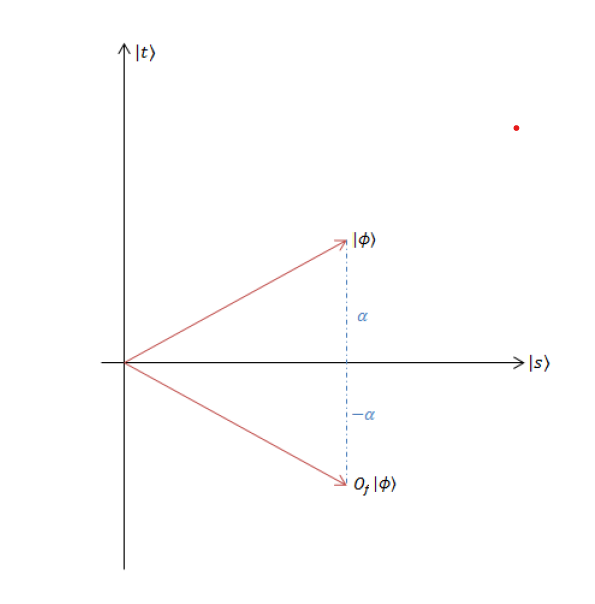
\includegraphics[width=10cm]{7_1.png}
	\label{fig:7-1}
\end{figure}
 
 بردارهای $\ket{v}$ و $\ket{w}$ را به صورت زیر تعریف کنید
 \begin{equation}
 \begin{split}
 & \ket{v} := \frac{1}{\sqrt{N}} \sum_{x \in \{0,1\}^{n}} \ket{x} \Rightarrow \ket{v} = \sqrt{\frac{N-1}{N}} \ket{s} + \frac{1}{\sqrt{N}} \ket{t} \\
 & \ket{w} :=  \frac{1}{\sqrt{N}} \ket{s} - \sqrt{\frac{N-1}{N}} \ket{t} \Rightarrow \braket{v}{w} = 0
 \end{split}
 \end{equation}
 تبدیل یکانی $U$ را در نظر بگیرید:
 \begin{equation}
 	U := H^{\otimes n}(2\dyad{0...0}{0...0} - I)H^{\otimes n} = 2H^{\otimes n}\dyad{0...0}{0...0}H^{\otimes n} - I
 \end{equation}
 می‌دانیم 
  \begin{equation}
  \begin{split}
  	& H^{\otimes n}\ket{0...0} = \frac{1}{\sqrt{2^{n}}} \sum_{x \in \{0,1\}^{n}} \ket{x} 
  	& = \frac{1}{\sqrt{N}} \sum_{x \in \{0,1\}^{n}} \ket{x} = \ket{v}
  \end{split}
  \end{equation}
  در نتیحه،
  \begin{equation}
  	U = 2\dyad{v}{v} - I
  \end{equation}
  و برای 
  $\ket{\psi} = \gamma\ket{v} + \lambda\ket{w}$ 
  داریم:
   \begin{equation}
   	U\ket{psi} = \gamma U \ket{v} + \lambda U \ket{w} = \gamma\ket{v} - \lambda\ket{w}
   \end{equation}
  نتیجه می‌شود که $U$ نسبت به $\ket{v}$ عمل قرینه انجام می‌دهد. (شکل \ref{fig:7-2})
\begin{figure}[h]
	\caption{ اعمال $U$ که در واقع عمل قرینه‌کردن نسبت به $\ket{v}$ است.}
	\centering
	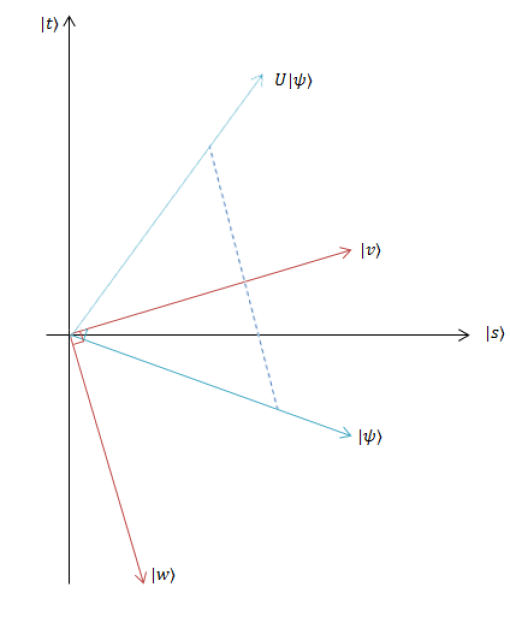
\includegraphics[width=10cm]{7_2.png}
	\label{fig:7-2}
\end{figure}

همانطور که می‌دانیم، ترکیب دو عمل قرینه، یک عمل دوران بدست می‌دهد. (شکل \ref{fig:7-3})
\begin{equation}
{f} = R_{2\theta}
\end{equation}
\begin{figure}[h]
	\caption{ $(2) = T_{f}(1), (3) = U(2)$}
	\centering
	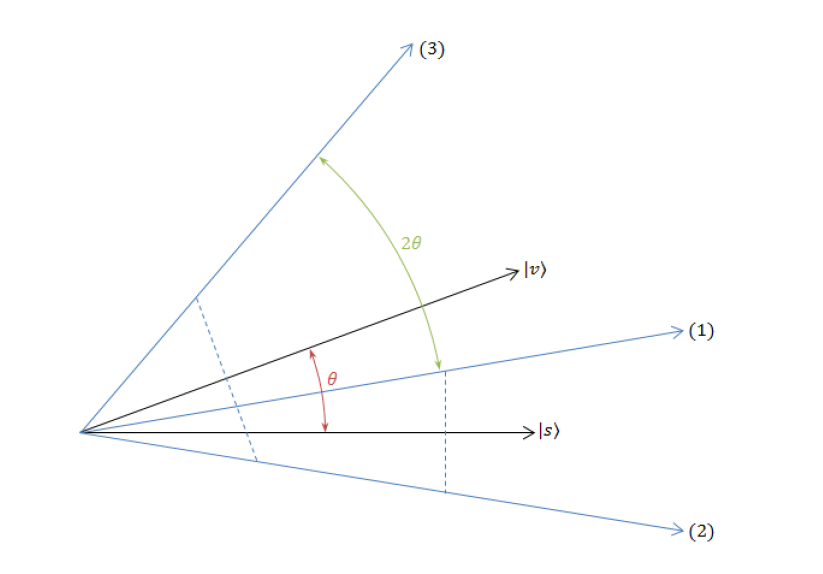
\includegraphics[width=10cm]{7_3.png}
	\label{fig:7-3}
\end{figure}
که در آن 
\begin{equation}
	cos \theta = \braket{v}{s} = \sqrt{\frac{N-1}{N}} \Rightarrow \theta \approx	\frac{1}{\sqrt{N}}
\end{equation}
\section{الگوریتم اصلی}
با $n$ کیوبیت که همگی در حالت $\ket{0}$ آماده‌سازی‌ شده‌اند شروع می‌کنیم. ابتدا، روی هر یک از $n$ کیوبیت عملگرد هامارد را اعمال می‌کنیم و بعد $R_{2 \theta}$ را $q$ بار و در آخر همه $n$ کیوبیت را اندازه‌گیری می‌کنیم: 
\begin{equation}
	\ket{0...0} \rightarrow^{H^{\otimes n}} \ket{v} \rightarrow^{(UT_{f})^{q}} \ket{\tau} \to measurement
\end{equation}
$\ket{\tau}$ یک بردار با زاویه $\theta + 2q\theta$ از $\ket{s}$ می‌باشد. اگر $q \approx \frac{\sqrt{N}}{4}\pi$ بگیریم، این زاویه تقریبا برابر با $\pi / 2$ خواهد بود. در این صورت  $\ket{\tau}$ تقریبا با $\ket{t}$ برابر است. حال با اندازه‌گیری $\tau$، حاصل اندازه‌گیری با احتمال 
\begin{equation}
	p(t) = \|\mel{t}{(UT_{f})^{q}}{v}\|^{2} = \|\braket{t}{\tau}
\end{equation}
برابر $t$ خواهد شد، و از آنجا که $\ket{t}$ و $\ket{\tau}$ به هم نزدیک است، این عدد نزدیک به $1$ است.
\chapter{پیچیدگی ارتباطی کوانتومی}
در فضای پیچیدگی ارتباطی، آیا می‌توان از مکانیک کوانتومی به نحوی بهره برد که پیچیدگی مخابره نیز کاهش یابد؟ قضیه هولف\footnote{Holevo's Theorem} نشان می‌دهد که اگر بنا باشد که فقط $n$ کیوبیت بین دو نفر جابه‌جا کنیم، امکان ندارد که بین آن دو بتوانیم چیزی فراتر از $n$ بیت کلاسیک جا‌به‌جا کنیم؛ مگر این که کیوبیت‌های دو طرف درهم‌تنیده باشند. 
\cite{holevo73}
لبته در این صورت هم فقط می‌توان دوبرابر تعداد کیوبیتی که می‌فرستیم، بیت ارسال کنیم. در یک تناقض آشکار، مسائلی وجود دارد که الگوریتم‌های توزیع شده کوانتومی، به صورت بهینه توسط سیستم کلاسیک شبیه‌سازی نمی‌شوند. در این بخش، تفاوت اطلاعات و محاسبات توزیع شده برای یک سیستم با تنظیمات کوانتومی، چه به صورت کانال کوانتومی و چه به صورت استفاده از کیوبیت‌های درهم‌تنیده را نشان ‌می‌دهیم و پروتکل‌های کوانتومی را برای چند مساله مطرح معرفی می‌‌کنیم. 
مطالب این بخش از
 \cite{wolf19, Gilles01} اقتباس شده است. 
\section{یک سوال کوانتومی}
تصور کنید که آلیس و باب مسائل پیچیدگی ارتباطی، این اجازه را داشته باشند که در یک کانال کوانتومی و با ارسال کیوبیت‌ها با هم ارتباط برقرار کنند و یا این که قبل از شروع مخابره، با هم یک حالت کوانتومی درهم‌تنیده را تقسیم کنند. 

برای مدل اول، فرض کنید که حالت بین دو طرف از سه قسمت تشکیل شده است، فضای مخفی آلیس، کانال و فضای مخفی باب. حالت شروع اولیه را برای یک تابع مانند  $f: X \times Y \to \{0,1\}$ به صورت $\ket{x}\ket{0}\ket{y}$ فرض کنید که در آن $x \in X$ ورودی آلیس است و $y \in Y$ ورودی باب و کانال در حالت اولیه $\ket{0}$ قرار دارد. حال آلیس می‌تواند محاسبات و انتقال پیام روی کانال را با استفاده از عملگرهای یکانی بر روی حالت خودش و حالت کانال انجام دهد و باب به همین ترتیب. در انتهای پروتکل، آلیس یا باب با انجام یک اندازه‌گیری، نتیجه پروتکل را اعلام می‌کند.  \cite{yao93} 

در مدل دوم، آلیس و باب تعداد نامحدودی کیوبیت درهم‌تنیده با هم به اشتراک می‌گذارند، ولی در ادامه پروتکل از یک کانال کلاسیک با قابلیت ارسال بیت معمولی استفاده می‌کنند. برای محاسبه پیچیدگی، تنها بیت‌های ارسال شده را می‌شمریم و نه تعداد ای-بیت‌ها را. پروتکلی با این سیستم را می‌توان با استفاده از پروتکل مدل اول با سربار $2$ برابر شبیه‌سازی کرد، مانند کاری که در فرابرد کوانتومی کردیم. توجه کنید که یک بیت درهم‌تنیده می‌تواند حکم یک بیت تصادفی مشترک بین آلیس و باب را داشته باشد. 
\cite{cleve97}

مدل سوم، از قدرت هر دو مدل استفاده می‌کند: آلیس و باب تعداد بی‌نهایتی کوبیت در هم تنیده در اشتراک دارند و از یک کانال کوانتومی برای انتقال اطلاعات استفاده می‌کنند. توجه کنید که این مدل هم با یک سربار با ضریب 2 معادل حالت دوم است، با استفاده از فرابرد کوانتومی. 

حال سوالی که مطرح می‌شود این است: آیا به بهبودی دست می‌یابیم؟ طبق مقدمه، قضیه هولف نشان می‌دهد اطلاعات کوانتومی مخابره شده فراتر از اطلاعات کلاسیک مخابره شده نخواهد بود مگر آنکه یک حالت درهم‌تنیده داشته باشیم. ولی مساله‌ای که با آن روبرو هستیم، مساله مخابره اطلاعات کامل نیست. در واقع آلیس یا باب علاقه‌مند به ورودی طرف دیگر نیستند، بلکه هدف این کار محاسبه یک تابع $f(x,y)$ با خروجی $1$ بیت است. مفهومی که مرز مخابره و محاسبه توزیع شده را جدا می‌کند، در مثال‌های زیر به خوبی نمایش داده شده است. 

\section{الگوریتم دوچ-جوزا: توزیع شده}\label{djd}
اولین فاصله پیچیدگی ارتباطی کوانتومی و کلاسیک، در همتای ارتباطی و توزیع شده الگوریتم پرس‌وجوی دوچ-جوزا مطرح شد.
\cite{cleve98}
در این مساله، آلیس و باب هر کدام یک رشته $n$ بیتی دارند که برای این ورودی وعده‌ای به ما داده شده است. توجه کنید که این مساله، نوع وعده‌داده‌شده\footnote{Promise Problem} از مساله برابری است. وعده مذکور به شرح زیر است:

\begin{center}
	مساله دوچ-جوزا توزیع شده: یا $x=y$ و یا $x$ و $y$ دقیقا در $n/2$ بیت‌ها با هم اختلاف دارند ($n$ سایز ورودی‌های $x$ و $y$ است).
\end{center}
حال پروتکلی را مطرح می‌کنیم که با استفاده از
 $\log(n)$ کیوبیت مساله را حل می‌کند: 
\begin{enumerate}
	\item آلیس برای باب حالت
			$\log{n}$-
				کیوبیتی 
				$\frac{1}{\sqrt{n}}\sum_{i=1}^{n}(-1)^{x_{i}}\ket{i}$ 
				را ارسال می‌کند. این حالت با استفاده از عملگر یکانی $H$ و حالت اولیه
				 $\ket{0...0}$ و عملگر یکانی $T_{f}$ به دست می‌آید. 
		
		\item  باب هم عملگر $\ket{i} \to (-1)^{y_{i}}\ket{i}$ را اعمال می‌کند و سپس عملگر هادامارد را. سپس اندازه‌گیری انجام می‌دهد.
		\item اگر خروجی اندازه‌گیری برابر با $\ket{0^{\log{n}}}$ بود، خروجی $1$ می‌دهد و در غیر این صورت خروجی $1$.
\end{enumerate}
توجه کنید که تنها
 $\log{n}$ کیوبیت مخابره شده است. همچنین، برای فهم درستی قضیه به این توجه کنید که حالتی که در نهایت باب اندازه‌گیری می‌کند، در حالت برهم‌نهی شده زیر است: 
\begin{equation}
	H^{\otimes log{n}}(\frac{1}{\sqrt{n}} \sum_{i=1}^{n} (-1)^{x_{i}+y_{i}}\ket{i}) = \frac{1}{n}  \sum_{i=1}^{n} (-1)^{x_{i}+y_{i}} +  \sum_{j \in \{0,1\}^{log{n}}} (-1)^{i.j}\ket{j}
\end{equation}
 تنها مساله‌ای که در مورد عبارت فوق باید به آن توجه کنیم آن است که ضریب پایه $\ket{0^{log{n}}}$ در هر حالت برابر با چند می‌شود. با کمی بررسی متو‌جه می‌شویم که این ضریب برابر با 
 $\frac{1}{n}\sum_{i=1}^{n}(-1)^{x_{i}+y_{i}}$ 
 که برابر با یک خواهد بود اگر و تنها اگر $x=y$. ادامه درستی مساله مانند فصل پیشین است. 
 
 این پیشرفت در مخابره درحالی است که اگر می‌خواستیم این عملیات را با مخابرات کلاسیک و قطعی انجام دهیم، پیچیدگی معادل با $O(n)$ می‌داشتیم. 
 
 
  \subsection{مساله اشتراک}

  اگر آلیس و باب هر کدام یک ورودی به اندازه $n$ بیت داشته باشند، که $x$ ورودی آلیس و $y$ ورودی باب باشد، هدف از مخابره یافتن $i$ است که $x_{i} = y_{i}$. تلاش می‌کنیم بر اساس الگوریتم جست‌وجوی گروور، یک پروتکل بهینه برای این مساله ارائه دهیم. 
  \cite{cleve98}
  لازم است ابتدا بدانیم ورودی مساله جست‌وجوی ما چیست.
  
    قرار دهید که 
  \begin{equation}
  	z_{i} = x_{i} \wedge y_{i}.
  \end{equation}
   در نتیجه مساله جست‌وجو برابر با یافتن $i$ی خواهد بود که در آن
    $z_{i} = 1$.
   ایده اصلی آن است که آلیس و باب با کمک به هم الگوریتم گروور را اجرا کنند. نکته‌ای که نیاز به همکاری در آن حس می‌شود، عملگر یکانی $T_{z}$ است. آلیس برای این که بدون آن که اطلاعاتی به صورت بیتی به باب در مورد ورودی خودش بدهد، بتواند عملگر $T_{z}$ را روی یک حالت مانند $\ket{\phi}$ اجرا کند، که 
    \begin{equation}
    	\ket{\phi} = \sum_{i=1}^{n} \alpha_{i}\ket{i}
    \end{equation}
    لازم است از یک کیوبیت کمکی استفاده کند و توجه کنید که حالت $\ket{\phi}$ یک حالت $\log{n}$ کیوبیتی است. آلیس یک کیوبیت با مقدار اولیه $0$ در کنار $\log{n}$ کیوبیت دیگر قرار می‌دهد و سپس عملگر $O_{x}$ را روی آن اجرا می‌کند:
    \begin{equation}
    \ket{\phi} \to^{ \otimes \ket{0}} \ket{\phi}\ket{0} \to^{O_{x}} T_{x}\ket{\phi}\ket{0} = \sum_{i=1}^{n} \alpha_{i}\ket{i}\ket{x_{i}}
    \end{equation}
    سپس آلیس این
     $\log{n} + 1$ کیوبیت را برای باب می‌فرستد. 
    
    باب عملگر یکانی زیر را اعمال می‌کند و سپس نتیجه را برای آلیس می‌فرستد. 
    \begin{equation}
    	\ket{i}\ket{x_{i}} \to (-1)^{x_{i}\wedge y_{i}}\ket{i}\ket{x_{i}}
    \end{equation}
    آلیس آخرین کیوبیت را برابر با $\ket{0}$ می‌گذارد (چون $x$ را دارد این عمل یکانی است). پس در نتیجه، آلیس $T_{z}\ket{\phi}$ را دارد. در نتیجه، آلیس و باب می‌توانند با $O(\log{n})$ کیوبیت مخابره، یک بار اعمال $T_{z}$ را شبیه‌سازی کنند. برای اجرای کامل الگوریتم جست‌وجو، نیاز به $\sqrt{n}$ مرحله مخابره داریم که در نهایت پیچیدگی کوانتومی 
    $O(\log{n}\sqrt{n})$ برای این مساله نشان داده می‌شود. درحالی است که این مساله حتی در حالت احتمالاتی پیچیدگی کلاسیک $O(n)$ را دارد. 
\chapter{شبیه‌سازی الگوریتم‌ها و پروتکل‌های کوانتومی}
در مورد این مساله که ذات مکانیک کوانتومی پیچیده است شکی نداریم. مساله‌ای که از آن پیچیده‌تر به نظر می‌رسد، الگوریتم‌های کوانتومی هستند. شهود بشریت با مسائلی مانند توپ و اهرم سازگارتر از مفاهیمی مانند الکترون و فوتون است و به نظر می‌رسد اتفاقاتی که در دنیای کوانتومی رخ می‌دهد چیزی شبیه جادو باشد. اما با کمی درنگ متوجه می‌شویم که همانند فیزیک کلاسیک، فیزیک کوانتومی از یک سری قائده و اصول مشخص پیروی می‌کند. اصولی که با بهره‌برداری هوشمندانه به بشریت در محاسبات، شبیه‌سازی و ... قدرتی بیش از پیش می‌دهد. برای ما، اولین قدم برای درک این قدرت محاسبات کوانتومی است. 
\section{مدار کوانتومی}
در دنیای کلاسیک، هر اطلاعاتی را می‌توان به صورت بیت‌های $0$ و $1$ نشان داد. همجنین، محاسبات را می‌توان از طریق مدارهای دیجیتالی پیش‌ برد. مداری مانند \autoref{fig:9-1} را به یاد بیاورید. 
\begin{figure}[h]
	\caption{مدار دیجیتالی ساده}
	\centering
	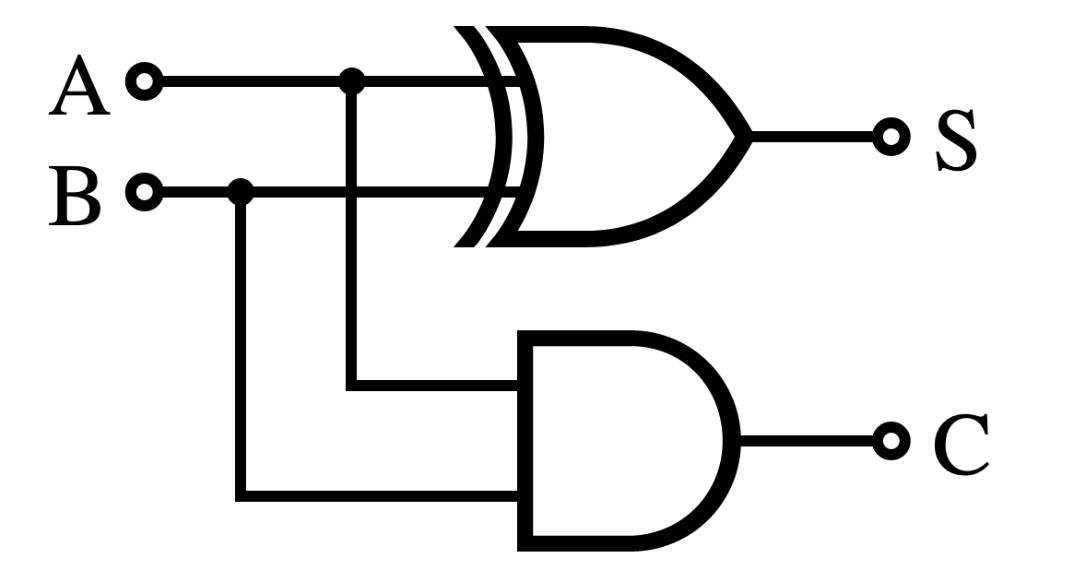
\includegraphics[width=10cm]{9_1.png}
	\label{fig:9-1}
\end{figure}
در مورد دنیای محاسبات کوانتومی نیز همین مساله صادق است. مثلا مدار کوانتومی \autoref{fig:9-2} کار مدار دیجیتالی شکل\ref{fig:9-1} را انجام می‌دهد. که همان جمع دو بیت و یا دو کیوبیت است. 
\begin{figure}[h]
	\caption{مدار کوانتومی ساده}
	\centering
	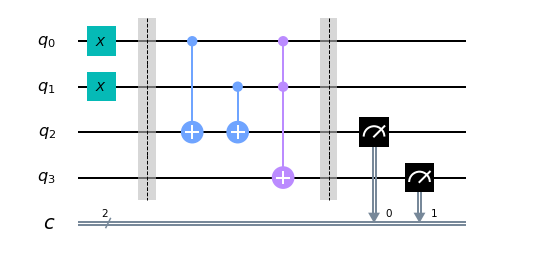
\includegraphics[width=10cm]{9_2.png}
	\label{fig:9-2}
\end{figure}
ابزاری که در ادامه برای شبیه‌سازی مفاهیم و الگوریتم‌های کوانتومی استفاده می‌کنیم کتابخانه پایتون $qisikit$
\cite{Qiskit}  محصول شرکت $IBM$ از پیشروهای علم محاسبات کوانتومی است. 
\subsection{اندازه‌گیری}
در شکل کد \ref{fig:9-3} تلاش می‌کنیم یک مدار کوانتومی ساده با اندازه اولیه $8$ کیوبیت که همه در حالت $\ket{0}$ بسازیم و سپس آن‌ها را اندازه بگیریم. 
\begin{figure}[h]
	\caption{ساخت مدار کوانتومی با $8$ کیوبیت و سپس اندازه‌گیری}
	\centering
	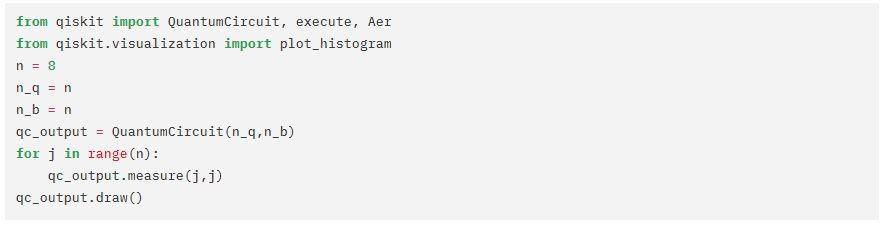
\includegraphics[width=15cm]{9_3.png}
	\label{fig:9-3}
\end{figure}
شکل مدار به صورت \ref{fig:9-4} خواهد بود. به نمادی که برای اندازه‌گیری مشخص می‌کنیم توجه کنید. 
 \begin{figure}[h]
	\caption{مدار کوانتومی اندازه‌گیری}
	\centering
	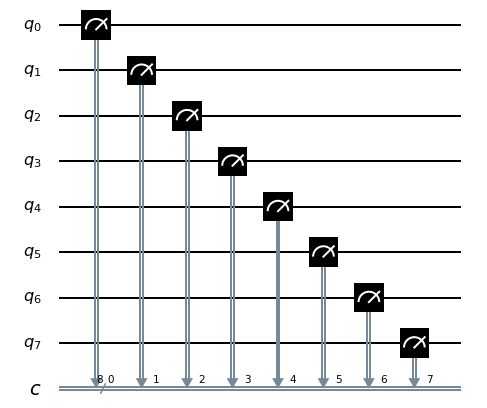
\includegraphics[width=10cm]{9_4.png}
	\label{fig:9-4}
\end{figure}
توجه کنید که کامپیوتر‌های کوانتومی و محاسبات کوانتومی شامل مقداری رفتار تصادفی هستند. به همین منظور، گاها نتایج چندین بار تکرار می‌شود تا به صورت آماری-احتمالی نتایج بررسی شود. مانند \autoref{fig:9-5}.
 \begin{figure}[h]
	\caption{بردار نتایج  بعد از چندبار اجرا}
	\centering
	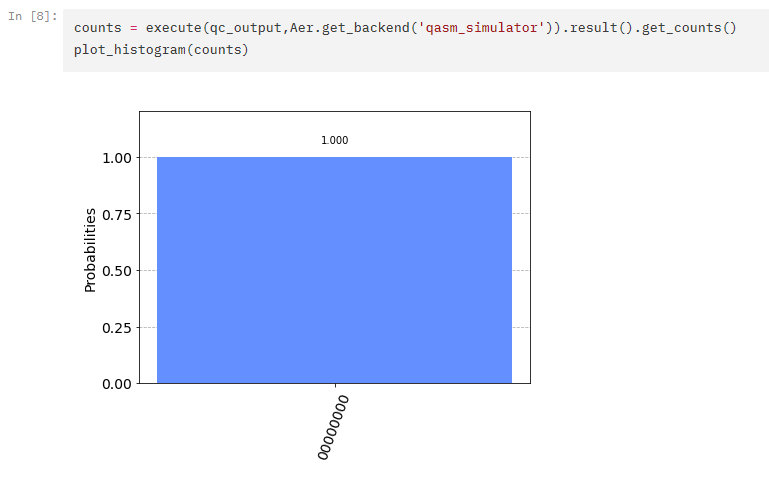
\includegraphics[width=10cm]{9_5.png}
	\label{fig:9-5}
\end{figure}
همچنین خوب است بدانیم که چون این ماشین‌های کلاسیک هستند که عملکرد ماشین کوانتومی را شبیه‌سازی می‌کنند، توانایی بیشتر از $30$ کیوبیت محاسبه را ندارند. 
\subsection{مدار جمع‌کننده}
برای طراحی مدارهای بیشتر، لازم است که با گیت‌های بیشتری آشنا شویم. به یاد داریم که گفته بودیم هر گیت کوانتومی یک عملگر یکانی است. پس عملگرهای یکانی مانند 
\begin{equation}
	  X = \begin{pmatrix} 0 & 1 \\ \\ 1 & 0 \end{pmatrix} 
\end{equation}
\begin{equation}
	  Z = \begin{pmatrix} 0 & 1 \\ \\ 1 & 0 \end{pmatrix} 
	\end{equation}
\begin{equation}
	  H =\frac{1}{\sqrt{2}} \begin{pmatrix} 1 & 1 \\ \\ 1 & -1 \end{pmatrix}  \\
\end{equation}
\begin{equation}
	 CX = \begin{pmatrix} 1 & 0 & 0 & 0 \\ \\ 0 & 1 & 0 & 0 \\ \\ 0 & 0 & 0 & 1 \\ \\ 0 & 0 & 1 & 0 \end{pmatrix}
\end{equation}
همه گیت‌های منطقی کوانتومی برگشت‌پذیر هستند. توجه کنید که عملگر دو کیوبیتی $CX$ یا نات-کنترل‌شده\footnote{Controlled-Not} عملگری است که برای هر دو کیوبیت ورودی، اگر کیوبیت اولیه برابر با $1$ باشد، خروجی دوم را $NOT$ ورودی دوم قرار می‌دهد و بالعکس. همچنین خروجی اول با ورودی اول برابر است. به  \autoref{fig:9-6} توجه کنید. ِ
\begin{figure}[h]
	\caption{گیت $CX$}
	\centering
	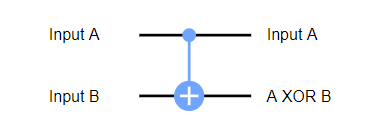
\includegraphics[width=10cm]{9_6.png}
	\label{fig:9-6}
\end{figure}
همانطور که می‌بینید، این عملگر همان $XOR$ است، اما برگشت‌پذیر هم هست‌! نکته‌ای که در دنیای دیجیتال نداریم. 

حال لازم است که یک گیت $AND$ هم داشته باشیم که برگشت‌پذیر هم باشد. گیت کوانتومی معادلی آن، گیت $Toffoli$ است  که روی فضای $3$ کیوبیت اعمال می‌شود. 
\begin{equation}
	CCX = \begin{pmatrix}
	1 & 0 & 0 & 0 & 0 & 0 & 0 & 0 \\ \\
	0 & 1 & 0 & 0 & 0 & 0 & 0 & 0 \\ \\
	0 & 0 & 1 & 0 & 0 & 0 & 0 & 0 \\ \\
	0 & 0 & 0 & 1 & 0 & 0 & 0 & 0 \\ \\
	0 & 0 & 0 & 0 & 1 & 0 & 0 & 0 \\ \\
	0 & 0 & 0 & 0 & 0 & 1 & 0 & 0 \\ \\
	0 & 0 & 0 & 0 & 0 & 0 & 0 & 1 \\ \\
	0 & 0 & 0 & 0 & 0 & 0 & 1 & 0
	\end{pmatrix}
\end{equation}
این گیت، اگر دو کیوبیت ورودی اول $1$ باشند، خروجی $1$ می‌دهند. 

حال لازم است مدار را بسازیم:
\begin{enumerate}
	\item لازم است که دو بیت اول با هم $XOR$ بشوند تا بیت کم ارزش مشخص شود.
	\item  برای مشخص کردن بیت پر ارزش هم لازم است که دو کیوبیت با هم $AND$ بشوند. 
	 \item برای این‌کار‌ها، 4 کیوبیت تعریف می‌کنیم. دو ورودی، دو خروجی و دو بیت کلاسیک برای اندازه گیری.   
\end{enumerate}
کد \autoref{fig:9-7} قرار است دو کیوبیت در حالت  $\ket{1}$ و $\ket{1}$ را جمع کند. 
\begin{figure}[h]
	\caption{کد مدار جمع‌کننده }
	\centering
	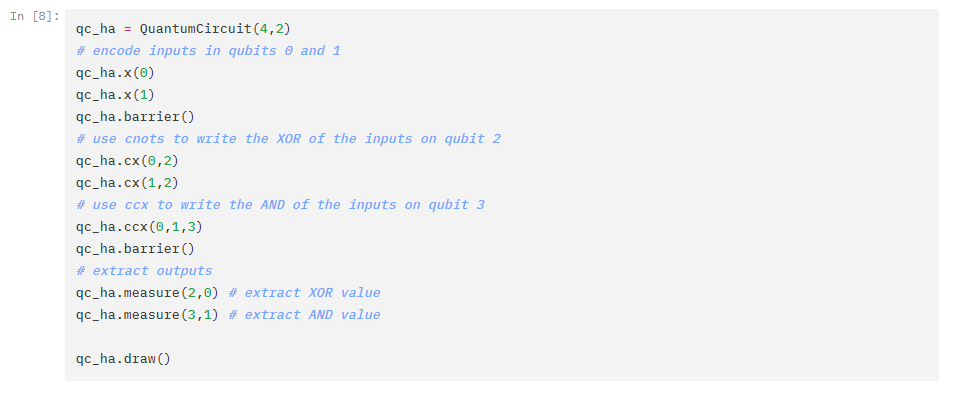
\includegraphics[width=15cm]{9_7.png}
	\label{fig:9-7}
\end{figure}
مدار نهایی در شکل \ref{fig:9-8} نشان داده شده است. مانند حالت پیشین تعدادی بار این کار را تکرار می‌کنیم تا نتیجه را ببینم. (شکل \ref{fig:9-9})
\begin{figure}[h]
	\caption{مدار جمع‌کننده}
	\centering
	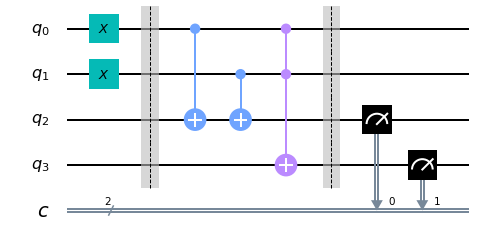
\includegraphics[width=10cm]{9_8.png}
	\label{fig:9-8}
\end{figure}
\begin{figure}[h]
	\caption{تکرار مدار}
	\centering
	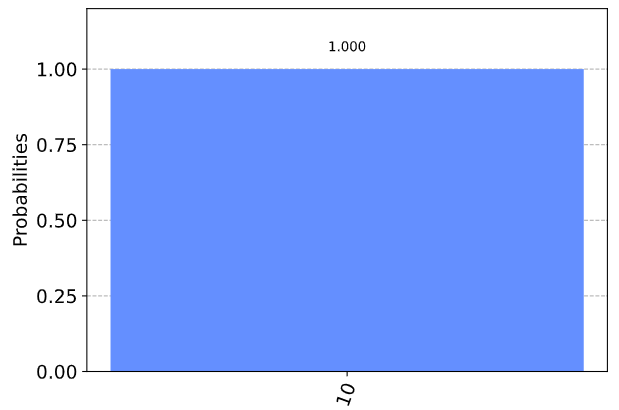
\includegraphics[width=6cm]{9_9.png}
	\label{fig:9-9}
\end{figure}
\section{فرابرد کوانتومی}
در این مرحله، یک کد ساده برای اجرای فرابرد کوانتومی اجرا می‌کنیم. مراحل کار را به یاد می‌آوریم:
\begin{enumerate}
	\item ابتدا آلیس و باب می‌بایست دو کیوبیت درهم‌تنیده در اشتراک بگذارند.
	\item آلیس عملگر هادامارد را روی کیوبیتی که می‌خواهد ارسال کند، اجرا می‌کند. 
	\item آلیس مقدار کیوبیت خود و کیوبیت ارسالی را اندازه می‌گیرد. 
	\item  مقدارهای به دست آمده را در اختیار باب می‌گذارد.
	\item باب با توجه به مقادیر به دست آمده، عملگرهای مختلف را روی کیوبیت خودش اعمال می‌کند.
\end{enumerate}
در شکل \ref{fig:9-10} کد مربوط به این کار را می‌بینید. در \autoref{fig:9-11} که مدار نهایی را نشان می‌دهد، کیوبیت اول بنا است که ارسال شود. کیوبیت دوم و سوم در‌هم‌تنیده شده‌اند و کیوبیت دوم در اختیار آلیس و کیوبیت سوم در اختیار باب است. در نهایت، نتیجه اندازه‌گیری آلیس بر روی دو ثبات کلاسیک می‌نشیند که در اختیار باب است و با توجه به نتیجه آن‌ها، عملگرهای $X$ و $Z$ را روی کیوبیت خود اجرا می‌کند. 
\begin{figure}[h]
	\caption{کد مدار فرابرد کوانتومی}
	\centering
	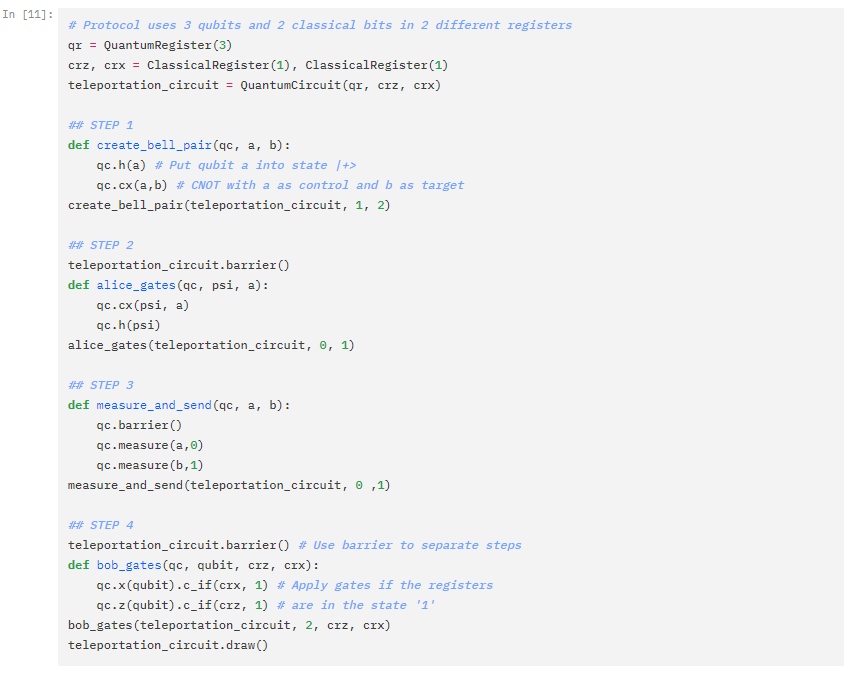
\includegraphics[width=15cm]{9_10.png}
	\label{fig:9-10}
\end{figure}
شکل مدار به صورت \ref{fig:9-11} است. 

\begin{figure}[h]
	\caption{ مدار فرابرد کوانتومی}
	\centering
	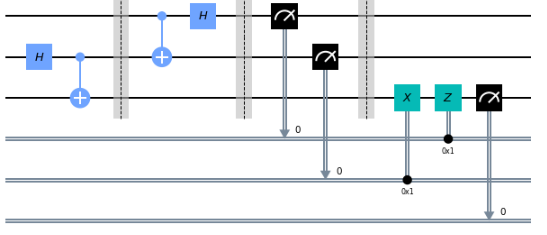
\includegraphics[width=10cm]{9_11.png}
	\label{fig:9-11}
\end{figure}
در نهایت با اندازه‌گیری حالت باب در یک ثبات دیگر می‌توانیم ببینم چگونه آخرین کیوبیت اندازه‌گیری شده همواره $0$ است. 
\begin{figure}[h]
	\caption{نتیجه اجرای کد به تعداد زیاد}
	\centering
	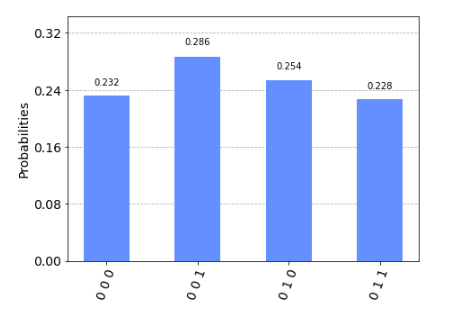
\includegraphics[width=10cm]{9_12.png}
	\label{fig:9-12}
\end{figure}

\section{الگوریتم دوچ-جوزا}
برای یادآوری، مراحل زیر یک اجرای الگوریتم دوچ-جوزا برای تشخیص ثابت یا مجموع صفر بودن تابع $f$ است. 
\begin{enumerate}
	\item دو ثبات کوانتومی آماده می‌کنیم. یکی با $n$ بیت و دیگری با $1$ بیت. اولی را با $0$ مقداردهی اولیه می‌کنیم و دومی را با $1$. 
	\begin{equation}
		\ket{\psi_{0}} = \ket{0}^{\otimes 0}\ket{1}
	\end{equation}
	\item سپس عملگرد هادامارد را روی هر کیوبیت اجرا می‌کنیم. 
	\begin{equation}
		\ket{\psi_{1}} = \frac{1}{\sqrt{2^{n+1}}} \sum_{x=0}^{2^{n}-1} \ket{x}(\ket{0}-\ket{1})
	\end{equation}
	\item جعبه‌ سیاه تابع $f$ را به این صورت اعمال می‌کنیم که در شکل\ref{fig:9-18} نشان داده شده است.
	\begin{equation}
		\begin{split}
		\ket{\psi_{2}} & = \frac{1}{\sqrt{2^{n+1}}} \sum_{x=0}^{2^{n}-1} \ket{x}(\ket{f(x)}-\ket{f(x) \oplus 1}) \\
		& = \frac{1}{\sqrt{2^{n+1}}} \sum_{x=0}^{2^{n}-1} (-1)^{f(x)}\ket{x}(\ket{0}-\ket{1})
		\end{split}
	\end{equation}
	\item در این مرحله، کیوبیت دوم را حذف می‌کنیم و یک بار دیگر هادامارد را اعمال می‌کنیم.  
\begin{equation}
		\begin{split}
		\ket{\psi_{3}} & = \frac{1}{2^{n}} \sum_{x=0}^{2^{n}-1} (-1)^{f(x)}   [\sum_{y=0}^{2^{n}-1} (-1)^{x.y}\ket{y} ]\\
		& = \frac{1}{2^{n}} \sum_{y=0}^{2^{n}-1} [\sum_{x=0}^{2^{n}-1} (-1)^{f(x)} (-1)^{x.y} ]\ket{y} \\
		\end{split}
	\end{equation}
	\item در نهایت با اندازه‌گیری کلیه کیوبیت‌ها، نتیجه‌گیری می‌کنیم. 
\end{enumerate}

\begin{figure}[h]
	\caption{چعبه‌سیاه تابع $f$ }
	\centering
	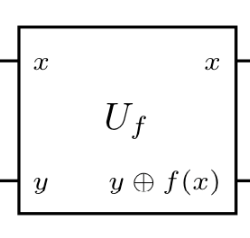
\includegraphics[width=5cm]{9_18.png}
	\label{fig:9-18}
\end{figure} 

در مرحله اول، تلاش می‌کنیم که یک جعبه‌سیاه برای این تابع بسازیم. بدین منظور، لازم است که شکل تابع را مشخص کنیم. فرض کنید عملیات را روی $4$ کیوبیت انجام می‌دهیم. در شکل  \ref{fig:9-13}، دقیقا عملیاتی که در مرحله سوم الگوریتم بالا رخ داد انجام شده است. در این تابع، یک تابع مجموع صفر را برنامه نویسی می‌کنیم.
\begin{figure}[h]
	\caption{کد دوچ-جوزا - جعبه سیاه}
	\centering
	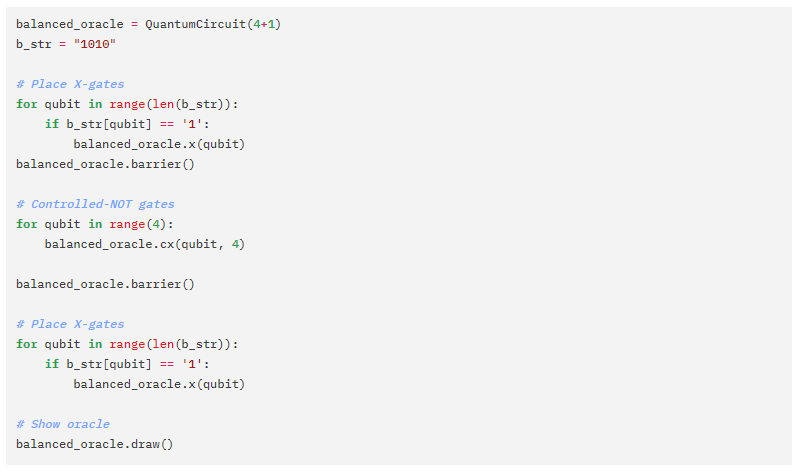
\includegraphics[width=15cm]{9_13.png}
	\label{fig:9-13}
\end{figure}  
که شکل \ref{fig:9-14} این مدار را نشان می‌دهد. 
\begin{figure}[h]
	\caption{مدار دوچ-جوزا - جعبه سیاه}
	\centering
	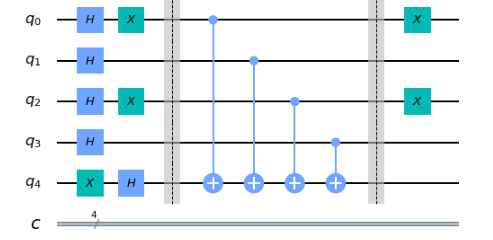
\includegraphics[width=10cm]{9_14.png}
	\label{fig:9-14}
\end{figure}
در ادامه، لازم است ورودی‌ها را بچینیم و مرحله $1$ و $2$ را انجام دهیم. سپس جعبه سیاه را وصله کنیم و مرحله $4$ و $5$ را اعمال کنیم. برای اینکار به شکل \ref{fig:9-15} توجه کنید. 
 
\begin{figure}[h]
	\caption{کد دوچ-جوزا }
	\centering
	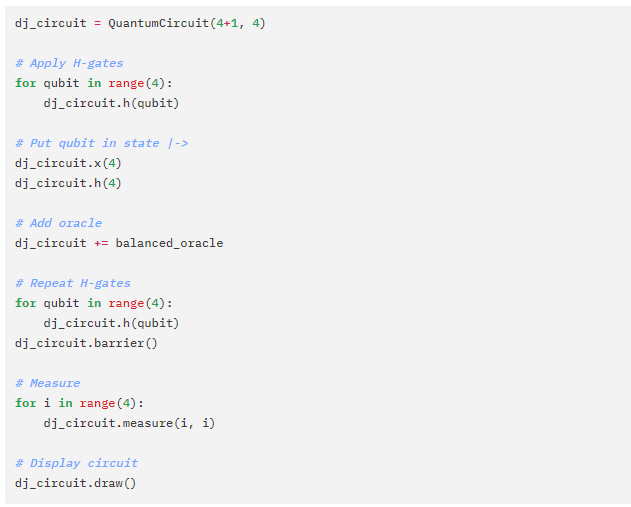
\includegraphics[width=12cm]{9_15.png}
	\label{fig:9-15}
\end{figure}
که مدار آن را در شکل \ref{fig:9-16} می‌بینیم. 
\begin{figure}[h]
	\caption{مدار دوچ-جوزا }
	\centering
	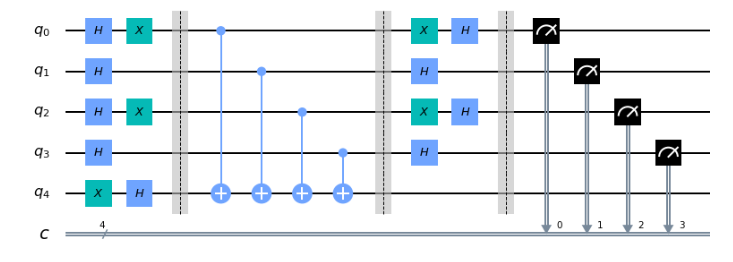
\includegraphics[width=12cm]{9_16.png}
	\label{fig:9-16}
\end{figure}
در نهایت، اجرای چندباره این الگوریتم با این تابع نشان ‌می‌دهد احتمال گرفتن $0000$ در خروجی $0$ است. (شکل \ref{fig:9-17})
\begin{figure}[h]
	\centering
	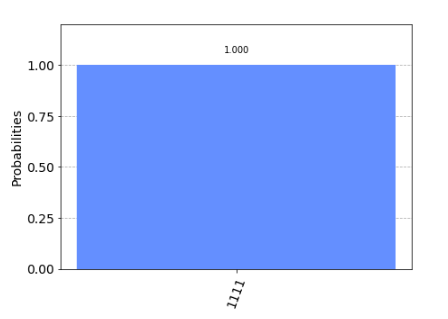
\includegraphics[width=6cm]{9_17.png}
	\caption{نتیجه اجرای چند باره الگوریتم دوچ جوزا. احتمال خروجی 1111 برابر با 100\% به‌دست آمده است.}
	\label{fig:9-17}
\end{figure}
\pagebreak
\section{الگوریتم دوچ-جوزا توزیع‌شده}

در ادامه قسمت قبل، الگوریتم ارائه شده در \autoref{djd} را پیاده‌سازی می‌کنیم.

کد مربوط به این قسمت نسبت به کدهای قبلی‌ طویل‌تر است و ارائه قسمت به قسمت آن در این مجال ممکن نیست. در پیوست دوم (\autoref{ap2})، کل کد تکه به تکه به همراه مدار مربوط به هر قسمت به تفضیل بررسی خواهد شد.\\
 مدار نهایی و نتیجه اجرای کد، در شکل‌های \ref{fig:sim1} و \ref{fig:sim2} آورده‌شده است.
  \begin{figure}
  \centering
 
 \includegraphics[width=.8\linewidth]{output_11_0.png}
 \caption{نتیجه اجرای چندباره الگوریتم دوچ جوزا توزیع شده و ارتباط بین آلیس و باب با ورودی‌های متفاوت.}
 \label{fig:sim2}
 \end{figure}
 \begin{figure}
 \centering
 
 \includegraphics[width=.9\linewidth]{output_8_0.png}
 \caption{مدار نهایی استفاده شده توسط آلیس (بالا) و باب (پایین) در الگوریتم‌ دوچ جوزا توزیع‌شده.}
 \label{fig:sim1}
 \end{figure}
 



% Appendices
\appendix
\section{پیوست: مبانی ریاضی مکانیک کوانتومی}\label{chapter7}
دراین بخش با ریاضیات مورد نیاز برای فهم چارچوب نظری مکانیک کوانتومی آشنا می‌شویم.  مطالب این بخش از  \cite{ 
 		wolf19,
 		qis,
 		nielsen10,
 		strang11
 		}
اقتباس شده است.

  \subsection{فضای برداری}
  مجموعه $V$ را یک فضای برداری روی میدان $F$ می‌گوییم هرگاه دو عمل زیر تعریف شده 
  \begin{equation}
  	+ : V \times V \rightarrow V \quad , \quad . : F \times V \rightarrow V
  \end{equation}
  و دارای خواص زیر باشند: 
   \begin{equation}
   \begin{split}
   A_{1}: & \quad x + y = y + x\\
   A_{2}: & \quad (x + y) + z = x + (y + z)\\
   A_{3}: & \quad \exists 0 \in V | 0 + x = x\\
   A_{4}: & \quad \forall x \in V | -x + x = 0\\
   M_{1}: & \quad \alpha(x+y) = \alpha x + \alpha y\\
   M_{2}: & \quad (\alpha + \beta)x = \alpha x + \beta x\\
   M_{3}: & \quad \alpha(\beta x) = (\alpha\beta) x\\
   M_{4}: & \quad 1x = x
   \end{split}
   \end{equation}
   بسته به این که $F$ میدان اعداد حقیقی یا میدان اعداد مختلط باشد، فضای برداری $V$ را فضای برداری مختلط یا حقیقی گوییم. ازاین به بعد منحصراً با فضاهای برداری مختلط کار می‌کنیم. 
   
\begin{example}
مجموعه‌های زیر هرکدام یک فضای برداری هستند. 
\begin{enumerate}
	\item $R^{n}$ یا مجموعه $n$-تایی‌های مرتب حقیقی
	\item $C^{n}$ یا مجموعه $n$-تایی‌های مرتب مختلط
	\item $M_{m \times n}(F)$ یا مجموعه ماتریس‌های $m \times n$ که درایه‌های آن عناصر یک میدان $F$ هستند.
	\item $P_{n}([a,b])$ یا مجموعه چندجمله‌ای‌های حقیقی مرتبه $n$ از متغیر $x$ که در فاصله $[a,b]$ تعریف شده‌اند. 
	\item $C^{k}[a,b]$ یا مجموعه توابع حقیقی یا مختلط $k$ بار مشتق‌پذیر در بازه $[a,b]$.
\end{enumerate}  
\end{example} 
   
\begin{definition}
   هرگاه $V$ یک فضای برداری و $W \subset V$ یک زیر مجموعه از آن باشد، آنگاه $W$ را یک زیرفضای $V$ گوییم اگر $W$ نسبت به جمع بردارها و ضرب اعداد در بردارها بسته باشد. 
   \end{definition}
   
   \subsection{ضرب داخلی و اندازه}
    \textbf{تعریف:}
    در یک فضای برداری $V$ یک عمل دوتایی $\langle,\rangle : V \times V \rightarrow C$ را یک ضرب داخلی می‌نامیم هرگاه در شرایط زیر صدق کند:
    \begin{equation}
    	\langle x , y + \alpha z \rangle = \langle x , y \rangle + \alpha \langle x , z \rangle
    \end{equation}
    
    \begin{equation}
    	\langle x , y \rangle = \langle y , x \rangle^{*}
    \end{equation}
    \begin{equation}
    	\langle x , x \rangle \geq 0
    \end{equation}
    \begin{equation}
    	\langle x , x \rangle =  0 \rightarrow x = 0
    \end{equation}
    فضایی را که به ضرب داخلی مجهز شده باشد یک فضای برداری ضرب داخلی می‌گوییم. 
    \begin{theorem}
    کوشی-شوارتز:
     در فضای ضرب داخلی داریم:
\begin{equation}
 	|\langle x,y \rangle | = \langle x,x \rangle \langle y,y \rangle .
 \end{equation}
    \end{theorem}

\begin{definition}{اندازه یک بردار: }
در هر فضای ضرب داخلی، می‌توان اندازه یک بردار را به شکل زیر تعریف کرد:
\begin{equation}
	|x| := \sqrt{\langle x,x \rangle}
\end{equation}
\end{definition}
با توجه به نامساوی کوشی-شوارتز می‌توان نوشت:
\begin{equation}
	 	|\langle x,y \rangle | = |x||y|
\end{equation}


\begin{definition}{فضای نرم یا اندازه‌دار: }
یک فضای برداری $V$ که در آن نگاشت $\| \quad \| : V \rightarrow R$ تعریف شده باشد را فضای برداری اندازه‌دار\footnote{Normed Vector Space} می‌گوییم هرگاه شرایط زیر برقرار باشد:
\begin{equation}
	\| v \| \geq 0 \quad \forall v
\end{equation}
\begin{equation}
	\| v \| = 0 \rightarrow v = 0
\end{equation}
\begin{equation}
	\| \alpha v \| = |a| \|v \|
\end{equation}
\begin{equation}
\| v + w \| \leq \| v \| + \| w \|
\end{equation}
\end{definition}
هرفضای ضرب داخلی باهمان اندازه‌ای که از روی ضرب داخلی تعریف می‌شود یک فضای اندازه‌دار است، ولی یک فضای اندازه‌دار الزاماً یک فضای ضرب داخلی نیست. به عبارت دیگر، اندازه لزوما از روی ضرب داخلی تعریف نشده است. برای مثال، برای فضای توابع $C[a,b]$ نگاشت $\| f \| = sup_{x \in [a,b]} | f(x)|$ یک اندازه است که از روی ضرایب داخلی تعریف نشده‌ است. 

\subsection{پایه}
پایه به‌هنجار\footnote{Normal} $\{ e_{i}, i = 1,...,N\}$ را برای فضای برداری $V$ در نظر می‌گیریم. به‌هنجار بودن به معنای آن است که $\langle e_{i},e_{j} \rangle = \delta_{ij}$. هر بردار $x \in V$  را می‌توان بر حسب این بردار‌های پایه بسط داد و نوشت:
\begin{equation}
	x = \sum_{i = 1} ^{N} x_{i}e_{i}
\end{equation}
بدیهی است که 
\begin{equation}
	x_{i} = \langle e_{i},x \rangle
\end{equation}


پایه‌ها را می‌توان با یک ماتریس تبدیل پایه دو بعدی مانند $S$ به یک دیگر تبدیل کرد. برای مثال، فرض کنید که بردار $x$ را که در پایه $e_{i}$ است را می‌خواهیم در پایه $e^{'}_{i}$ بنویسیم. لازم است درایه‌های ماتریسی آن را استخراج کنیم. در نظر بگیرید $e^{'}_{i} = S_{li}e_{l}$:
\begin{equation}
x^{'}_{i} = \langle e^{'}_{i},x \rangle = \langle S_{li}e_{l}, x \rangle = S_{li}x_{l}
\end{equation}
و یا به صورت فشرده‌تر:
\begin{equation}
	x^{'} = xS.
\end{equation}
از آنجا که پایه‌های $\{e_{i}\}$ و $\{e^{'}_{i}\}$ هر دو بهنجار هستند به راحتی نتیجه می‌گیریم که ماتریس تبدیل پایه $S$ در شرط زیر صدق می‌کند:
\begin{equation}
S^{\dagger}S = I
\end{equation}
چنین ماتریسی را ماتریس‌های یکانی\footnote{Unitary} می‌گوییم.

که در آن $S^{\dagger}$ ماتریس الحاقی\footnote{Conjugate Transpose} $S$ است و چنین تعریف می‌شود:

\begin{equation}
S^{\dagger} = (S^{*})^{T} \quad or \quad S^{\dagger}_{ij} = (S^{*})_{ji}
\end{equation}
همچنین هرگاه ماتریس با الحاقی خود برابر باشد، آن را ماتریس هرمیتی می‌گوییم: 
\begin{equation}
	S^{\dagger} = S.
\end{equation}
%TODO example??

\subsection{فضای کامل و هیلبرت}
\begin{definition}{دنباله کوشی:}
در یک فضای برداری، دنباله‌ای از بردارها مانند $\{x_{1},x_{2},...,x_{n},...\}$  درنظر می‌گیریم. این دنباله، یک دنباله کوشی نامیده می‌شود هر گاه فاصله بین  بردارها به تدریج کم شود؛ به عبارت دقیق‌تر، هرگاه به ازای هر $\epsilon > 0$ عددی مانند $N$ یافت شود که 
\begin{equation}
	\forall m,n > N \rightarrow |x_{n} - x_{m} | \leq \epsilon
\end{equation} 
\end{definition}
در یک فضای برداری، لزوما حد کوشی در خود فضا قرار ندارد. مثلا، هرگاه میدان اعداد گویا را به عنوان یک فضای برداری روی خودش درنظر بگیریم، دنباله $\{ ( 1 + \frac{1}{n})^{n} \}$ اگرچه یک دنباله کوشی است، ولی حد آن در میان اعداد گویا قرار ندارد. با افزودن اعداد گنگ به میدان، یک فضای برداری میدان حقیقی به دست می‌آید که کامل است. 

\begin{definition}
یک فضای برداری را فضای برداری کامل گوییم هرگاه حد دنباله کوشی را در خود داشته باشد. 
\end{definition}
 
\begin{definition}
 یک فضای برداری با ضرب داخلی کامل را فضای هیلبرت\footnote{Hilbert Space}  می‌نامیم. از آنجایی که میدان اعداد حقیقی و مختلط کامل است، می‌توان ثابت کرد هر فضا با بعد محدود روی این میدان‌ها هیلبرت است. 
 \end{definition}
 
\subsection{تبدیلات خطی}
در یک فضای برداری  $V$، نگاشت 
$\hat{T} : V \rightarrow V$ را یک تبدیل خطی یا یک عملگر خطی\footnote{Linear Operator} می‌گوییم هرگاه داری خاصیت زیر باشد:
\begin{equation}
	\hat{T}(x + \alpha y ) = \hat{T}(x) + \alpha \hat{T}(y) \quad \forall \alpha \in F, x,y \in V
\end{equation}
ماتریس $T$ با درایه‌های $T_{mn}$ را ماتریس مربوط به تبدیل خطی $\hat{T}$ در پایه $\{e_{i}\}$ می‌گوییم. هرگاه پایه فوق به‌هنجار باشد، می‌توانیم بنویسیم 
\begin{equation}
	\langle e_{j}, \hat{T}e_{i} \rangle = T_{ji}
\end{equation}
تاثیر تابع $\hat{T}$ روی بردار $x$ عبارت است از:
\begin{equation}
	\hat{T}x = \hat{T}x_{i}e_{i} = x_{i}(\hat{T}e_{i}) = x_{i}T_{ji}e_{j} = (T_{ji}x_{i})e_{j} = (Tx)_{j}e_{j}
\end{equation}
که برابر با ضرب از سمت چپ ماتریس $T$ روی $x$ است. 

همچنین، با تعویض پایه، ماتریس تغییر می‌یابد:
\begin{equation}
	T^{'}_{ij} = \langle e^{'}_{i},\hat{T}e^{'}_{j} \rangle = \langle S_{li}e_{l},\hat{T}S_{mj}e_{m} \rangle = S^{*}_{li}T_{lm}S_{mj}
\end{equation}
که به صورت زیر قابل بازنویسی است:
\begin{equation}
T^{'} = S^{\dagger}TS
\end{equation}

هرگاه $A$ و $B$ دو تبدیل خطی دلخواه روی $V$ و $\alpha$ عددی دلخواه متعلق به میدان $F$ باشد، آنگاه $\alpha A+B$ نیز یک تبدیل خطی روی $V$ است. درنتیجه، مجموعه تبدیلات خطی روی $V$ تشکیل یک فضای برداری می‌دهند که آن را با $End(V)$ نشان می‌دهیم. همچنین، ضرب دو تبدیل خطی با تعریف 
\begin{equation}
	(AB)x := A(Bx)
\end{equation}
 نیز یک تبدیل خطی است. پس می‌توان گفت که $End(V)$ نه تنها یک فضای برداری است بلکه یک جبر است که خاصیت شرکت پذیری دارد ($(AB)C = A(BC)S$) ولی جبر جابه‌جایی ندارد ($AB \ne BA$) اما یکه‌دار\footnote{Unital} است که یعنی عنصری دارد مانند $I$ که $AI = IA = A$. 
 
 دیدیم که به یک عملگر خطی می‌توان یک ماتریس نسبت داد. وقتی که پایه فضا را معین می‌کنیم، بین فضای تبدیلات خطی یعنی $End(V)$ و فضای ماتریس‌های $M_{n \times n}(C)$ یک نگاشت یک به یک خواهیم داشت. بنابراین یک تبدیل خطی و ماتریس آن به جای هم قابل استفاده هستند. همچنین، با تبدیل زیر می‌توان فضای تبدیل خطی روی $V$ را به یک فضای ضرب داخلی تبدیل کرد:
  \begin{equation}
  	\langle A,B \rangle = tr(AB^{\dagger})
  \end{equation}
  که در آن رد\footnote{Trace} ماتریس $tr(A)$ برای ماتریس مربعی $A$ برابر با مجموعه درایه‌های قطر اصلی است.
  
  \subsection{جمع نیمه‌مستقیم دو زیرفضا}
  
\begin{definition}
  هرگاه $V$ یک فضای برداری و $U$ و $W$ دو زیرفضای آن باشند، $U + W$ را به عنوان مجموعه زیر تعریف می‌کنیم:
  \begin{equation}
  	U + W := \{ v | v = u + w, u \in U, w \in W \}
  \end{equation}
   واضح است که $U + W$ نیز یک زیرفضا برای $V$ است. 
   \end{definition}
 \begin{definition}
   فرض کنید که $V$ یک فضای برداری و $W$ و $U$ دو زیرفضای آن باشند به طوری که:
   \begin{enumerate}
   \item $V = W + U$
   \item تنها بردار مشترک $U$ و $W$ بردار صفر باشد. 
   \end{enumerate}
   در این صورت $V$ جمع نیمه‌مستقیم\footnote{Semi-direct Sum} $U$ و $W$ می‌گوییم و می‌نویسیم 
   \begin{equation}
   V = U \oplus W
   \end{equation}
   \end{definition}
   \begin{theorem}
   $V = W \oplus U$ اگر و تنها اگر هر بردار $v \in V$ را بتوان به صورت $u + w$ یکتایی نوشت که در آن $u \in U$  و  $w \in W$. 
   \end{theorem}
   \begin{theorem}
   اگر $V = U + W$ آنگاه $dim(V) = dim(U) + dim(W)$. 
   \end{theorem}
   \begin{definition}
   فرض کنید که $V = V_{1} \oplus V_{2} \oplus ... \oplus V_{r}$. در این صورت، هر بردار $v \in V$ به صورت یکتای $v = v_{1} + v_{2} + ... + v_{r}$ تجزیه می‌شود. $P_{j}$ را عملگری تعریف کنید که:
   \begin{equation}
   		P_{j}v = v_{j}
   \end{equation}
   در این صورت، $P_{j}$ را عملگر تصویر روی زیرفضای  $V_{j}$ می‌خوانیم. 
   \end{definition}
   \begin{theorem}
   عملگرهای تصویری\footnote{Image Operators} خواص زیر را دارند:
   \begin{enumerate}
   	\item $P_{j}P_{k} = \delta_{jk}P_{j}$
   	\item $\sum_{j=1}^{r} P_{j} = I$
   \end{enumerate}
   \end{theorem}
   \begin{theorem}
   هرگاه $V$ یک فضای ضرب داخلی باشد و $V = \bigoplus_{j=1}^{r} V_{j}$ که در آن $V_{j}$ها بر هم عمود هستند، آنگاه عملگرهای $P_{j}$ هرمیتی\footnote{Hermitian} هستند. 
   \end{theorem}
   \subsection{مساله ویژه‌مقدار}
   عملگر $T: V \rightarrow V$ را درنظر می‌گیریم. مساله ویژه‌مقدار\footnote{Eigenvalue} عبارت است از یافتن بردارهای غیرصفری که تحت اثر $T$ به مضربی از خود تبدیل بشوند: 
   \begin{equation}
   Tx = \lambda x
   \end{equation}
    بردار $x$ غیرصفر خواهد بود هرگاه ماتریس $T - \lambda I$ وارون‌پذیر نباشد، یعنی این‌که
    \begin{equation}
    	det(T-\lambda I) = 0
    \end{equation}
    این معادله، یک معادله درجه $N$ است که در حوزه اعداد مختلط حتما $N$ جواب مانند  $\{ \lambda_{i}, i = 1,...,N\} $ دارد که به آن‌ها ویژه‌مقدارهای تبدیل $T$ گوییم. این جواب‌ها لزوما با هم متفاوت نیستند. 
    
    بردار مربوط به $\lambda_{i}$ که در معادله $Tv_{i} = \lambda_{i} v_{i}$ صدق می‌کند را ویژه‌بردار\footnote{Eigenvector} متناظر با آن ویژه‌مقدار می‌خوانیم. هرگاه $x$ و $y$ ویژه‌بردارهای مربوط به $\lambda$ باشند، بدیهی است که هر ترکیب خطی از آن‌ها هم ویژه‌برداری از $\lambda$ است. بنابراین، مجموعه بردارهای متعلق به یک ویژه‌مقدار تشکیل یک زیرفضا را می‌دهند که به آن ویژه‌فضای\footnote{Eigenspace} آن ویژه‌مقدار می‌گویند. 
    
    \subsection{عملگرهای هرمیتی، یکانی و به‌هنجار}
    
    \begin{definition}
    در یک فضای ضرب داخلی، الحاقی یک عملگر $T$ عملگری مانند $T^{\dagger}$ است که در شرط زیر صدق کند: 
    \begin{equation}
    	\langle v,Tw \rangle = \langle T^{\dagger}v,w \rangle
    \end{equation}
    \end{definition}
    با استفاده از این تعریف می‌توان به راحتی خواص زیر را ثابت کرد:
    \begin{enumerate}
    	\item الحاقی یک عملگر خطی خود نیز یک عملگر خطی است.
    	\item $(cA + B)^{\dagger} = c^{*}A^{\dagger} + B^{\dagger}$
    	\item $AB)^{\dagger} = B^{\dagger}A^{\dagger}$
    	\item $(A^{\dagger})^{\dagger} = A$
    \end{enumerate}
     
      \begin{definition}
     در یک فضای ضرب داخلی عملگر هرمیتی به عملگری گفته می‌شود که در شرط $T^{\dagger} = T$ صدق کند. عملگر پادهرمیتی به عملگری گفته می‌شود که در شرط $T^{\dagger} = -T$ صدق کند. 
     \end{definition}
     \begin{definition}
     در یک فضای ضرب داخلی، عملگر یکانی $U$ به عملگری گفته می‌شود که ضرب داخلی بردارها رو حفظ کند، یعنی 
      \begin{equation}
      	\langle Uv,Uw \rangle = \langle v,w \rangle
      \end{equation}
      چنین عملگری در شرط $UU^{\dagger} = U^{\dagger}U$ صدق می‌کند. 
      \end{definition}
      \begin{definition}
      عملگر نرمال یا به‌هنجار عملگری است که با الحاقی خود جابه‌حا شود. عملگرهای هرمیتی و یکانی نرمال هستند. 
      \begin{equation}
      	AA^{\dagger} = A^{\dagger}A
      \end{equation}
      \end{definition}
      \begin{theorem}
      فرض کنید که $A$ یک عملگر به‌هنجار است. در این صورت اگر $Ax = \lambda x$ آنگاه $A^{\dagger} x = \lambda^{*} x$.
      \end{theorem}
      \textbf{نتیجه: }
      ویژه‌مقادیر یک عملگر هرمیتی حقیقی هستند. 
      
      \begin{theorem}
      ویژه‌بردارهای متناظر با ویژه‌مقدارهای متمایز یک عملگر به‌هنجار بر هم عمودند. 
      \end{theorem}
      \begin{definition}
      عملگر مثبت نیمه معین\footnote{Positive Semidefinite} عملگری است که
       \begin{equation}
       	\forall v \in V: \quad \langle x,Tx \rangle \geq 0
       \end{equation}
       همچنین عملگر مثبت معین\footnote{Definite Positive} عملگری است که
        \begin{equation}
       	\forall v \in V: \quad \langle x,Tx \rangle > 0
       \end{equation} 
       \end{definition}

  اگر $f: \mathbb{R} \rightarrow \mathbb{R}$ یک تابع و $A: \mathcal{H} \to \mathcal{H}$ عملگری هرمیتی و به صورت زیر باشد:
    \begin{equation}
    	A = \sum_{i=0}^{d-1} \lambda_{i} \dyad{v_{i}}{v_{i}}
    \end{equation}
    آنگاه تعریف می‌کنیم: 
    \begin{equation}
    	f(A) := \sum_{i=0}^{d-1} f(\lambda_{i}) \dyad{v_{i}}{v_{i}}
    \end{equation}
    
    توجه کنید که ویژه‌مقادیر $f(A)$ برابر با $f(\lambda_{i})$ها هستند که $\lambda_{i}$ها ویژه‌مقادیر $A$ هستند. 
    
      \subsection{نمادگذاری دیراک}
      یک فضای برداری $V$ با بعد $N$ با پایه‌های به‌هنجار $\{e_{1}, e_{2}, e_{3}, ... , e_{N}\}$ درنظر می‌گیریم. هر بردار $v \in V$ بسطی از بردارهای پایه به شکل زیر است: 
      \begin{equation}
      	v = \sum_{i=1}^{N} v_{i}e_{i}
      \end{equation}
      ضرب داخلی این بردار در خودش به صورت زیر نوشته می‌شود:
      \begin{equation}
      	\langle v,v \rangle = \sum_{i=1}^{N} v^{*}_{i} v_{i}
      \end{equation}
       می‌توان به ازای چنین برداری، یک بردار ستونی با نماد $\ket{v}$ و یک بردار سطری با نماد $\bra{v}$ به شکل زیر تعریف کرد:
       \begin{equation}
       	\ket{v} = \begin{pmatrix}
       		v_{1} \\ \\ v_{2} \\ \\ \vdots \\ \\ v_{N} 
       	\end{pmatrix}
       \end{equation}
       \begin{equation}
       	\bra{v} = \begin{pmatrix}
       		v^{*}_{1} & v^{*}_{2} & \cdots & v^{*}_{N} 
       	\end{pmatrix}
       \end{equation}
       
       بردار $\bra{v}$ را یک بردار $bra$ و بردار $\ket{v}$ یک بردار $ket$ می‌نامیم. توجه کنیم که ‌می‌توانیم این دو بردار را در هم ضرب کنیم:
       \begin{equation}
       		\bra{v}\ket{v} = \sum_{i=1}^{N} v^{*}_{i}v_{i} = \langle v,v \rangle
       \end{equation}
       بردار‌های پایه $e_{1}, ... , e_{N}$ نیز شکل زیر را پیدا می‌کنند:
       

\begin{multicols}{3}

$\ket{1} = \begin{pmatrix} 1 \\ \\ 0 \\ \\ \vdots \\ \\ 0 \end{pmatrix}$
  \columnbreak{}
$\ket{2} = \begin{pmatrix} 0 \\ \\ 1 \\ \\ \vdots \\ \\ 0 \end{pmatrix}$
  \columnbreak{}
$\ket{N} = \begin{pmatrix} 0 \\ \\ 0 \\ \\ \vdots \\ \\ 1 \end{pmatrix}$

\end{multicols}
\begin{flushleft}
$\bra{1} = \begin{pmatrix} 1 & 0 & \cdots & 0 \end{pmatrix}$
\\
$\bra{2} = \begin{pmatrix} 0 & 1 & \cdots & 0 \end{pmatrix}$
\\
$\bra{N} = \begin{pmatrix} 0 & 0 & \cdots & 1 \end{pmatrix}$
\\
\end{flushleft}

بنابراین داریم 
\begin{equation}
	\ket{v} = \sum_{i=1}^{N} v_{i}\ket{i}
\end{equation}

\begin{equation}
	\bra{v} = \sum_{i=1}^{N} v^{*}_{i}\bra{i}
\end{equation}

از این به بعد تمامی بردارها را با این نماد‌گذاری نشان می‌دهیم. 

خواص زیر برای این نمادگذاری وجود دارد:
 \begin{enumerate}
 	\item $\bra{v}\ket{w} = \langle v,w \rangle$
 	\item $\bra{v}\ket{w+w^{'}} = \bra{v}\ket{w} + \bra{v}\ket{w^{'}}$
 	\item $\bra{v}\ket{cw} = c\bra{v}\ket{w}$
 	\item $\bra{cv}\ket{w} = c^{*}\bra{v}\ket{w}$
 	\item $\bra{v}\ket{v} \geq 0$
 	\item $\bra{v}\ket{v} = 0 \rightarrow \ket{v} = \bra{v} = 0$
 	\item $\ket{v} = \sum_{i=1}^{N} v_{i}\ket{i}$
 	\item $\bra{i}\ket{v} = v_{i}$
 	\item $\ket{v}\bra{w} := \begin{pmatrix}
 		v_{1}w^{*}_{1} & v_{1}w^{*}_{2} & v_{1}w^{*}_{3} & \cdots & v_{1}w^{*}_{n} \\ 
 		\\
 		v_{2}w^{*}_{1} & v_{2}w^{*}_{2} & v_{2}w^{*}_{3} & \cdots & v_{2}w^{*}_{n} \\ 
 		\\
 		v_{3}w^{*}_{1} & v_{3}w^{*}_{2} & v_{3}w^{*}_{3} & \cdots & v_{3}w^{*}_{n} \\ 
 		\\
 		\vdots & \vdots & \vdots & \ddots & \vdots
		\\
 		v_{N}w^{*}_{1} & v_{N}w^{*}_{2} & v_{N}w^{*}_{3} & \cdots & v_{N}w^{*}_{n} \\ 

 	\end{pmatrix}$
 	\item $\ket{v}\bra{w+w^{'}} = \ket{v}\bra{w} + \ket{v}\bra{w^{'}}$
 	\item $\ket{v}\bra{cw} = c^{*}\ket{v}\bra{w}$
 	\item $\ket{cv}\bra{w} = c\ket{v}\bra{w}$
 	\item $\bra{i}\ket{j} = \delta_{ij}$
 	\item $\sum_{i} \ket{i}\bra{i} = I$
 	\item $\ket{v} = I\ket{v} = \sum_{i=1}^{N}  \ket{i}\bra{i}\ket{v} = \sum_{i=1}^{N} v_{i}\ket{i}$
 	\item $T = \sum_{j} \ket{j}\bra{i}T\sum_{i} \ket{i}\bra{i}  = \sum_{i,j}T_{ji}\ket{j}\bra{i}$
 	\item $\mel{i}{AB}{j} = \sum_{k} \mel{i}{AB}{k} \mel{k}{AB}{j} $
 \end{enumerate}
 \subsection{ضرب تنسوری}
 هرگاه $(A)_{m \times n}$ و $(B)_{p \times q}$ دو ماتریس با ابعاد داده شده باشند، می‌توان ضرب تنسوری‌\footnote{Tensor Product} آن‌ها را که ماتریسی با ابعاد $mp \times nq$ است را به شکل زیر تعریف کرد
 
 \begin{equation}
 	(A \otimes B)_{ij,kl} := A_{ik}B_{jl}
 \end{equation}
 به لحاظ عملی ضرب این دو ماتریس به شکل زیر محاسبه می‌شود:
 
\begin{equation}
 A \otimes B := \begin{pmatrix}
 		a_{11}B & a_{12}B & a_{13}B & \cdots & a_{1n}B \\ 
 		\\
 		a_{21}B & a_{22}B & a_{23}B & \cdots & a_{2n}B \\ 
 		\\
 		a_{31}B & a_{32}B & a_{33}B & \cdots & a_{3n}B \\ 
 		\\
 		\vdots & \vdots & \vdots & \ddots & \vdots
		\\
 		a_{m1}B & a_{m2}B & a_{m3}B & \cdots & a_{mn}B \\ 

 	\end{pmatrix}
 \end{equation} 

 	
 	ضرب تنسوری خواص زیر را دارد:
 	
 	\begin{enumerate}
 		\item $A \otimes (B + C) = A \otimes B + A \otimes C$
 		\item $A \otimes (\alpha B) = (\alpha A) \otimes B = \alpha (A \otimes B)$
 		\item $(A \otimes B) \otimes C = A \otimes ( B \otimes C)$
 		\item $(A \otimes B)(C \otimes D) = AC \otimes BD$
 		\item $(A \otimes B)^{\dagger} = A^{\dagger} \otimes B^{\dagger}$
 	\end{enumerate}
 	حال اگر فضای برداری $V$  با بردارهای پایه  $\{\ket{i}, i = 1, ..., m\}$ و فضای برداری $W$ با بردارهای پایه $\{\ket{\mu}, \mu = 1, ..., m\}$ را درنظر بگیریم، می‌توان ضرب تنسوری بردارهای پایه را مطابق با تعریف بالا به دست آوریم. به ترتیب بردار پایه به شکل $\ket{i} \otimes \ket{\mu}$ به دست می‌آوریم که آن‌ها را به اختصار با $\ket{i,\mu}$ نشان می‌دهیم. این بردارهای جدید یک فضای برداری جدید را جاروب\footnote{Span} می‌کنند که با بعد $mn$ است که آن را فضای برداری ضرب تنسوری $W$ و $V$ می‌خوانیم. 
 	

نکته آخر این است که یک بردار دلخواه در فضای $V \otimes W$ را نمی‌توان به صورت ضرب‌های $\ket{v} \otimes \ket{w}$ نوشت؛ مثل بردار زیر
\begin{equation}
	\ket{\psi} := \ket{0,0} + \ket{1,1}
\end{equation}
	این نکته ما را دعوت می‌کند که در مورد خاصیت در‌هم‌تنیدگی در مکانیک کوانتومی بیشتر بررسی کنیم. 


% References
\renewcommand{\bibname}{References}
\addcontentsline{toc}{section}{مراجع}

\begin{latin}
\bibliography{ref}
\end{latin}

%\include{abstract_english}
%%***************************
% last page: Blank
%***************************
\thispagestyle{empty}
\mbox{}

% It's finally over. Wasn't that hard, was it?

\end{document}
